%%%%%%%%%%%%%%%%%%%%%%%%%%%%%%%%%%%%%%%%%%%%%%%%%%%%%%%%%%%%%%%%%%%%%%
% Lớp 12 | Nguyên hàm, tích phân | Ứng dụng thực tế và hình học của tích phân
% Dạng 2D4?3-1: Diện tích hình phẳng được giới hạn bởi các đồ thị
% Số câu: 131  (sinh tự động bởi tach_cau.py; từ nay thầy sửa trực tiếp file này)
%%%%%%%%%%%%%%%%%%%%%%%%%%%%%%%%%%%%%%%%%%%%%%%%%%%%%%%%%%%%%%%%%%%%%%

%%%%%%%%%%%%%%%% TRẮC NGHIỆM 4 PHƯƠNG ÁN %%%%%%%%%%%%%%%%

% nguồn: Phan1_Lop_12_Dai_so_Chuong_4
\begin{ex}%[2D4N3-1]%[ma:e50c7987]
	Diện tích hình phẳng giới hạn bởi đồ thị hàm số $y=\sqrt{1+3x}$,  trục $Ox$ và hai đường thẳng $x=0$, $x=1$ bằng
	\choice 
		{\True $\displaystyle\int_0^1  \sqrt{1+3x}\mathrm{\,d}x$}
		 {$\pi \displaystyle\int_0^1 \sqrt{1+3x}\mathrm{\,d}x$}
		 {$\displaystyle\int_0^1 (1+3x)\mathrm{\,d}x$}
		{$\pi\displaystyle\int_0^1  (1+3x)\mathrm{\,d}x$}
	\loigiai{Trên đoạn $[0;1]$, $y=\sqrt{1+3x}>0$. \\ 
		Diện tích hình phẳng giới hạn bởi đồ thị  hàm số $y=\sqrt{1+3x}$, trục $Ox$ và hai đường thẳng $x=0$, $x=1$ là $S=\displaystyle\int_0^1 \sqrt{1+3x}\mathrm{\,d}x$.
	} 
\end{ex}

% nguồn: Phan1_Lop_12_Dai_so_Chuong_4
\begin{ex}%[2D4N3-1]%[ma:cb1fc555]
	Diện tích hình phẳng giới hạn bởi đồ thị hàm số $y=f(x)$, trục $Ox$ và hai đường thẳng $x=a$, $x=b$  $(a < b)$ được tính theo công thức
	 \choice
		{$S=\displaystyle\int_a^b  f(x) \mathrm{\,d}x$}
		{$S=\pi \displaystyle\int_a^b f(x)  \mathrm{\,d}x$}
		{$S=\pi  \displaystyle\int_a^b|f(x)|\mathrm{\,d}x$}
		{\True $S=\displaystyle\int_a^b|f(x)|\mathrm{\,d}x$} 
	\loigiai{Diện tích hình phẳng giới hạn bởi đồ thị hàm số $y=f(x)$, trục $Ox$ và hai đường thẳng $x=a$, $x=b$ $(a < b)$ được tính  theo công thức $S=\displaystyle\int_a^b|f(x)|\mathrm{\,d}x$.}
\end{ex}

% nguồn: Phan1_Lop_12_Dai_so_Chuong_4
\begin{ex}%[2D4N3-1]%[ma:b56b24a0]
	Cho hàm số $y=f(x)$ liên tục trên $[1; 3]$. Diện  tích hình phẳng giới hạn bởi đồ thị hàm số $y=f(x)$, trục hoành và các đường thẳng $x=1$, $x=3$ là
	\choice 
		{\True  $S=\displaystyle\int_1^3|f(x)|\mathrm{\,d}x$}
		{$S=\displaystyle\int_3^1|f(x)|\mathrm{\,d}x$} 
		 {$S=-\displaystyle\int_1^3f(x)\mathrm{\,d}x$}
		{$S=\displaystyle\int_1^3f(x)\mathrm{\,d}x$} 
	\loigiai{ 
		Diện tích hình phẳng cần tính  là $S=\displaystyle\int_1^3|f(x)|\mathrm{\,d}x$.
	} 
\end{ex}

% nguồn: Phan1_Lop_12_Dai_so_Chuong_4
\begin{ex}%[2D4N3-1]%[ma:b13b789d]
	Tính diện tích $S$ của  hình phẳng giới hạn bởi các đường $y=x^2+4$, trục hoành, $x=0$, $x=1$.
	\choice 
		{$\dfrac{13}{3} \pi$} 
		{\True $\dfrac{13}{3}$} 
		{$\dfrac{13}{6}$} 
		 {$\dfrac{13}{6} \pi$}
	\loigiai{ 
		 Ta có $S=\displaystyle\int_0^1\left|x^2+4\right|\mathrm{\,d}x=\displaystyle\int_0^1\left(x^2+4\right) \mathrm{\,d}x=\left.\left(\dfrac{x^3}{3}+4x\right)\right|_1 ^4=\dfrac{13}{3}$.
	 }
\end{ex}

% nguồn: Phan1_Lop_12_Dai_so_Chuong_4
\begin{ex}%[2D4N3-1]%[ma:0e1825d0]
	Cho hàm số $y=f(x)$ xác  định và liên tục trên đoạn $[a;b]$. Diện tích hình phẳng giới hạn bởi đồ thị hàm số $y=f(x)$, trục hoành và hai đường thẳng $x=a$, $x=b$ được tính theo công thức
	 \choice
		{\True $\displaystyle\int_a^b  |f(x)|\mathrm{\,d}x$}
		{$\displaystyle\int_b^a |f(x)|\mathrm{\,d}x$} 
		{$\left|\displaystyle\int_a^b  f(x)\mathrm{\,d}x\right|$}
		{$\displaystyle\int_a^b f(x)\mathrm{\,d}x$} 
	\loigiai{ 
		Diện tích hình phẳng giới hạn bởi đồ thị hàm số $y=f(x)$, trục hoành và hai đường thẳng  $x=a$, $x=b$ được tính theo công thức $\displaystyle\int_a^b |f(x)|\mathrm{\,d}x$.
	 }
\end{ex}

% nguồn: Phan1_Lop_12_Dai_so_Chuong_4
\begin{ex}%[2D4N3-1]%[ma:70dc84d8]
	Tính diện tích $S$ của hình phẳng giới hạn bởi các đường $y=x^2+x$; $y=x$; $ x=4$  và trục tung.
	 \choice
		{$\dfrac{64}{3}  \pi$}
		{\True $\dfrac{64}{3}$} 
		 {$\dfrac{128}{3}$}
		{$\dfrac{128}{3} \pi$} 
	 \loigiai{
	Ta có $S=\displaystyle\int_0^4\left|x^2+x-x\right|\mathrm{\,d}x=\displaystyle\int_0^4x^2\mathrm{\,d}x=\left.\left(\dfrac{x^3}{3}\right)\right|_0  ^4=\dfrac{64}{3}$.}
\end{ex}

% nguồn: Phan1_Lop_12_Dai_so_Chuong_4
\begin{ex}%[2D4N3-1]%[ma:183e34d7]
	\immini{Cho đồ thị hàm số $y=2^{-\frac{x}{2}}$ và hình phẳng được tô màu trong hình bên. Hình phẳng đó được giới hạn bởi các đường nào dưới  đây?
	\choice 
		{\True $y=2^{-\frac{x}{2}}$,  $y=0$, $x=-2$, $x=0$}
		{$y=2^{-\frac{x}{2}}$, $y=0$} 
		{$y=2^{-\frac{x}{2}}$, $x=-2$, $x=0$} 
		{$y=2^{-\frac{x}{2}}$, $y=0$,  $x=-2$, $x=1$}
		 }{
		\begin{tikzpicture}[>=stealth,scale=1,font=\footnotesize]
				\def\xmin{-3}; \def\xmax{1}; \def\ymin{-1}; \def\ymax{3}; 
				\draw[->] (\xmin,0)--(\xmax,0)  node[below right] {$x$};
				\draw[->] (0,\ymin)--(0,\ymax)  node[left] {$y$};
				\begin{scope}
					\clip (\xmin,\ymin) rectangle  (\xmax,\ymax);
					\draw[samples=200,domain=\xmin:\xmax,smooth,variable=\x] plot (\x,{2^(-(\x)/2)}); 
					 \fill[pattern=north west lines]
						 plot[domain=-2:0] (\x,{2^(-(\x)/2)})--(0,1) --
						plot[domain=0:-2] (\x,{0})--(-2,0) --  cycle;
				\end{scope}
				\draw (-2,0)--(-2,2); 
				\draw (-2,0) circle  (1pt) node[below]{$-2$}
					(0,0) circle (1pt) node[below left]{$O$}; 
			\end{tikzpicture}
		} 
	 \loigiai{
		 Hình phẳng trong hình vẽ được giới hạn bởi các đường $y=2^{-\frac{x}{2}}$, $y=0$, $x=-2$, $x=0$.
	 }
\end{ex}

% nguồn: Phan1_Lop_12_Dai_so_Chuong_4
\begin{ex}%[2D4N3-1]%[ma:92273452]
	Cho hai hàm  số $y = f(x)$ và $y = g(x)$ có đồ thị $(C_1)$ và $(C_2)$ liên tục trên $[a;b]$. Công thức tính diện tích hình phẳng giới hạn bởi $(C_1)$, $(C_2)$ và hai đường thẳng $x=a$, $x=b$ là
	\choice 
		{\True $S =  \displaystyle\int_{a}^{b} |f(x)-g(x)|\mathrm{\,d}x$}
		{$S = \displaystyle\int_{a}^{b} f(x)\mathrm{\,d}x -  \displaystyle\int_{a}^{b} g(x)\mathrm{\,d}x$}
		{$S  = \displaystyle\int_{a}^{b} [g(x)-f(x)]\mathrm{\,d}x$}
		{$S = \left|  \displaystyle\int_{a}^{b} [f(x)-g(x)]\mathrm{\,d}x \right|$}
	 \loigiai{
		Diện  tích hình phẳng giới hạn bởi hai đồ thị hàm số $y=f(x)$, $y=g(x)$ và hai đường thẳng $x=a$, $x=b$ được tính bằng công thức
		$S  = \displaystyle\int_{a}^{b} |f(x) - g(x)| \mathrm{\,d}x$.
	 }
\end{ex}

% nguồn: Phan1_Lop_12_Dai_so_Chuong_4
\begin{ex}%[2D4N3-1]%[ma:cd610729]
	Diện tích hình phẳng giới hạn bởi đồ thị của hàm số $y=f(x)$, trục hoành và  hai đường thẳng $x=0$, $x=2$ là
	 \choice
		{\True $\displaystyle\int_0^2\left|f(x)\right|\mathrm{\,d}x$} 
		{$\pi\displaystyle\int_0^2f^2(x)\mathrm{\,d}x$} 
		 {$\displaystyle\int_0^2f^2(x)\mathrm{\,d}x$}
		 {$\pi\displaystyle\int_0^2\left|f(x)\right|\mathrm{\,d}x$}
	 \loigiai{
		Diện tích hình phẳng giới hạn bởi đồ thị hàm số $y=f(x)$, trục hoành và hai đường thẳng $x=0$, $x=2$ được tính theo công thức  $S=\displaystyle\int_0^2\left|f(x)\right|\mathrm{\,d}x$.
	} 
\end{ex}

% nguồn: Phan1_Lop_12_Dai_so_Chuong_4
\begin{ex}%[2D4N3-1]%[ma:05313f07]
	Diện tích hình phẳng giới  hạn bởi các đường $y=x^2-2x-1$, $y=2x-4$, $x=2$, $x=3$ là
	\choice 
		{$\dfrac{4}{3}$} 
		{$-\dfrac{4}{3}$} 
		{\True  $\dfrac{2}{3}$}
		 {$-\dfrac{2}{3}$}
	\loigiai{ 
		 Diện tích cần tính là
		\begin{eqnarray*}
			 S&=&\displaystyle\int_2^3\left|\left(x^2-2x-1\right)-(2x-4)\right|\mathrm{\,d}x\\
			 &=&\displaystyle\int_2^3\left|x^2-4x+3\right|\mathrm{\,d}x\\
			 &=&\displaystyle\int_2^3\left(-x^2+4x-3\right) \mathrm{\,d}x\\
			 &=&\left.\left(-\dfrac{x^3}{3}+2x^2-3x\right)\right|_2^3\\
			&=&0-\left(-\dfrac{8}{3}+8-6\right)=\dfrac{2}{3}. 
		\end{eqnarray*}
	} 
\end{ex}

% nguồn: Phan1_Lop_12_Dai_so_Chuong_4
\begin{ex}%[2D4N3-1]%[ma:03bb5e77]
	Cho hàm số $y=f(x)$ liên tục trên $\left[a;b \right]$ $(a,b\in \mathrm{R}; a<b)$. Gọi $S$ là diện tích hình phẳng giới hạn bởi các đường $y=f(x)$, $y=0$,  $x=a$, $x=b$. Phát biểu nào sau đây là đúng?
	\choice 
		{$S=\displaystyle\int_a^b  f(x)\mathrm{\,d}x$}
		{$S=\displaystyle\int_b^a  \left| f(x) \right|\mathrm{\,d}x$}
		{$S=\left| \displaystyle\int_a^b  f(x)\mathrm{\,d}x \right|$}
		{\True $S=\displaystyle\int_a^b \left|  f(x) \right|\mathrm{\,d}x$}
	\loigiai{ 
		$S=\displaystyle\int_a^b \left| f(x)  \right|\mathrm{\,d}x$.
	 }
\end{ex}

% nguồn: Phan1_Lop_12_Dai_so_Chuong_4
\begin{ex}%[2D4N3-1]%[ma:f39bb043]
	Diện tích  hình phẳng giới hạn bởi đồ thị hàm số $y=x^2$, trục hoành và hai đường thẳng $x=0$, $x=2$ bằng
	\choice 
		{$8$} 
		{\True  $\dfrac{8}{3}$}
		 {$\dfrac{7}{3}$}
		 {$\dfrac{32}{3}$}
	\loigiai{ 
		 $S=\displaystyle\int_{0}^{2}\left|x^2\right|\mathrm{\,d}x=\dfrac{8}{3}$.
	 }
\end{ex}

% nguồn: Phan1_Lop_12_Dai_so_Chuong_4
\begin{ex}%[2D4N3-1]%[ma:f9c5a403]
	Cho hàm số $y = f(x)$ có đồ thị như hình vẽ sau. Biết rằng $\displaystyle\int_{-2}^1 f(x)\,\mathrm{d}x = a$ và  $\displaystyle\int_1^2 f(x)\,\mathrm{d}x = b$.
	\begin{center}
		\begin{tikzpicture}[line join=round,line cap=round,>=stealth,scale=0.8,x=0.8cm]
				\tikzset{label style/.style={font=\footnotesize}} 
				\draw[->] (-3,0)--(4,0) node[below  left] {$x$};
				 \draw[->] (0,-3.5)--(0,2) node[below left] {$y$};
				\draw (0,0) node [above left]  {$O$};
				\draw (-1.5,2) node [below left]  {$y=f (x)$};
				\foreach \x in  {-2,1,2}
				\draw[thin] (\x,1pt)--(\x,-1pt) node  [below] {$\x$};
				\begin{scope}
					\draw[samples=200,domain=-2.2:2.8,smooth,variable=\x]  plot (\x,{(-1/2)*(\x)^3+1/2*(\x)^2+2*(\x)-2});
					\fill[draw,pattern=north west lines](-2,0)  plot[domain=-2:2](\x,{(-1/2)*(\x)^3+1/2*(\x)^2+2*(\x)-2})--(0,0)--cycle;
				\end{scope}
			\end{tikzpicture}
	\end{center}
	Tính diện tích $S$ của hình phẳng được tô  đậm.
	 \choice
		 {$S=a-b$}
		 {$S=a+b$}
		{\True $S=b-a$} 
		 {$S=-a-b$}
	 \loigiai{
		Diện tích hình phẳng  được giới hạn bởi đồ thị hàm số và trục hoành là
		 $$
		S = -\displaystyle\int_{-2}^1  f(x)\,\mathrm{d}x + \displaystyle\int_1^2 f(x)\,\mathrm{d}x = b-a.
		$$ 
	 }
\end{ex}

% nguồn: Phan1_Lop_12_Dai_so_Chuong_4
\begin{ex}%[2D4N3-1]%[ma:c7de3a78]
	Diện tích hình phẳng giới hạn bởi các đường $y=x^{2}+1$, trục hoành và các đường $x=0$,  $x=2$ là?
	 \choice
		{$S=\dfrac{10}{3}$} 
		 {\True $S=\dfrac{14}{3}$}
		 {$S=\dfrac{17}{3}$}
		 {$S=4$}
	\loigiai{ 
		Diện tích hình phẳng cần tìm  là
		$$ S=\displaystyle\displaystyle\int_{0}^{2}\left|x^{2}+1\right| \mathrm{\,d} x=\displaystyle\displaystyle\int_{0}^{2}(x^{2}+1)  \mathrm{\,d} x $$
		$$ =\left.\left(\dfrac{x^{3}}{3}+x\right)\right|_{0}^{2}=\dfrac{14}{3}. $$ 
	 }
\end{ex}

% nguồn: Phan1_Lop_12_Dai_so_Chuong_4
\begin{ex}%[2D4N3-1]%[ma:3be4274c]
	Cho hai hàm số $f(x)$ và $g(x)$ liên tục trên $[a; b]$. Diện tích hình phẳng giới hạn bởi đồ thị của các hàm số  $y=f(x)$, $y=g(x)$ và các đường thẳng $x=a$, $x=b$ bằng
	\choice 
		{$\left|\displaystyle\displaystyle\int_{a}^{b}[f(x)-g(x)]  \mathrm{\,d} x\right|$}
		{$\displaystyle\displaystyle\int_{a}^{b}|f(x)+g(x)| \mathrm{\,d}  x$}
		{\True  $\displaystyle\displaystyle\int_{a}^{b}|f(x)-g(x)| \mathrm{\,d} x$}
		 {$\displaystyle\displaystyle\int_{a}^{b}[f(x)-g(x)] \mathrm{\,d} x$}
	 \loigiai{
		Diện tích hình phẳng giới hạn bởi đồ thị của các hàm số  $y=f(x)$, $y=g(x)$ và các đường thẳng $x=a$, $x=b$ được tính theo công thức
		$$ S=\displaystyle\displaystyle\int_{a}^{b}|f(x)-g(x)| \mathrm{\,d}  x. $$
	 }
\end{ex}

% nguồn: Phan1_Lop_12_Dai_so_Chuong_4
\begin{ex}%[2D4N3-1]%[ma:0ded5847]
	Cho hàm số $y=f(x)$ có đồ thị như hình dưới và diện tích hai phần $A$, $B$ lần lượt bằng  $11$ và $2$.
	\begin{center}
		\begin{tikzpicture}[x=0.9cm,y=0.9cm,>=stealth,font=\footnotesize]
				 \def\xmin{-2.14};
				 \def\xmax{1.48};
				\def\ymin{-1.2}; 
				\def\ymax{3}; 
				 \draw[->,color=black] (\xmin-0.5,0) -- (\xmax+1,0) node[below] {$x$};
				\draw[->,color=black]  (0,\ymin) -- (0,\ymax) node[right]{$y$};
				\draw  (0,0) node[below left] {$O$};
				\draw (-1,1)  node{\textbf{A}};
				\draw  (0.5,-0.34) node{\textbf{B}};
				\draw[smooth] plot[domain=\xmin:\xmax](\x,{1.2*(\x)*((\x)+2)*((\x)-1)})  node[right]{$y=f (x)$};
				\foreach  \x in {-2,1}
				\draw[shift={(\x,0)},color=black] (0pt,2pt)  -- (0pt,-2pt) node[below right]{$\x$};
				\fill[pattern=north  east lines,smooth] (-2,0) --
					plot[domain=-2:0]  (\x,{1.2*(\x)*((\x)+2)*((\x)-1)})
					--(0,0)-- cycle; 
				\fill[pattern=north  east lines,smooth] (0,0) --
					 plot[domain=0:1] (\x,{1.2*(\x)*((\x)+2)*((\x)-1)})
					 --(1,0)-- cycle;
			\end{tikzpicture}
	\end{center}
	Tính tích phân $\displaystyle \int_{-2}^{1}f(x)\mathrm{\,d}x$. 
	 \choice
		 {$13$}
		 {$-9$}
		{$-13$} 
		 {\True $9$}
	\loigiai{Diện tích phần $A$ bằng $1$ nên ta có $\displaystyle \int_{-2}^{0}\left|f(x)\right|\mathrm{\,d}x=11$.\\ Mà $f(x) \ge 0$, $\forall x  \in [-2;0]$ nên $\displaystyle \int_{-2}^{0}f(x)\mathrm{\,d}x=11$.\\
		Diện  tích phần $B$ bằng $2$ nên ta có $\displaystyle \int_{0}^{1}\left|f(x)\right|\mathrm{\,d}x=2$.\\ Mà $f(x) \le 0$, $\forall x \in [0;1]$ nên $\displaystyle \int_{0}^{1}f(x)\mathrm{\,d}x=-2$.\\
	Vậy $\displaystyle \int_{-2}^{1}f(x)\mathrm{\,d}x=\displaystyle  \int_{-2}^{0}f(x)\mathrm{\,d}x+\displaystyle \int_{0}^{1}f(x)\mathrm{\,d}x=11-2=9$.}
\end{ex}

% nguồn: Phan1_Lop_12_Dai_so_Chuong_4
\begin{ex}%[2D4N3-1]%[ma:883f7eb0]
	Diện tích $S$ của hình phẳng giới hạn bởi đồ  thị hàm số $y=x^2$, trục hoành $Ox$, các đường thẳng $x=1$, $x=2$ là
	\choice 
		{$S=8$} 
		 {$S=\dfrac{8}{3}$}
		{$S=7$} 
		{\True $S=\dfrac{7}{3}$} 
	 \loigiai{
		$S=\displaystyle\int^2_1  x^2\mathrm{\,d}x=\dfrac{7}{3}$.
	} 
\end{ex}

% nguồn: Phan1_Lop_12_Dai_so_Chuong_4
\begin{ex}%[2D4N3-1]%[ma:b0e36ddf]
	\immini[thm]{ 
	Cho hàm số $y = f(x)$  có đồ thị như hình vẽ sau. Biết rằng $\displaystyle\int_{-2}^1 f(x)\,\mathrm{d}x = a$ và $\displaystyle\int_1^2 f(x)\,\mathrm{d}x = b$.
	Tính  diện tích $S$ của hình phẳng được tô đậm.
	\choice 
		 {$S=a-b$}
		 {$S=a+b$}
		 {\True $S=b-a$}
		 {$S=-a-b$}
		}{ 
		\begin{tikzpicture}[line join=round,line cap=round,>=stealth,scale=0.8,x=0.8cm]
				 \tikzset{label style/.style={font=\footnotesize}}
				\draw[->] (-3,0)--(4,0) node[below left]  {$x$};
				 \draw[->] (0,-3.5)--(0,2) node[below left] {$y$};
				\draw (0,0)  node [above left] {$O$};
				\draw (6,-3) node [below left] {$y=f (x)$}; 
				\begin{scope}
					\draw[samples=200,domain=-2.2:2.8,smooth,variable=\x]  plot (\x,{(-1/2)*(\x)^3+1/2*(\x)^2+2*(\x)-2});
					\fill[draw,pattern=north west lines](-2,0) plot[domain=-2:2](\x,{(-1/2)*(\x)^3+1/2*(\x)^2+2*(\x)-2})--(0,0)--cycle; 
				\end{scope}
				\foreach  \x/\goc in {-2/-140,1/-75,2/-100}{
					\draw (\x,0) circle (1.2pt)  node[shift={(\goc:3.8mm)}]{$\x$};
				 }
				\foreach  \y/\goc in {}{
					\draw (0,\y) circle (1.2pt)  node[shift={(\goc:2.8mm)}]{$\y$};
				} 
			\end{tikzpicture}
		} 
	\loigiai{ 
		Diện tích hình phẳng được giới hạn bởi đồ thị hàm số và  trục hoành là
		 $$
		S =  -\displaystyle\int_{-2}^1 f(x)\,\mathrm{d}x + \displaystyle\int_1^2 f(x)\,\mathrm{d}x = b-a.
		 $$
	} 
\end{ex}

% nguồn: Phan1_Lop_12_Dai_so_Chuong_4
\begin{ex}%[2D4N3-1]%[ma:54001da2]
	 \immini
	{Cho hàm số $y=f(x)$ có đồ thị như hình bên.  Gọi $S$ là phần diện tích hình phẳng gạch sọc. Phát biểu nào sau đây là đúng?
	\choice 
		{$S=\displaystyle\int_{-1}^{-0{,}5}f(x)\mathrm{\,d}  x$}
		{$S=-\displaystyle\int_{-1}^0 f(x)\mathrm{\,d} x$} 
		{$S=-\left|  \displaystyle\int_{-1}^{-0{,}5} f(x)\mathrm{\,d} x \right|$}
		{\True $S=-\displaystyle\int_{-1}^{-0{,}5}  f(x)\mathrm{\,d} x$}}
		{\resizebox{!}{5cm}{ 
		\begin{tikzpicture}[line join = round,line cap = round,>=stealth,declare function={f (\x)=ln ((\x)+4/3)/ln (3);},font=\tiny]
				\def\xt{-1.5} \def\xp{1} \def\yd{-1.5}  \def\yt{1}
				\draw[->] (\xt,0)--(\xp,0)  node[below]{$x$};
				\draw[->] (0,\yd)--(0,\yt)  node[left]{$y$};
				\fill (0,0) circle (0.5pt)  node[shift=(-45:0.1),scale=0.5]{$O$};
				\fill (-1,0) circle (0.5pt)  node[shift=(90:0.1),scale=0.5]{$-1$};
				\fill (-0.5,0) circle  (0.5pt) node[shift=(90:0.1),scale=0.5]{$-0{,}5$};
				\fill (0.5,0) circle (0.5pt) node[shift=(90:0.1),scale=0.5]{$0{,}5$}; 
				\fill (0,0.5) circle (0.5pt)  node[shift=(180:0.15),scale=0.5]{$0{,}5$};
				 \fill (0,-0.5) circle (0.5pt) node[shift=(180:0.3),scale=0.5]{$-0{,}5$};
				\fill (0,-1) circle (0.5pt)  node[shift=(135:0.2),scale=0.5]{$-1$};
				\draw (-1,0)--(-1,{f  (-1)})
					 (-0.5,0)--(-0.5,{f (-0.5)});
				\draw[dashed]  (-1,{f (-1)})--(0,-1)
					 (-0.5,{f (-0.5)})--(0,{f (-0.5)});
				\fill[pattern=north east lines] (-1,0)--(-1,-1) plot [domain=-1:-0.5](\x,{f (\x)})--(-0.5,0)--(-1,0); 
				\begin{scope}
					 \clip (\xt+0.1,\yd+0.1) rectangle (\xp-0.1,\yt-0.1);
					 \draw[samples=100,domain=-1.3:\xp,smooth] plot (\x,{f (\x)});
				\end{scope}
			\end{tikzpicture}}
		} 
	\loigiai{ 
		Quan sát  hình vẽ ta chọn $S=-\displaystyle\int_{-1}^{-0{,}5} f(x)\mathrm{\,d} x$.
	 }
\end{ex}

% nguồn: Phan1_Lop_12_Dai_so_Chuong_4
\begin{ex}%[2D4N3-1]%[ma:6495cf0b]
	Cho hình phẳng $(H)$ giới hạn bởi đồ thị hàm số $y=x^2-2x$, trục hoành, trục tung và  đường thẳng $x=3$. Diện tích của hình phẳng $(H)$ được tính bằng công thức nào dưới đây?
	\choice 
		{$S=\displaystyle\int_2^3 (x^2-2x) \mathrm{d}x$} 
		{$S=\displaystyle\int_0^3  (-x^2+2x) \mathrm{d}x$}
		{$S=\displaystyle\int_2^3 \left| x^2-2x\right|  \mathrm{d}x$}
		 {\True $S=\displaystyle\int_0^3 \left| x^2-2x\right| \mathrm{d}x$}
	 \loigiai{
		Áp dụng công thức tính diện tích hình phẳng  ta có $S=\displaystyle\int_0^3 \left| x^2-2x\right| \mathrm{d}x$.
	 }
\end{ex}

% nguồn: Phan1_Lop_12_Dai_so_Chuong_4
\begin{ex}%[2D4H3-1]%[ma:8d5691d4]
	Diện tích hình phẳng giới hạn  bởi các đường $y = x^3 - 3x$ và $y = x$ là
	 \choice
		{\True $\displaystyle\int_{-2}^{2} |x^3 -  4x| \mathrm{\,d}x$}
		{$\displaystyle\int_{-2}^{2} |x^3 + 4x|  \mathrm{\,d}x$}
		{$\displaystyle\int_{-2}^{0} |x^3 -  4x| \mathrm{\,d}x$}
		{$\displaystyle\int_{-2}^{0} |x^3 - 4x|  \mathrm{\,d}x$}
	 \loigiai{
		Xét phương trình $x^3 - 3x = x \Leftrightarrow x^3 - 4x = 0 \Leftrightarrow \begin{cases} x = 0 \\ x = \pm 2
	\end{cases}$.\\ Vậy $S = \displaystyle\int_{-2}^{2} |x^3 - 4x| \mathrm{\,d}x$.
 }
\end{ex}

% nguồn: Phan1_Lop_12_Dai_so_Chuong_4
\begin{ex}%[2D4H3-1]%[ma:067bcae3]
	Cho đồ thị hàm số $y = f(x)$ xác định trên đoạn $[a;b]$, gọi $S$ là diện  tích phần gạch sọc. Hãy chọn khẳng định đúng.
	\begin{center}
		\begin{tikzpicture}[scale=1,font=\footnotesize,line join=round,
					 line cap=round,>=stealth]
				\def \xmin{-1.5} 
				\def  \xmax{4}
				\def \ymin{-1} 
				\def  \ymax{4}
				\draw[->] (\xmin,0)--(\xmax,0) node[shift=(-110:0.2)]  {$x$};
				\draw[->] (0,\ymin)--(0,\ymax)  node[shift=(-150:0.2)] {$y$};
				\fill (0,0) circle  (1pt) node[shift=(-135:0.25)]{$O$};
				\fill [pattern = north east  lines] (1,0)--(1,1.25)--plot[domain=1:3,samples=100] (\x,{0.25*(\x)^2+1})--(3,3.25)--(3,0)--cycle;
				\clip (\xmin,\ymin) rectangle (\xmax,\ymax); 
				\draw[smooth,samples=100,domain=1:3] plot  (\x,{0.25*(\x)^2+1});
				\foreach \x/\nx  in {1/a,3/b}
				\draw (\x,0) circle  (1pt) node[below] {$\nx$};
				\draw (1,0)--(1,1.25)  node[above] {$A$}
					(3,0)--(3,3.25) node[above]  {$B$};
				\node[above] at  (2,2.5) {$y=f (x)$};
			\end{tikzpicture}
	\end{center}
	 \choice
		{$S =\displaystyle  -\int_a^b f(x) \mathrm{\,d}x$}
		 {\True $S = \displaystyle\int_a^b f(x) \mathrm{\,d}x$}
		{$S = \displaystyle\int_b^a f(x) \mathrm{\,d}x$} 
		{$S = \displaystyle\int_b^a  |f(x)| \mathrm{\,d}x$}
	\loigiai{ 
		Theo ý nghĩa của tích phân, ta có  $S = \displaystyle \int_a^b f(x) \mathrm{\,d}x$.
	} 
\end{ex}

% nguồn: Phan1_Lop_12_Dai_so_Chuong_4
\begin{ex}%[2D4H3-1]%[ma:513ceb87]
	\immini[thm]{Cho hàm  số $f(x)$ liên tục trên $\mathbb{R}$. Gọi $S$ là diện tích hình phẳng giới hạn bởi các đường $y=f(x)$, $y=0$, $x=-1$, $x=2$ (như hình vẽ). Mệnh đề nào dưới đây đúng?
	 \choice
		{\True  $S=\displaystyle\int_{-1}^1f(x)\mathrm{\,d}x-\displaystyle\int_1^2f(x)\mathrm{\,d}x$}
		 {$S=-\displaystyle\int_{-1}^1f(x)\mathrm{\,d}x+\displaystyle\int_1^2f(x)\mathrm{\,d}x$}
		 {$S=-\displaystyle\int_{-1}^1f(x)\mathrm{\,d}x-\displaystyle\int_1^2f(x)\mathrm{\,d}x$}
		 {$S=\displaystyle\int_{-1}^1f(x)\mathrm{\,d}x+\displaystyle\int_1^2f(x)\mathrm{\,d}x$}
		}{ 
		\begin{tikzpicture}[line join=round,line cap=round,>=stealth,scale=0.85,font=\footnotesize]
				 \tikzset{every node/.style={outer sep=-0.5mm}}
				\def \xmin{-2} \def \xmax{3} 
				\def \ymin{-1.5} \def \ymax{3.5} 
				 \def \fx{(\x+1)*(\x-1)*(\x-2)}
				 \draw[->] (\xmin,0)--(\xmax,0) node[below left] {\normalsize$x$};
				\draw[->]  (0,\ymin)--(0,\ymax) node[below left] {\normalsize$y$};
				\fill  (0,0) circle (1.25pt) node[below left] {$O$};
				\fill (-1,0) circle  (1.25pt) node[below,xshift=-3mm] {$-1$};
				\fill (1,0)  circle (1.25pt) node[below,xshift=-1mm] {$1$};
				\fill (2,0) circle  (1.25pt) node[below,xshift=2mm] {$2$};
				\begin{scope}
					\clip (\xmin+0.01,\ymin+0.01) rectangle  (\xmax-0.01,\ymax-0.01);
					\draw[samples=150,domain=\xmin+0.01:2.5,smooth,variable=\x] plot (\x,{\fx}) node[left]{$y=f  (x)$};
					\draw[pattern=north east  lines,opacity=0.5] plot[domain=-1:2] (\x,{\fx})--cycle;
				\end{scope}
			\end{tikzpicture}}
	\loigiai{ 
	Dựa vào đồ  thị, ta có $S=\displaystyle\int_{-1}^1f(x)\mathrm{\,d}x-\displaystyle\int_1^2f(x)\mathrm{\,d}x$.}
\end{ex}

% nguồn: Phan1_Lop_12_Dai_so_Chuong_4
\begin{ex}%[2D4H3-1]%[ma:5f5a25bd]
	Diện tích hình phẳng  được giới hạn bởi $y=x^3$, trục hoành và hai đường thẳng $x=1$, $x=5$ là
	\choice 
		{$S=\dfrac{1215}{4}$} 
		 {\True $S=156$}
		{$S=\dfrac{255}{4}$} 
		 {$S=\dfrac{15}{4}$}
	\loigiai{ 
		Xét phương trình hoành độ giao  điểm
		$$ x^3 = 0 \Leftrightarrow x = 0  \notin [1;5]. $$
		Diện tích hình phẳng được giới hạn bởi  $y=x^3$, trục hoành và hai đường thẳng $x=1$, $x=5$ là
		$$ S = \int_1^5\left|x^3\right|\mathrm{\,d}x = \int_1^5 x^3\mathrm{\,d}x = \dfrac{x^4}{4}\Big|_{1}^{5} =  156.$$
	} 
\end{ex}

% nguồn: Phan1_Lop_12_Dai_so_Chuong_4
\begin{ex}%[2D4H3-1]%[ma:54051620]
	Diện tích $S$ của hình thang cong giới hạn bởi đồ thị hàm số $f\left( x \right)=x$, trục hoành và hai đường  thẳng $x=2$, $x=4$ là
	 \choice
		 {$S=10$}
		{$S=16$} 
		 {$S=2$}
		 {\True $S=6$}
	 \loigiai{
		Hàm số $y=f\left( x \right)=x$ liên tục, dương trên đoạn $\left[2;4 \right]$ và có một nguyên hàm $F\left(  x \right)=\dfrac{x^2}{2}$.\\
		Do đó,  diện tích hình thang cong cần tìm là
		$$S=F\left( 4  \right)-F\left( 2 \right)=\dfrac{4^2}{2}-\dfrac{2^2}{2}=6.$$
	 }
\end{ex}

% nguồn: Phan1_Lop_12_Dai_so_Chuong_4
\begin{ex}%[2D4H3-1]%[ma:db592cce]
	Diện tích hình phẳng giới  hạn bởi các đồ thị hàm số $ y=x^2$ và $ y=8-x^2$ là
	 \choice
		{$  12$}
		 {$ 32$}
		{$\dfrac{3}{64}$} 
		{\True $\dfrac{64}{3}$} 
	 \loigiai{
		Phương trình hoành độ giao điểm cần tìm là $x^2=8-x^2\Leftrightarrow 2x^2=8\Leftrightarrow{x^2}=4\Leftrightarrow 
		\hoac{ 
		&  x=2\\
		&  x=-2.}$\\
		Diện tích hình phẳng  cần tìm là
		\begin{align*}
			S&=\displaystyle\int_{-2}^2\left|x^2-\left(8-x^2\right)\right|\mathrm{\,d}x=\displaystyle\int_{-2}^2\left|2x^2-8\right|\mathrm{\,d}x\\ 
			&=\displaystyle\int_{-2}^2\left(-2x^2+8\right)\mathrm{\,d}x  \text{ (vì } 2x^2-8\le 0,\,\forall x\in[-2;2]\text{ )}\\
			&=\left.\left(-\dfrac{2}{3}{x^3}+8x\right)\right|^2_{-2} 
			 =-\dfrac{2}{3}\cdot2^3+8\cdot2-\left(-\dfrac{2}{3}\cdot\left(-2\right)^3+8\cdot\left(-2\right)\right)=\dfrac{64}{3}.
		\end{align*}
	} 
\end{ex}

% nguồn: Phan1_Lop_12_Dai_so_Chuong_4
\begin{ex}%[2D4H3-1]%[ma:3890bc2e]
	Gọi $S_1$ và $S_2$ là diện tích của hai hình  phẳng giới hạn bởi đồ thị của hàm số $y=f(x)$ và trục hoành như hình vẽ dưới đây.
	\begin{center}
		\begin{tikzpicture}[scale=.8,font=\footnotesize,line join=round,line cap=round,>=stealth]
				\def\xmin{-2.2}\def\xmax{3}\def\ymin{-1}\def\ymax{3} 
				\draw[->] (\xmin-0.2,0)--(\xmax+0.2,0) node[below]  {\footnotesize $x$};
				\draw[->] (0,\ymin-0.2)--(0,\ymax+0.2) node[right]  {\footnotesize $y$};
				\draw (0,0)  node [below left] {\footnotesize $O$};
				\foreach \x in {}\draw (\x,0.1)--(\x,-0.1) node  [below] {\footnotesize $\x$};
				 \foreach \y in {}\draw (0.1,\y)--(-0.1,\y) node [left] {\footnotesize $\y$};
				\draw[smooth,samples=200,domain=\xmin:\xmax] plot  (\x,{0.4*(\x)^(3)-0.4*(\x)^(2)-1.59*(\x)+1.59});
				 \draw (-1,.7) node[right] {\footnotesize $S_1$}
					(1.5,-0.2)  node[below] {\footnotesize $S_2$};
				\foreach \x in  {-2}
				\draw (\x,-0.1)--(\x,0.1) node  [above left] {$-2$};
				\foreach \x in  {1}
				 \draw (\x,0.1)--(\x,-0.1) node [below] {1};
				\foreach \x  in {2}
				\draw  (\x,0.1)--(\x,-0.1) node [below] {2};
				\fill[pattern=north east  lines]plot[domain=-2:2](\x,{0.4*(\x)^(3)-0.4*(\x)^(2)-1.59*(\x)+1.59})--plot[domain=2:-1](\x,0)--cycle;
			\end{tikzpicture}
	\end{center}
	Tích phân $\displaystyle\int_{-2}^2|f(x)|\mathrm{\,d}x$ bằng 
	\choice 
		 {$-S_1-S_2$}
		{\True $S_1+S_2$} 
		 {$S_1-S_2$}
		{$-S_1+S_2$} 
	 \loigiai{
		Ta có $\displaystyle\int_{-2}^2|f(x)|\mathrm{\,d}x=\displaystyle\int_{-2}^1f(x)\mathrm{\,d}x-\displaystyle\int_{1}^2f(x)\mathrm{\,d}x=S_1+S_2.$ 
	 }
\end{ex}

% nguồn: Phan1_Lop_12_Dai_so_Chuong_4
\begin{ex}%[2D4H3-1]%[ma:0de1cae1]
	Diện tích hình phẳng giới hạn bởi các  đồ thị hàm số $y = x^2$ và $y = 2 - x^2$ là
	\choice 
		{\True $\dfrac{8}{3}$} 
		{$\dfrac{4}{3}$} 
		{$\dfrac{2}{3}$} 
		{$0$} 
	\loigiai{ 
		Xét phương trình $x^2 = 2 - x^2 \Leftrightarrow 2x^2  = 2 \Leftrightarrow x^2 = 1 \Leftrightarrow x = \pm 1$.\\
		Vậy diện tích hình phẳng đã cho  bằng $\displaystyle\int_{-1}^{1} |x^2 - (2 - x^2)| \mathrm{\,d}x = \displaystyle\int_{-1}^{1} |2x^2 - 2| \mathrm{\,d}x = \dfrac{8}{3}$.
	 }
\end{ex}

% nguồn: Phan1_Lop_12_Dai_so_Chuong_4
\begin{ex}%[2D4H3-1]%[ma:5524858e]
	Diện tích hình thang cong được giới  hạn bởi đồ thị hàm số $f\left( x \right)=\dfrac{1}{x}$, trục hoành và hai đường thẳng $x=1$, $x=\mathrm{e}$ là
	 \choice
		 {$0$}
		{\True $1$} 
		 {$\mathrm{e}$}
		{$\mathrm{e}^{-1}$} 
	\loigiai{ 
		Hàm số $f\left( x \right)=\dfrac{1}{x}$  liên tục, dương trên đoạn $\left[1;\mathrm{e}\right]$ và có một nguyên hàm là $F\left( x \right)=\ln x$.\\
		Do đó, diện  tích hình thang cong cần tìm là
		$$S=F\left( \mathrm{e} \right)-F\left( 1 \right)=\ln\mathrm{e}-\ln 1=1.$$ 
	} 
\end{ex}

% nguồn: Phan1_Lop_12_Dai_so_Chuong_4
\begin{ex}%[2D4H3-1]%[ma:c2ce6ff6]
	Một  công ty quảng cáo muốn làm một bức tranh trang trí như phần được tô đậm trong hình vẽ bên dưới ở chính giữa của một bức tường hình chữ nhật $ABCD$ có $BC = 6m$, $CD = 12m$.
	\begin{center}
		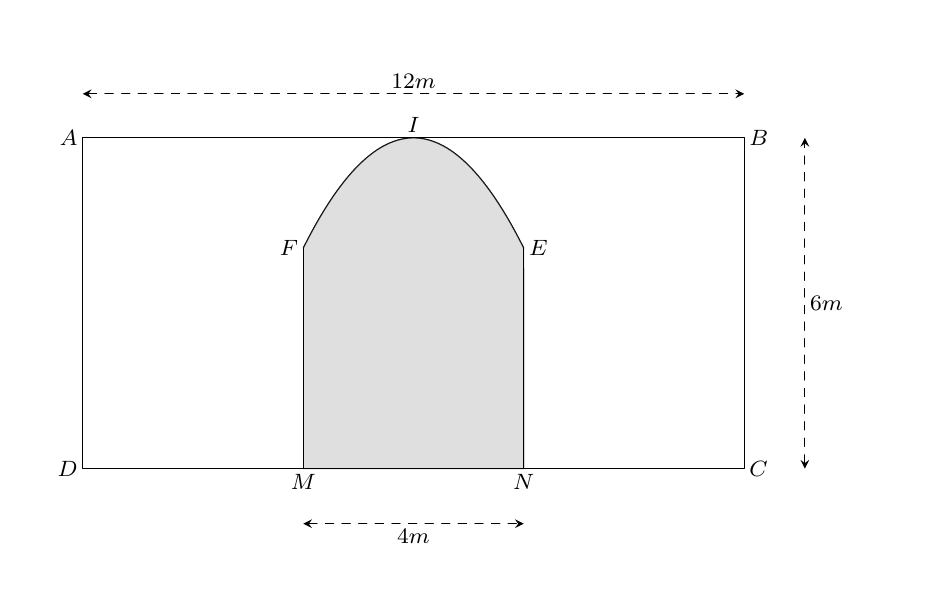
\begin{tikzpicture}[scale=.7,>=stealth,line cap=round,line join=round,font=\footnotesize]
				\def\f  (#1){-0.5*(#1)^2+6}
				\def\g (#1){0} 
				\def\xmin{-7} 
				 \def\xmax{9}
				 \def\ymin{-2}
				 \def\ymax{8}

				\clip  (\xmin,\ymin) rectangle (\xmax,\ymax);

				\draw[smooth,samples=200] plot[domain=2:-2]  (\x,{\f (\x)});
				\draw[smooth,samples=200]  plot[domain=2:-2] (\x,{\g (\x)});
				\draw[fill=gray!50!white,opacity=0.5]  plot[domain=-2:2] (\x,{\f (\x)})--plot[domain=2:-2](\x,{\g (\x)});
				\draw (-6,6)  node[left]{$A$}
					(6,6)  node[right]{$B$}
					(-6,0)  node[left]{$D$}
					(6,0) node[right]{$C$} 
					 (-2,4) node[left]{$F$}
					 (2,4) node[right]{$E$}
					 (-2,0) node[below]{$M$}
					(2,0)  node[below]{$N$}
					(0,-1)  node[below]{$4m$}
					 (7.1,3) node[right]{$6m$}
					(0,6.8) node[above]{$12m$} 
					 (0,6) node[above]{$I$};

					 (7,0)--(7,10)--(0,10);
				\draw (-6,6)--(6,6)--(6,0)--(-6,0)--cycle (2,0)--(2,4) 
					 (-2,0)--(-2,4);
				 \draw[<->,dashed] (-2,-1)--(2,-1);
				\draw[<->,dashed] (7.1,0)--(7.1,6); 
				\draw[<->,dashed] (-6,6.8)--(6,6.8); 
			\end{tikzpicture}
	\end{center}
	Biết $MN = 4m$;  cung $EIF$ có hình parabol với đỉnh $I$ là trung điểm của cạnh $AB$ và đi qua hai điểm $C, D$. Kinh phí làm bức tranh là $1.200.000$ đồng/m$^2$. Hỏi công ty đó cần bao nhiêu tiền để làm bức tranh?
	 \choice
		{$34\,266\,666$ đồng} 
		 {$13\,866\,666$ đồng}
		{$14\,933\,333$ đồng} 
		{\True  $27\,733\,333$ đồng }
	 \loigiai{
		Gọi $O$ là trung điểm cạnh $MN$ và trùng với gốc toạ độ  $\Rightarrow M(-2;0); N(2;0)$.\\
		Phương trình parabol đỉnh $I(0;6)$  và đi qua hai điểm $D(-6;0); C(6;0)$ là $(P): y = -\dfrac{1}{2}x^2 + 6$.\\
		Diện tích giới hạn bởi $(P): y =  -\dfrac{1}{2}x^2 + 6$; $y = 0$; $x = -2$; $x = 2$.\\
		Khi đó $S = \displaystyle\int_{-2}^{2} \left|  -\dfrac{1}{2}x^2 + 6 \right| \mathrm{\,d}x = \dfrac{208}{9} \text{ (m}^2)$.\\
		Vậy số tiền công  ty đó cần để làm bức tranh là $\dfrac{208}{9}\cdot1\cdot200\cdot000 = 27\,733\,333$ đồng.
	} 
\end{ex}

% nguồn: Phan1_Lop_12_Dai_so_Chuong_4
\begin{ex}%[2D4H3-1]%[ma:22279c3d]
	Hình bên dưới là mặt cắt dọc của một chiếc cầu bê tông (phần tô đậm, các đơn vị đều  đo bằng mét)
	\begin{center}
		\begin{tikzpicture}[scale=.7,xscale=.4,>=stealth,line cap=round,line join=round,font=\footnotesize]
				\def\f  (#1){-0.01*((#1)^2)+4}
				 \def\g (#1){5}
				\def\xmin{-22} 
				 \def\xmax{22}
				 \def\ymin{-1}
				\def\ymax{6} 
				\clip  (\xmin,\ymin) rectangle (\xmax+1.3,\ymax+1.3);
				\draw[->] (\xmin-1,0)--(\xmax+1,0) node[below]  {$x$};
				\draw[->] (0,\ymin-1)--(0,\ymax+1) node[left]  {$y$};
				\draw (0,0) node  [below left] {$O$};
				\draw[smooth,samples=200] plot[domain=-20:20] (\x,{\f  (\x)});
				\draw[smooth,samples=200] plot[domain=-20:20] (\x,{\g (\x)}); 
				\draw[fill=gray!50!white,opacity=0.5] plot[domain=-20:20] (\x,{\g  (\x)})--plot[domain=20:-20](\x,{\f (\x)});
				\draw  (20,0) node[below]{$A$};
				\draw  (-20,0) node[below]{$B$};
				\draw (0,5) node[above left]{$5$}; 
				\draw  (10,1.5) node[above left]{$y=4-\dfrac{x^2}{100}$};
				\draw (-20,0)--(-20,5) 
					 (20,0)--(20,5);
				\draw[->]  (5,3.75)--(6,2.5);
			\end{tikzpicture}
	\end{center}
	 Biết chiều rộng của cầu bằng 9m. Thể tích bê tông ít nhất cần để đúc cầu là
	 \choice
		{$760 \text{  m}^3$}
		{$780  \text{ m}^3$}
		 {$960 \text{ m}^3$}
		{\True $840  \text{ m}^3$}
	\loigiai{ 
		Parabol $y = 4 -  \dfrac{x^2}{100}$ cắt trục hoành tại hai điểm $A, B$.\\
		Cho $y = 0 \Rightarrow 4 - \dfrac{x^2}{100} = 0 \Rightarrow \begin{cases} x = 20 \\ x = -20
	\end{cases}$.\\
	 Do đó $A(-20;0)$ và $B(20;0)$.\\
	Diện tích hình phẳng  giới hạn bởi Parapol và trục hoành là $S = \displaystyle\int_{-20}^{20} \left( 4 - \dfrac{x^2}{100} \right) \mathrm{\,d}x = \dfrac{320}{3} \text{ (m}^2)$.\\
	Diện tích phần tô đậm bằng $40\cdot5 - \dfrac{320}{3} =  \dfrac{280}{3} \text{ (m}^2)$.\\
	Khi đó thể tích bê tông ít nhất cần để đúc cầu  là $\dfrac{280}{3}\cdot9 = 840 \text{ (m}^3)$.
 }
\end{ex}

% nguồn: Phan1_Lop_12_Dai_so_Chuong_4
\begin{ex}%[2D4H3-1]%[ma:4e10ef0b]
	Diện tích hình phẳng giới hạn bởi đồ thị của các hàm  số $y=x^2$, $y=x$ và các đường thẳng $x=0$, $x=1$ bằng
	 \choice
		{$\displaystyle\int_{-1}^0\left|x^2-x\right|\mathrm{\,d}x$} 
		 {$\displaystyle\int_0^1\left|x^2+x\right|\mathrm{\,d}x$}
		 {$\displaystyle\int_{-1}^0\left|x^2+x\right|\mathrm{\,d}x$}
		{\True $\displaystyle\int_0^1\left|x^2-x\right|\mathrm{\,d}x$} 
	\loigiai{ 
		 Phương trình hoành độ giao điểm $x^2=x\Leftrightarrow
		 \hoac{& x=0\\
		 & x=1.}$\\
	Suy  ra $S=\displaystyle\int_0^1\left|x^2-x\right|\mathrm{\,d}x$.}
\end{ex}

% nguồn: Phan1_Lop_12_Dai_so_Chuong_4
\begin{ex}%[2D4H3-1]%[ma:6d98d2bf]
	Diện tích hình  phẳng giới hạn bởi hai đồ thị hàm số $y = x^2 - 4x + 3$ và $y = x - 1$ bằng
	 \choice
		 {$\dfrac{3}{2}$}
		{\True  $\dfrac{9}{2}$}
		 {$1$}
		 {$-\dfrac{9}{2}$}
	 \loigiai{
		Xét phương trình: $x^2 - 4x + 3 = x - 1 \Leftrightarrow x^2 - 5x + 4 = 0 \Leftrightarrow \begin{cases} x = 1 \\ x = 4
	\end{cases}$.\\
	Suy ra, diện tích hình phẳng đã cho bằng\\ 
	$\displaystyle\int_{1}^{4} |(x^2 - 4x + 3) - (x - 1)| \mathrm{\,d}x = \displaystyle\int_{1}^{4} |x^2 - 5x  + 4| \mathrm{\,d}x = \displaystyle\int_{1}^{4} (-x^2 + 5x - 4) \mathrm{\,d}x = \dfrac{9}{2}$.
} 
\end{ex}

% nguồn: Phan1_Lop_12_Dai_so_Chuong_4
\begin{ex}%[2D4H3-1]%[ma:cacbca24]
	Diện tích hình phẳng giớn hạn bởi các đường $ y=x^2-4x+3$; $ x=0$ và $ y=0$  bằng
	\choice 
		 {$\dfrac{5}{3}$}
		{$\dfrac{16}{9}$} 
		 {$\dfrac{4}{3}$}
		{\True $\dfrac{8}{3}$} 
	\loigiai{ 
		Phương  trình hoành độ giao điểm: $x^2-4x+3=0\Leftrightarrow
		 \hoac{
		&  x=1\\
		 & x=3.}$\\
		\begin{center}
			$\begin{aligned}
			 & S=\displaystyle\int_0^3\left|x^2-4x+3\right|\mathrm{\,d}x=\displaystyle\int_0^1\left(x^2-4x+3\right)\mathrm{\,d}x-\displaystyle\int_1^3\left(x^2-4x+3\right)\mathrm{\,d}x\\
			 &=\left.\left(\dfrac{x^3}{3}-2x^2+3x\right)\right|_0^1-\left.\left(\dfrac{x^3}{3}-2x^2+3x\right)\right|_1^3=\dfrac{8}{3}.
		\end{aligned}$
\end{center}}
\end{ex}

% nguồn: Phan1_Lop_12_Dai_so_Chuong_4
\begin{ex}%[2D4H3-1]%[ma:06496f57]
	Diện tích hình phẳng giới hạn bởi đồ thị hàm số $y=\left(x-2\right)^2-1$, trục hoành và hai đường thẳng  $x=1$, $x=2$ bằng
	\choice 
		{\True $\dfrac{2}{3}$} 
		 {$\dfrac{7}{3}$}
		{$\dfrac{1}{3}$} 
		{$\dfrac{3}{2}$} 
	 \loigiai{
	Ta có $S=\displaystyle\int_1^2\left|\left(x-2\right)^2-1\right|\mathrm{\,d}x=\dfrac{2}{3}$.} 
\end{ex}

% nguồn: Phan1_Lop_12_Dai_so_Chuong_4
\begin{ex}%[2D4H3-1]%[ma:fbd2e852]
	Cho hàm số $y=f(x)$ liên tục trên đoạn $[a;b]$ có đồ thị như hình bên và $c\in[a;b]$. Gọi $S$ là diện tích của hình phẳng $(H)$ giới hạn bởi đồ thị hàm số $y=f(x)$ và các đường thẳng $y=0$, $x=a$, $x=b$. Mệnh đề nào sau đây \textbf{sai}? 
	\begin{center}
		\begin{tikzpicture}
				\draw[-stealth]  (-1.5,0)--(6,0) node[below]{$x$};
				\draw[-stealth]  (0,-4.5)--(0,2.5) node[left]{$y$};
				\draw (7pt,0)|-(0,7pt) 
					 (225:10pt) node {$O$};
				 \path (-0.5,-0.5) coordinate (A)
					(0,-1.5) coordinate (B) 
					(2,1.25)  coordinate (C)
					(4,0)  coordinate (D)
					(5,-4)  coordinate (E)
					(5.5,-2.5) coordinate  (F);
				 \def\duongcong{
					(A)..controls  +(-75:.25) and +(180:.25)..(B)
					..controls +(0:.45) and  +(180:1)..(C)
					..controls +(0:1) and  +(180:.85)..(E)
					..controls +(20:.38)  and +(-75:.05)..(F)
				} 
				\begin{scope}
					\clip (-0.5,0)--\duongcong--(5.5,0)--cycle; 
					\fill[pattern=north west lines](1.5,4) rectangle (4,-5); 
					\draw (1.5,0)--(1.5,2) 
						 (4,0)--(4,-4);
				\end{scope}
				\draw[red]  \duongcong;
				\draw (1.5,0) node[below]{$a$} 
					 (3,0) node[above right]{$c$}
					 (4,0) node[above right]{$b$};
			\end{tikzpicture}
	\end{center}
	 \choice
		 {\True $S=\displaystyle\int_a^c f(x)\,\mathrm{d}x+\displaystyle\int_c^b f(x)\,\mathrm{d}x$}
		{$S=\displaystyle\int_a^c f(x)\,\mathrm{d}x-\displaystyle\int_c^b f(x)\,\mathrm{d}x$} 
		{$S=\displaystyle\int_a^b\left|f(x)\right|\,\mathrm{d}x$} 
		{$S=\displaystyle\int_a^c f(x)\,\mathrm{d}x+\displaystyle\int_b^c f(x)\,\mathrm{d}x$} 
	\loigiai{Ta có $S=\displaystyle\int_a^b  \left| f(x)\right|\,\mathrm{d}x=\displaystyle\int_a^c f(x)\,\mathrm{d}x-\displaystyle\int_c^b f(x)\,\mathrm{d}x=\displaystyle\int_a^c f(x)\,\mathrm{d}x+\displaystyle\int_b^c f(x)\,\mathrm{d}x$.}
\end{ex}

% nguồn: Phan1_Lop_12_Dai_so_Chuong_4
\begin{ex}%[2D4H3-1]%[ma:b13b1db8]
	Cho hàm số $y = f(x) = 2x^3 + ax^2 + bx (a,b \in \mathbb{R})$. Biết hàm số $y = f'(x)$ có đồ thị như  hình vẽ
	\begin{center}
		\begin{tikzpicture}[scale=1.7,yscale=.4,>=stealth,line cap=round,line join=round,font=\footnotesize]
				 \def\f (#1){6*(#1)^2-8*(#1)}
				\def\xmin{-1} 
				 \def\xmax{2}
				 \def\ymin{-3}
				 \def\ymax{2}
				\clip (\xmin,\ymin) rectangle  (\xmax,\ymax);
				 \draw[->] (\xmin-1,0)--(\xmax,0) node[below left] {$x$};
				 \draw[->] (0,\ymin-1)--(0,\ymax) node[below right] {$y$};
				\draw (0,0)  node [above right] {$O$};
				\draw[smooth,samples=200]  plot[domain=\xmin:\xmax] (\x,{\f (\x)});
				 \draw (1.334,0) node[below right]{$\dfrac{4}{3}$};
			\end{tikzpicture}
	\end{center}
	Diện tích của hình phẳng giới hạn bởi đồ thị $y = f(x)$ và $y = f'(x)$ bằng $\dfrac{m}{n} (m \in \mathbb{Z}, n \in \mathbb{N}^*)$ và $\dfrac{m}{n}$  là phân số tối giản. Tính $m + n$.
	 \choice
		 {$-157$}
		 {\True $74$}
		{$13$} 
		{$119$} 
	\loigiai{ 
		 Ta có $f'(x) = 6x^2 + 2ax + b$.\\
		Từ đồ thị suy ra $\begin{cases} f'(0) = 0 \\ f'(\dfrac{4}{3}) = 0
	\end{cases} \Rightarrow \begin{cases} b = 0 \\ a = -4.
	\end{cases}$\\
	Ta  có $f(x) - f'(x) = 2x^3 + (-4)x^2 + 0x - (6x^2 + 2(-4)x + 0) = 2x^3 - 10x^2 + 8x$.\\
	Cho $f(x) - f'(x) = 0 \Leftrightarrow 2x^3 - 10x^2 + 8x = 0 \Leftrightarrow \begin{cases} x = 0 \\ x = 1 \\ x = 4
	\end{cases}$.
	Vậy diện tích hình phẳng $S = \displaystyle\int_{0}^{4} |2x^3  - 10x^2 + 8x| \mathrm{\,d}x = \dfrac{71}{3}$.\\
	Suy ra $m = 71$, $n = 3$. 
	Vậy $m + n  = 71 + 3 = 74$.
} 
\end{ex}

% nguồn: Phan1_Lop_12_Dai_so_Chuong_4
\begin{ex}%[2D4H3-1]%[ma:93a334ed]
	Bác An có mảnh vườn hình chữ nhật $ABCD$, chiều dài $AB = 2\pi\, (m)$, chiều rộng $BC = 3\, (m)$. Bác muốn trồng hoa trên dải đất (phần tô đậm) được giới hạn bởi đường $MN$ (với $M,N$ lần lượt là trung điểm của $AD, BC$)  và một đường hình sin (tham khảo hình vẽ). Diện tích đất trồng hoa bằng.
	\begin{center}
		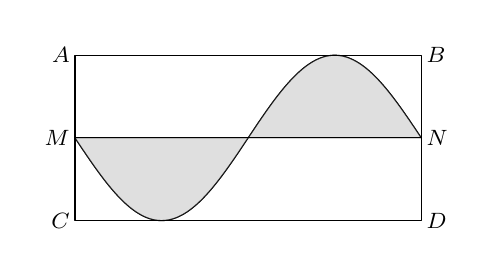
\begin{tikzpicture}[scale=.7,>=stealth,line cap=round,line join=round,font=\footnotesize]
				\def\xmin{-4} 
				 \def\xmax{4}
				\def\ymin{-2} 
				 \def\ymax{2}
				\clip (\xmin,\ymin)  rectangle (\xmax,\ymax);
				\draw[smooth,samples=200] plot[domain=-3.142:3.142] (\x,{1.5*sin (\x  r)});
				\draw[fill=gray!50!white,opacity=0.5] plot[domain=-3.142:3.142] (\x,{1.5*sin (\x r)})--plot[domain=3.142:-3.142](\x,{0}); 
				\draw (-3.142,1.5)  node[left]{$A$}
					(3.142,1.5) node[right]{$B$} 
					(3.142,-1.5) node[right]{$D$} 
					(-3.142,-1.5) node[left]{$C$} 
					(-3.142,0)  node[left]{$M$}
					 (3.142,0) node[right]{$N$};
				\draw  (-3.142,1.5)--(3.142,1.5)--(3.142,-1.5)--(-3.142,-1.5)--cycle (-3.142,0)--(3.142,0);
			\end{tikzpicture}
	\end{center}
	 \choice
		{$3\,m^2$} 
		 {$5,57\,m^2$}
		{$7,14\,m^2$} 
		{\True  $6\,m^2$}
	 \loigiai{
		Dựng hệ trục tọa độ $Oxy$ như hình  vẽ.
		\begin{center}
			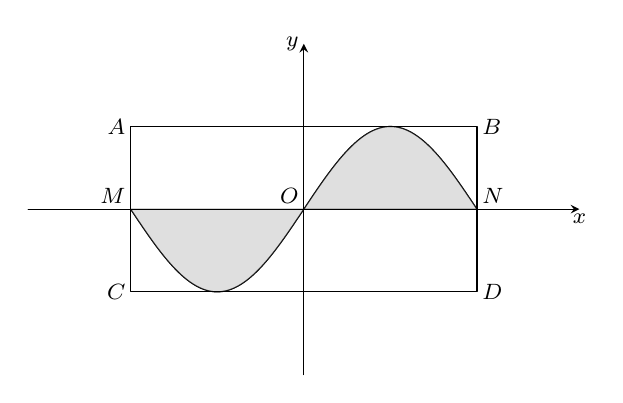
\begin{tikzpicture}[scale=.7,>=stealth,line cap=round,line join=round,font=\footnotesize]
					 \def\xmin{-4}
					 \def\xmax{4}
					 \def\ymin{-2}
					\def\ymax{2} 
					\draw[->] (\xmin-1,0)--(\xmax+1,0) node[below] {$x$}; 
					\draw[->] (0,\ymin-1)--(0,\ymax+1)  node[left] {$y$};
					\draw  (0,0) node [above left] {$O$};
					\clip (\xmin,\ymin)  rectangle (\xmax,\ymax);
					\draw[smooth,samples=200] plot[domain=-3.142:3.142] (\x,{1.5*sin (\x  r)});
					\draw[fill=gray!50!white,opacity=0.5] plot[domain=-3.142:3.142] (\x,{1.5*sin  (\x r)})--plot[domain=3.142:-3.142](\x,{0});
					\draw  (-3.142,1.5) node[left]{$A$}
						(3.142,1.5)  node[right]{$B$}
						(3.142,-1.5)  node[right]{$D$}
						(-3.142,-1.5) node[left]{$C$} 
						(-3.142,0)  node[above left]{$M$}
						(3.142,0) node[above right]{$N$}; 
					\draw (-3.142,1.5)--(3.142,1.5)--(3.142,-1.5)--(-3.142,-1.5)--cycle (-3.142,0)--(3.142,0); 
				\end{tikzpicture}
		\end{center}
		Vì phần đường cong là một đồ thị hình  sin đi qua các điểm $(0;0)$, $\left(-\dfrac{\pi}{2}; 1{,}5 \right)$, $(-\pi;0)$, $\left(\dfrac{\pi}{2}; 1{,}5 \right)$, $(\pi; 0)$ nên đường cong có phương trình $y = \dfrac{3}{2} \sin x$.\\
		Khi đó phần diện tích đất trồng hoa giới hạn bởi các đồ thị hàm  số
		$ \left\{ 
		\begin{aligned}
			&y = \dfrac{3}{2} \sin  x \\
			&y = 0  \\
			&x  = -\pi,\; x = \pi
		\end{aligned}
		 \right.$\\
		 Do đó diện tích đất trồng hoa là
		$ 
		S = \displaystyle\int_{-\pi}^{\pi} \left| \dfrac{3}{2} \sin x \right| \, \mathrm{\,d}x = 6 \text{ m}^2. 
		$ 
		 }
\end{ex}

% nguồn: Phan1_Lop_12_Dai_so_Chuong_4
\begin{ex}%[2D4H3-1]%[ma:b29f4545]
	Một biển quảng cáo có dạng hình vuông $ABCD$ cạnh $AB = 4m$. Trên tâm biển đó có các đường tròn tâm $A$ và đường  tròn tâm $B$ cùng bán kính $R = 4m$, hai đường tròn cắt nhau như hình vẽ. Chi phí để sơn phần gạch chéo là $150 \ 000$ đồng/m$^2$, chi phí sơn phần màu đen là $100 \ 000$ đồng/m$^2$ và chi phí để sơn phần còn lại là $250 \ 000$ đồng/m$^2$.
	\begin{center}
		\begin{tikzpicture}[scale=.7,>=stealth,line cap=round,line join=round,font=\footnotesize]
				 \def\n{.5}
				\def\xmin{-1} 
				\def\xmax{5} 
				\def\ymin{-1} 
				 \def\ymax{5}
				\clip (\xmin,\ymin) rectangle (\xmax,\ymax); 
				\draw[smooth,samples=200]  plot[domain=0:4] (\x,{((16-(\x)^2)^\n)});
				\draw[smooth,samples=200] plot[domain=0:4]  (\x,{((16-((\x)-4)^2)^\n)});
				\draw[fill=gray!50!white,opacity=0.5]  plot[domain=0:4] (\x,{((16-(\x)^2)^\n)})--plot[domain=4:0](\x,{((16-((\x)-4)^2)^\n)});
				\draw[pattern=north west lines,opacity=0.5] plot[domain=0:2]  (\x,{((16-((\x)-4)^2)^\n)})--plot[domain=2:0](\x,{0});
				\draw[pattern=north west  lines,opacity=0.5] plot[domain=2:4] (\x,{((16-(\x)^2)^\n)})--plot[domain=4:2](\x,{0});
				 \draw (0,0) node[left]{$A$}
					(4,0) node[right]{$B$} 
					(0,4)  node[left]{$D$}
					 (4,4) node[right]{$C$}
					(2,0)  node[below]{$4m$}
					(4,2)  node[right]{$4m$};
				\draw  (0,0)--(0,4)--(4,4)--(4,0)--cycle;
			\end{tikzpicture}
	\end{center}
	Hỏi số tiền  để sơn biển quảng cáo theo cách trên gần nhất với số tiền nào dưới đây?
	\choice 
		{$3,017$ triệu  đồng }
		{$1,213$ triệu  đồng}
		 {$2,06$ triệu đồng}
		{\True $2,195$ triệu đồng} 
	\loigiai{ 
		Gọi $I$ là giao điểm  của 2 cung tròn $\wideparen{AC}, \wideparen{BD}$. Chọn gốc tọa độ $A(0;0) \Rightarrow B(4,0)$.\\
		Xét cung tròn có phương trình $y =  \sqrt{16 - x^2}$.\\
		Phần diện tích gạch  chéo
		$ S = 2 \displaystyle\int_{0}^{4} \sqrt{16 - x^2}  \, \mathrm{\,d}x = 16 \left( x + \dfrac{1}{2} \sin 2x \right) \bigg|_{0}^{\tfrac{\pi}{6}} = \dfrac{16\pi}{3} - 4\sqrt{3}$.\\
		 Phần diện tích màu đen:
		$ 2 \cdot \left(  \dfrac{1}{4} \pi \cdot 4^2 - \dfrac{16\pi}{3} + 4\sqrt{3} \right) = \dfrac{-8\pi}{3} + 8\sqrt{3}.$\\
		Phần diện  tích còn lại:
		$16 - \left( \dfrac{16\pi}{3} - 4\sqrt{3} + \dfrac{-8\pi}{3} + 8\sqrt{3} \right) = 16 - \left( \dfrac{8\pi}{3} - 4\sqrt{3} \right) $.\\ 
		Số  tiền để sơn biển quảng cáo:
		$\left( \dfrac{16\pi}{3} - 4\sqrt{3} \right) \cdot 150~000 + \left( \dfrac{-8\pi}{3} + 8\sqrt{3} \right) \cdot 100~000 + \left( 16 - \dfrac{8\pi}{3} + 4\sqrt{3} \right) \cdot 250~000 = 2{,}195~\text{  triệu đồng}.$
	} 
\end{ex}

% nguồn: Phan1_Lop_12_Dai_so_Chuong_4
\begin{ex}%[2D4H3-1]%[ma:34b8c743]
	 Một hoa văn hình tròn tâm $O$, ngoại tiếp tam giác đều $ABC$ có cạnh $AB = 4\sqrt{3} \text{ cm}$. Đường cong qua ba điểm $A$, $B$, $C$ là một phần của parabol.
	\begin{center}
		\begin{tikzpicture}[scale=.7,>=stealth,line cap=round,line join=round,font=\footnotesize]
				\def\a{-0.5} 
				\def\b{4} 
				 \def\c{2}
				 \def\d{0}
				 \def\f (#1){\a*((#1)^2)+\b}
				\def\m{-1} 
				\def\n{0.5} 
				 \def\p{8}
				 \def\q{0}
				\def\xmin{-5} 
				\def\xmax{4} 
				\def\ymin{-5} 
				 \def\ymax{4}
				 \clip (\xmin,\ymin) rectangle (\xmax+1.3,\ymax+1.3);
				 \draw (0,0) node [left] {$O$};
				 \draw[smooth,samples=200] plot[domain=-3.46:3.46] (\x,{\f (\x)});
				\draw[smooth,samples=200] plot[domain=-3.46:3.46]  (\x,{\m*((16-(\x)^2)^\n)});
				\draw[pattern=north west lines,opacity=0.5] plot[domain=-3.46:3.46]  (\x,{\m*((16-(\x)^2)^\n)})--plot[domain=3.46:-3.46](\x,{\f (\x)});
				 \draw (-3.46,-2) node[left]{$A$};
				 \draw (3.46,-2) node[right]{$B$};
				\draw  (0,-2) node[below]{$D$};
				\draw (0,4)  node[above]{$C$};
				\draw (-3.46,-2)--(3.46,-2) 
					 (0,4)--(0,-2);
				\draw (0,0)  circle (4);
				\fill (0,0)  circle (2pt);
			\end{tikzpicture}
	\end{center}
	Diện  tích phần gạch chéo bằng
	 \choice
		{\True  $37,54 \text{ cm}^2$}
		{$9,83 \text{ cm}^2$} 
		{$27,71 \text{ cm}^2$} 
		{$36,75  \text{ cm}^2$}
	 \loigiai{
		\begin{center}
			\begin{tikzpicture}[scale=.7,>=stealth,line cap=round,line join=round,font=\footnotesize]
					\def\a{-0.5} 
					 \def\b{4}
					 \def\c{2}
					 \def\d{0}
					\def\f  (#1){\a*((#1)^2)+\b}
					\def\m{-1} 
					 \def\n{0.5}
					 \def\p{8}
					 \def\q{0}
					 \def\xmin{-5}
					\def\xmax{4} 
					 \def\ymin{-5}
					 \def\ymax{4}
					 \clip (\xmin,\ymin) rectangle (\xmax+1.3,\ymax+1.3);
					\draw[->] (\xmin-1,0)--(\xmax+1,0)  node[below] {$x$};
					\draw[->]  (0,\ymin-1)--(0,\ymax+1) node[left] {$y$};
					\draw (0,0) node [below left] {$O$}; 
					 \draw[smooth,samples=200] plot[domain=-3.46:3.46] (\x,{\f (\x)});
					\draw[smooth,samples=200]  plot[domain=-3.46:3.46] (\x,{\m*((16-(\x)^2)^\n)});
					 \draw[pattern=north west lines,opacity=0.5] plot[domain=-3.46:3.46] (\x,{\m*((16-(\x)^2)^\n)})--plot[domain=3.46:-3.46](\x,{\f (\x)});
					\draw (-3.46,-2) node[left]{$A$}; 
					 \draw (3.46,-2) node[right]{$B$};
					 \draw (0,-2) node[above right]{$D$};
					\draw  (0,4) node[above right]{$C$};
					\draw (-3.46,-2)--(3.46,-2); 
					\draw (0,0) circle (4); 
				\end{tikzpicture}
		\end{center}
		Do tam giác $ABC$ là tam giác đều có cạnh $4\sqrt{3} \text{ cm}$ nên  ta có
		$CD = 4\sqrt{3}.\dfrac{\sqrt{3}}{2} = 6 \text{ (cm)} \Rightarrow OC = \dfrac{2}{3}CD = 4 \text{ (cm)}$ và $OD = 2 \text{  (cm)}$.\\
		Gắn trục toạ độ $Oxy$ như hình vẽ, ta có: $A(-2\sqrt{3};-2)$, $B(2\sqrt{3};-2)$,  $C(0;4)$.\\
		Phương trình đường Parabol đi qua $3$ điểm $A$, $B$, $C$ có đỉnh  $C$ có dạng $y = ax^2 + 4 \,(P)$.\\
		Thay toạ độ điểm $B(2\sqrt{3};-2)$ vào $(P)$ suy ra $a = -\dfrac{1}{2} \Rightarrow  (P): y = -\dfrac{1}{2}x^2 + 4$.\\
		Phương trình đường tròn tâm $O$ bán kính $OA = 4$ là $x^2 + y^2 = 16$.\\ 
		 Phương trình một phần cung nhỏ $AB$ có dạng $y = -\sqrt{16 - x^2}$.\\
		Vậy diện tích phần gạch chéo bằng $\displaystyle\int_{-2\sqrt{3}}^{2\sqrt{3}} \left[\left(-\dfrac{1}{2}x^2 + 4\right) - \left(-\sqrt{16 - x^2}\right) \right] \mathrm{\,d}x \approx 37,54  \text{ (cm}^2)$.
	} 
\end{ex}

% nguồn: Phan1_Lop_12_Dai_so_Chuong_4
\begin{ex}%[2D4H3-1]%[ma:fb562686]
	Diện tích  phần sạch sọc trong hình vẽ bằng
	\begin{center}
		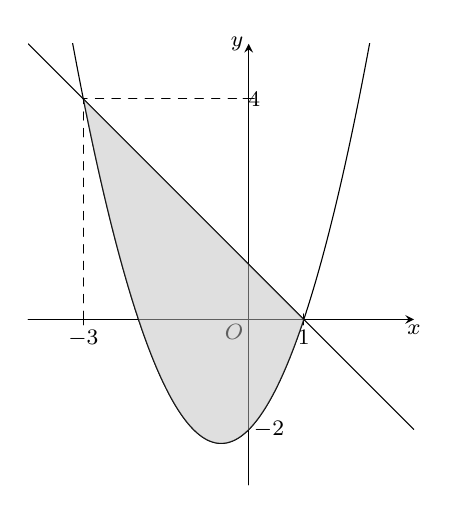
\begin{tikzpicture}[scale=.7,>=stealth,line cap=round,line join=round,font=\footnotesize]
				 \def\a{1}
				 \def\b{1}
				 \def\c{-2}
				 \def\d{0}
				 \def\f (#1){\a*((#1)^2)+\b*((#1))+\c}
				 \def\xmin{-4}
				\def\xmax{3} 
				 \def\ymin{-3}
				\def\ymax{5} 
				\draw[->] (\xmin,0)--(\xmax,0)  node[below] {$x$};
				\draw[->] (0,\ymin)--(0,\ymax) node[left] {$y$}; 
				\draw (0,0) node [below left]  {$O$};
				\clip (\xmin,\ymin) rectangle  (\xmax,\ymax);
				\foreach \x  in {-3,1}\draw (\x,0.1)--(\x,-0.1) node [below] {$\x$};
				\foreach \y in {4}\draw (0.1,\y)--(-0.1,\y) node  [right] {$\y$};
				\draw[smooth,samples=200] plot[domain=\xmin:\xmax] (\x,{\f  (\x)});
				\draw[smooth,samples=200] plot[domain=\xmin:\xmax] (\x,{-\x+1}); 
				\draw[fill=gray!50!white,opacity=0.5] plot[domain=-3:1] (\x,{\f (\x)})--plot[domain=-3:1](\x,{-(\x)+1}); 
				 \draw (0,-2) node[right]{$-2$};
				\draw[dashed]  (-3,0)--(-3,4)--(0,4);
			\end{tikzpicture}
	\end{center}
	\choice 
		{$\displaystyle\int_{-3}^{1} |-x^2 - 2x  - 3| \mathrm{\,d}x$}
		{$\displaystyle\int_{-3}^{1} (x^2 - 2x  - 3) \mathrm{\,d}x$}
		 {$\displaystyle\int_{-3}^{1} (x^2 + 2x - 3) \mathrm{\,d}x$}
		{\True $\displaystyle\int_{-3}^{1} (-x^2 -  2x + 3) \mathrm{\,d}x$}
	 \loigiai{
		Dựa vào  đồ thị hai hàm số $y = x^2 + x - 2$ và $y = -x + 1$.\\
		Ta có diện  tích hình phẳng là $S = \displaystyle\int_{-3}^{1} (-x + 1 - (x^2 + x - 2)) \mathrm{\,d}x = \displaystyle\int_{-3}^{1} (-x^2 - 2x + 3) \mathrm{\,d}x$.
	 }
\end{ex}

% nguồn: Phan1_Lop_12_Dai_so_Chuong_4
\begin{ex}%[2D4H3-1]%[ma:abccf5f6]
	Diện tích hình phẳng phần gạch chéo trong hình vẽ bên được tính  theo công thức nào sau đây?
	\begin{center}
		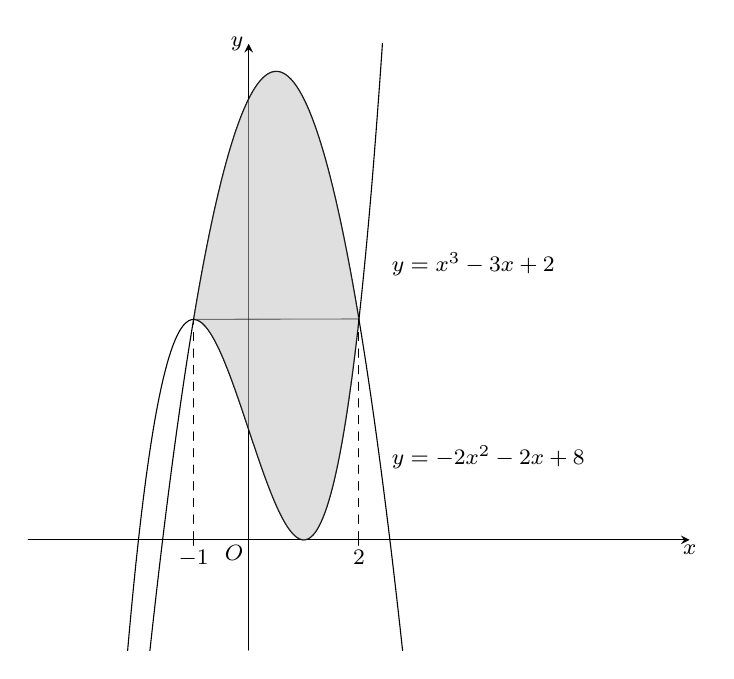
\begin{tikzpicture}[scale=.7,>=stealth,line cap=round,line join=round,font=\footnotesize]
				\def\a{1} 
				 \def\b{-3}
				 \def\c{2}
				 \def\d{0}
				\def\f  (#1){\a*((#1)^3)+\b*((#1))+\c}
				 \def\m{-2}
				\def\n{2} 
				\def\p{8} 
				 \def\q{0}
				\def\g (#1){\m*((#1)^2)+\n*((#1))+\p} 
				 \def\xmin{-3}
				 \def\xmax{7}
				\def\ymin{-2} 
				\def\ymax{9} 
				\draw[->]  (\xmin-1,0)--(\xmax+1,0) node[below] {$x$};
				\draw[->]  (0,\ymin)--(0,\ymax) node[left] {$y$};
				\draw (0,0) node [below  left] {$O$};
				 \clip (\xmin,\ymin) rectangle (\xmax,\ymax);
				\foreach \x in {-1,2}\draw (\x,0.1)--(\x,-0.1) node  [below] {$\x$};
				\draw[smooth,samples=200] plot[domain=\xmin:\xmax]  (\x,{\f (\x)});
				\draw[smooth,samples=200]  plot[domain=\xmin:\xmax] (\x,{\g (\x)});
				\draw[fill=gray!50!white,opacity=0.5]  plot[domain=-1:2] (\x,{\g (\x)})--plot[domain=-1:2](\x,{\f (\x)});
				\draw (2.5,5) node[right]{$y=x^3-3x+2$}; 
				 \draw (2.5,1.5) node[right]{$y=-2x^2-2x+8$};
				\draw[dashed] (-1,0)--(-1,4) 
					(2,0)--(2,4); 
			\end{tikzpicture}
	\end{center}
	 \choice
		{$S = \displaystyle\int_{-1}^{2} (x^3 + 2x^2  - 5x - 6) \mathrm{\,d}x$}
		{$S = \displaystyle\int_{-1}^{2} (x^3 + 2x^2 -  x - 10) \mathrm{\,d}x$}
		{$S = \displaystyle\int_{-1}^{2} (x^3 - 2x^2 -  x + 10) \mathrm{\,d}x$}
		{\True  $S = \displaystyle\int_{-1}^{2} (-x^3 - 2x^2 + 5x + 6) \mathrm{\,d}x$}
	\loigiai{ 
		Ta có:  $S = \displaystyle\int_{-1}^{2} |(x^3 - 3x + 2) - (-2x^2 + 2x + 8)| \mathrm{\,d}x = \displaystyle\int_{-1}^{2} [(-2x^2 + 2x + 8) - (x^3 - 3x + 2)] \mathrm{\,d}x$.\\
		Do $-2x^2 + 2x + 8  \ge x^3 - 3x + 2$, $\forall x \in [-1;2]$ nên $S = \displaystyle\int_{-1}^{2} (-x^3 - 2x^2 + 5x + 6) \mathrm{\,d}x$.\\
		Vậy diện tích hình phẳng phần gạch chéo trong hình vẽ là $S = \displaystyle\int_{-1}^{2} (-x^3 - 2x^2 + 5x  + 6) \mathrm{\,d}x$.
	 }
\end{ex}

% nguồn: Phan1_Lop_12_Dai_so_Chuong_4
\begin{ex}%[2D4H3-1]%[ma:a436d10d]
	Cho hàm số $y = f(x)$  có tập xác định là $[-3;3]$ và có đồ thị như hình vẽ. Giá trị của $\displaystyle\int_{-3}^{3} f(x) \mathrm{\,d}x$ bằng
	\begin{center}
		\begin{tikzpicture}[scale=.9,>=stealth,line cap=round,line join=round,font=\footnotesize]
				 \def\xmin{-4}
				 \def\xmax{4}
				 \def\ymin{-2}
				 \def\ymax{5}
				\draw[->] (\xmin,0)--(\xmax,0) node[below] {$x$}; 
				 \draw[->] (0,\ymin)--(0,\ymax) node[left] {$y$};
				\draw  (0,0) node [below left] {$O$};
				 \clip (\xmin,\ymin) rectangle (\xmax,\ymax);
				\foreach \x  in {-3,-2}\draw (\x,0.1)--(\x,-0.1) node [above] {$\x$};
				\foreach \x in {-1,1,3}\draw  (\x,0.1)--(\x,-0.1) node [below] {$\x$};
				\foreach \y in {-1,1}\draw (0.1,\y)--(-0.1,\y)  node [right] {$\y$};
				\foreach \y  in {4}\draw (0.1,\y)--(-0.1,\y) node [left] {$\y$};
				\draw[dashed]  (-3,0)--(-3,-1)--(0,-1)
					 (-1,0)--(-1,1)--(0,1)
					 (3,0)--(3,4)--(0,4);
				 \draw (-3,-1)--(-1,1)--(1,0)--(3,4);
			\end{tikzpicture}
	\end{center}
	 \choice
		{$6$} 
		 {\True $5$}
		 {$12$}
		{$10$} 
	\loigiai{ 
		Ta  có
		\begin{eqnarray*}
			\displaystyle\int_{-3}^{3} f(x) \mathrm{\,d}x&= & \displaystyle\int_{-3}^{-2} f(x)  \mathrm{\,d}x + \displaystyle\int_{-2}^{1} f(x) \mathrm{\,d}x + \displaystyle\int_{1}^{3} f(x) \mathrm{\,d}x\\
			&= & -S_{\triangle  ABC} + S_{\triangle CDE} + S_{\triangle EFG}\\
			&= & -\dfrac{1}{2}\cdot1\cdot1 + \dfrac{1}{2}\cdot1\cdot3 + \dfrac{1}{2}\cdot2\cdot4 =  5.
		\end{eqnarray*}
	 }
\end{ex}

% nguồn: Phan1_Lop_12_Dai_so_Chuong_4
\begin{ex}%[2D4H3-1]%[ma:8a772ee0]
	Hình phẳng giới hạn bởi đồ thị hàm số $y=-x^2+2x$ và  trục $Ox$ có diện tích là
	\choice 
		{\True $\dfrac{4}{3}$} 
		{$\dfrac{2}{3}$} 
		 {$\dfrac{8}{3}$}
		 {$\dfrac{20}{3}$}
	 \loigiai{
		Ta có  $-x^2+2x=0 \Leftrightarrow \hoac{&x=0\\&x=2.}$\\
		 Diện tích
		\begin{align*}
			S &= \displaystyle \int_{0}^{2} |-x^2+2x|  \mathrm{\,d}x
			=\displaystyle \int_{0}^{2} \left(-x^2+2x\right)  \mathrm{\,d}x
			 =\left(-\dfrac{x^3}{3} + x^2\right)\bigg|_0^2
			=\dfrac{4}{3}. 
		\end{align*}
	 }
\end{ex}

% nguồn: Phan1_Lop_12_Dai_so_Chuong_4
\begin{ex}%[2D4H3-1]%[ma:657ffa3b]
	Cho hình $(H)$ là hình phẳng giới hạn bởi đường cong $y = x^3$, đường thẳng $y = -2x + 3$ và trục hoành (phần gạch chéo trong hình vẽ). Diện tích hình  phẳng $(H)$ là
	\begin{center}
		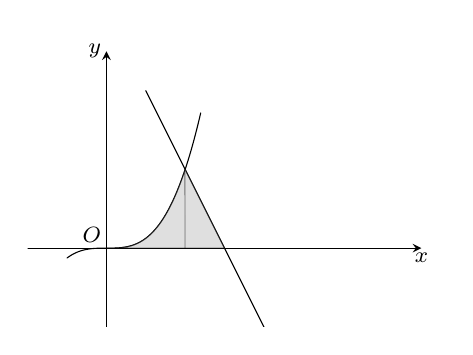
\begin{tikzpicture}[scale=1,>=stealth,line cap=round,line join=round,font=\footnotesize]
				 \def\a{1}
				 \def\f (#1){(#1)^3}
				 \def\m{-2}
				\def\g (#1){\m*(#1)+3} 
				\def\xmin{-1} 
				\def\xmax{3} 
				\def\ymin{-1} 
				 \def\ymax{1.5}
				\clip (\xmin,\ymin)  rectangle (\xmax+1.3,\ymax+1.3);
				 \draw[->] (\xmin-1,0)--(\xmax+1,0) node[below] {$x$};
				\draw[->] (0,\ymin-1)--(0,\ymax+1) node[left] {$y$}; 
				\draw (0,0) node [above left]  {$O$};
				\draw[smooth,samples=200] plot[domain=-0.5:1.2] (\x,{\f  (\x)});
				\draw[smooth,samples=200]  plot[domain=0.5:\xmax] (\x,{\g (\x)});
				 \draw[fill=gray!50!white,opacity=0.5] plot[domain=0:1] (\x,{\f (\x)})--plot[domain=1:0](\x,{0});
				\draw[fill=gray!50!white,opacity=0.5] plot[domain=1:1.5]  (\x,{\g (\x)})--plot[domain=1.5:1](\x,{0});
			\end{tikzpicture}
	\end{center}
	 \choice
		 {$S = \dfrac{1}{4}$}
		 {\True $S = \dfrac{1}{2}$}
		 {$S = \dfrac{5}{4}$}
		 {$S = 2$}
	\loigiai{ 
		Ta có $x^3 = -2x + 3 \Leftrightarrow x^3 + 2x - 3 =  0 \Leftrightarrow x = 1$.\\
		Đường cong $y = x^3$ đi qua $O(0;0)$ và  $y = -2x + 3$ cắt $Ox$ tại điểm có hoành độ $x = \dfrac{3}{2}$.\\
		Vậy $S = \displaystyle\int_{0}^{1} x^3 \mathrm{\,d}x + \displaystyle\int_{1}^{\tfrac{3}{2}} (-2x  + 3) \mathrm{\,d}x = \left. \dfrac{x^4}{4} \right|_{0}^{1} + \left. (3x - x^2) \right|_{1}^{\tfrac{3}{2}} = \dfrac{1}{2}$.
	 }
\end{ex}

% nguồn: Phan1_Lop_12_Dai_so_Chuong_4
\begin{ex}%[2D4H3-1]%[ma:a125ad63]
	 \immini[thm]{
	Cho hàm số $y=f(x)$ liên tục trên $\Bbb{R}$ và có đồ thị như hình vẽ. Gọi $S$ là diện  tích hình phẳng giới hạn bởi đồ thị hàm số $y=f(x)$, trục hoành và hai đường thẳng $x=-1$, $x=3$. Mệnh đề nào sau đây đúng?
	 }
	{ 
	\begin{tikzpicture}[scale=0.8,font=\footnotesize,line join=round,line cap=round,>=stealth]
			\tikzset{every  node/.style={scale=0.9}}
			\draw[->] (-3.1,0)--(5.1,0) node[below left]  {$x$};
			\draw[->] (0,-2.1)--(0,3.1) node[below left]  {$y$};
			 \draw (0,0) node [below right] {$O$};
			 \draw[dashed] (-1,-2)--(-1,3)
				 (3,-2)--(3,3);
			\draw (1.5,0) node [below]  {$\tfrac{3}{2}$} circle (1pt)
				(-2,0)  node [above left] {$-2$} circle (1pt)
				(-1,0) node  [below right] {$-1$} circle (1pt)
				(3,0) node [below right]  {$3$} circle (1pt)
				(4,0)  node [below] {$4$} circle (1pt);
			\begin{scope}
				\clip (-3,-3) rectangle (5,3); 
				\draw[name path=(C)] plot[smooth,tension=0.7] coordinates{(-2.5,-2) 
					 (-0.8,2)
					 (3,-1)
					 (5.1,3)};
			\end{scope}
		\end{tikzpicture}
	} 
	 \choice
		 {$S=\displaystyle\int_{-1}^3 f(x)\mathrm{\,d}x$}
		 {$S\left|=\displaystyle\int_{-1}^3 f(x)\mathrm{\,d}x\right|$}
		 {$S=\displaystyle\int_{-1}^{\tfrac{3}{2}}f(x)\mathrm{\,d}x+\displaystyle\int_{\tfrac{3}{2}}^3 f(x)\mathrm{\,d}x$}
		{\True $S=\displaystyle\int_{-1}^{\tfrac{3}{2}}f(x)\mathrm{\,d}x-\displaystyle\int_{\tfrac{3}{2}}^3  f(x)\mathrm{\,d}x$}
	 \loigiai{
		Ta có  $S=\displaystyle\int_{-1}^3 |f(x)|\mathrm{\,d}x=\displaystyle\int_{-1}^{\tfrac{3}{2}}f(x)\mathrm{\,d}x-\displaystyle\int_{\tfrac{3}{2}}^3 f(x)\mathrm{\,d}x$.
	} 
\end{ex}

% nguồn: Phan1_Lop_12_Dai_so_Chuong_4
\begin{ex}%[2D4H3-1]%[ma:797cacf5]
	Cho hàm số $y = f(x)$ liên tục trên $\mathbb{R}$. Gọi $F(x)$, $G(x)$ lần lượt là nguyên hàm của $f(x)$ và $f(x) - 2x - 1$ trên $\mathbb{R}$ thỏa mãn $F(2) +  2G(1) = 2023$; $2F(1) + G(2) = 2019$. Diện tích hình phẳng giới hạn bởi các đường $y = F(x)$ và $y = G(x)$ bằng
	 \choice
		{$\dfrac{31}{6}$} 
		{\True $\dfrac{9}{2}$} 
		 {$\dfrac{125}{6}$}
		{$\dfrac{15}{2}$} 
	\loigiai{ 
		Theo bài ra ta có $F'(x) =  f(x)$ và $G'(x) = f(x) - 2x - 1$ với $\forall x \in \mathbb{R}$.\\
		 Nên $F'(x) = G'(x) + 2x + 1 \Rightarrow F(x) = G(x) + x^2 + x + C$.\\
		Vì 
		\begin{eqnarray*}
			& & \begin{cases} F(2) + 2G(1) = 2023 \\ 2F(1) + G(2) = 2019
		\end{cases}\\
		&\Leftrightarrow & \begin{cases} G(2) + 2^2 + 2 + C + 2G(1) = 2023 \\ 2(G(1) + 1^2 + 1 + C) + G(2) = 2019
	\end{cases}\\
	&\Leftrightarrow &\begin{cases} G(2) + 2G(1) + 6 + C = 2023 \\ G(2) + 2G(1) + 4 + 2C = 2019
	\end{cases}
	\end{eqnarray*}
	Trừ vế theo vế hai phương  trình ta được $2 - C = 4 \Rightarrow C = -2$.\\
	Khi đó: $F(x) - G(x) = x^2 + x - 2$ và ta có $F(x) - G(x) = 0 \Leftrightarrow x^2 + x - 2 = 0 \Leftrightarrow \begin{cases} x = 1 \\ x = -2
	\end{cases}$.\\
	Diện tích hình phẳng giới hạn bởi $y =  F(x)$ và $y = G(x)$ là
	$S  = \displaystyle\int_{-2}^{1} |F(x) - G(x)| \mathrm{\,d}x = \displaystyle\int_{-2}^{1} |x^2 + x - 2| \mathrm{\,d}x = \dfrac{9}{2}$.
} 
\end{ex}

% nguồn: Phan1_Lop_12_Dai_so_Chuong_4
\begin{ex}%[2D4H3-1]%[ma:d37db515]
	Gọi $(H)$ là hình phẳng giới hạn bởi các đường $ y=\sin x$, $Ox$,  $x=0$, $x=\pi $. Diện tích của hình phẳng $(H)$ bằng
	 \choice
		 {$1$}
		{$2\pi $} 
		 {\True $2$}
		{$\pi  $}
	 \loigiai{
		Diện tích hình phẳng giới hạn bởi các đường $ y=\sin x$, $Ox$, $x=0$, $x=\pi $  là
		\begin{center}
			$ S=\displaystyle\int_0^{\pi}{\left|\sin x\right|}\mathrm{\,d}x=\displaystyle\int_0^{\pi}{\sin x}\mathrm{\,d}x=-\cos x\Big|^{\pi}_0 =-\left(\cos\pi-\cos0\right)=2$. 
	\end{center}}
\end{ex}

% nguồn: Phan1_Lop_12_Dai_so_Chuong_4
\begin{ex}%[2D4H3-1]%[ma:c8e615bb]
	\immini[thm]{Diện tích của hình phẳng được  giới hạn bởi đồ thị hàm số $y=f(x)$, trục hoành, trục tung và đường thẳng $x=a$, $a>0$ (phần kẻ trong hình vẽ) được tính theo công thức
	 \choice
		{\True $S = \displaystyle\int_0^c  f(x)\mathrm{\,d}x - \displaystyle\int_c^a f(x)\mathrm{\,d}x$}
		 {$S = -\displaystyle\int_0^a f(x)\mathrm{\,d}x$}
		{$S = -\displaystyle\int_0^c f(x)\mathrm{\,d}x  + \displaystyle\int_c^a f(x)\mathrm{\,d}x$}
		{$S = \displaystyle\int_0^c f(x)\mathrm{\,d}x + \displaystyle\int_c^a f(x)\mathrm{\,d}x$}}{\begin{tikzpicture}[scale=.7,>=stealth,font=\footnotesize,line join=round,line cap=round]
		\def\xmin{-2}  \def\xmax{5}
		 \def\ymin{-2} \def\ymax{3}
		\draw[->]  (\xmin,0) -- (5,0) node[below] {$x$};
		 \draw[->] (0,\ymin) -- (0,\ymax) node[left] {$y$};
		\begin{scope}
			 \clip (\xmin,\ymin) rectangle (\xmax,\ymax);
			 \fill[pattern=north east lines,smooth]
				 (0,0)--
				plot[domain=0:2] (\x,{1/5*(2*\x+1)*(\x-2)*(\x-4)}) 
				 --(1,0)
				--  cycle;
			\fill[pattern=north  east lines,smooth]
				 (1,0)--
				 plot[domain=2:3.6] (\x,{1/5*(2*\x+1)*(\x-2)*(\x-4)})
				-- (3.6,0) 
				--  cycle;
			\draw[domain=\xmin:\xmax,samples=100] 
				plot (\x,{1/5*(2*\x+1)*(\x-2)*(\x-4)}); 
		\end{scope}
		\draw (3.6,0)--(3.6,-1.0496); 
		\fill 
			(0,0) circle (1pt)  node[below left]{$O$}
			(2,0)  node[below left] {$c$}
			(3.6,0) node  [above]{$a$};
	\end{tikzpicture}
		} 
	 \loigiai{
		Diện tích hình phẳng được giới hạn bởi đồ thị hàm số $y=f(x)$, trục hoành (có phương trình $y=0$), trục tung (có phương trình $x=0$) và đường thẳng $x=a$ được tính bằng  công thức
		$$ S = \displaystyle\int_0^a |f(x)| \mathrm{d}x $$\\ 
		Dựa vào hình vẽ, ta thấy rằng trên đoạn $[0, a]$ hàm số $f(x)$ thay đổi dấu tại  $x=c$ (với $0 < c < a$)
		\begin{itemize}
			\item Trên đoạn $[0, c]$, đồ thị hàm số $f(x)$ nằm phía trên trục hoành, nghĩa là $f(x) \ge 0$. Do đó, $|f(x)| = f(x)$ khi  $x \in [0, c]$.
			\item Trên đoạn $[c, a]$,  đồ thị hàm số $f(x)$ nằm phía dưới trục hoành, nghĩa là $f(x) \le 0$. Do đó, $|f(x)| = -f(x)$ khi $x \in [c, a]$.
		\end{itemize}
		Vậy diện tích $S$ được tính bằng cách chia  tích phân thành hai phần
		\begin{eqnarray*}
			S &=& \displaystyle\int_0^c  |f(x)| \mathrm{\,d}x + \displaystyle\int_c^a |f(x)| \mathrm{\,d}x = \displaystyle\int_0^c f(x) \mathrm{\,d}x + \displaystyle\int_c^a (-f(x)) \mathrm{\,d}x\\
			&=& \displaystyle\int_0^c  f(x) \mathrm{\,d}x - \displaystyle\int_c^a f(x) \mathrm{\,d}x.
		\end{eqnarray*}
	} 
\end{ex}

% nguồn: Phan1_Lop_12_Dai_so_Chuong_4
\begin{ex}%[2D4H3-1]%[ma:40687559]
	Gọi $S$ là diện tích hình phẳng giới hạn bởi các đường $y = f(x)$,  trục hoành và hai đường thẳng $x = -3, x = 2$ (như hình vẽ). Đặt $a = \displaystyle\int_{-3}^{1} f(x) \mathrm{\,d}x$, $b = \displaystyle\int_{1}^{2} f(x) \mathrm{\,d}x$
	\begin{center}
		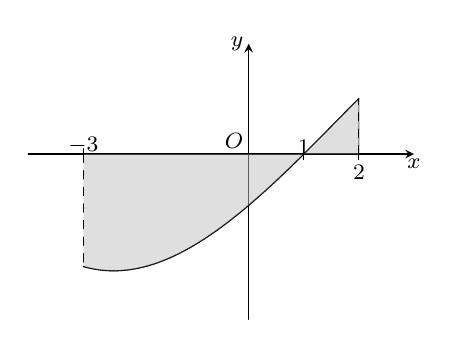
\begin{tikzpicture}[scale=.7,>=stealth,line cap=round,line join=round,font=\footnotesize]
				 \def\a{-0.02}
				 \def\b{0.1}
				 \def\c{0.85}
				 \def\d{-0.93}
				\def\f (#1){\a*((#1)^3)+\b*((#1)^2)+\c*(#1)+\d} 
				 \def\m{-2}
				\def\n{2} 
				 \def\p{8}
				\def\q{0} 
				\def\g (#1){0} 
				 \def\xmin{-4}
				 \def\xmax{3}
				 \def\ymin{-3}
				\def\ymax{2} 
				\draw[->] (\xmin,0)--(\xmax,0) node[below] {$x$}; 
				\draw[->] (0,\ymin)--(0,\ymax)  node[left] {$y$};
				\draw (0,0) node [above left]  {$O$};
				 \clip (\xmin,\ymin) rectangle (\xmax,\ymax);
				\foreach \x in {-3,1}\draw (\x,0.1)--(\x,-0.1) node  [above] {$\x$};
				\foreach  \x in {2}\draw (\x,0.1)--(\x,-0.1) node [below] {$\x$};
				\draw[smooth,samples=200] plot[domain=-3:2] (\x,{\f (\x)}); 
				\draw[fill=gray!50!white,opacity=0.5]  plot[domain=-3:2] (\x,{\g (\x)})--plot[domain=2:-3](\x,{\f (\x)});
				\draw[dashed]  (-3,0)--(-3,-2)
					(2,0)--(2,1); 
			\end{tikzpicture}
	\end{center}
	Mệnh đề nào sau đây đúng? 
	 \choice
		 {$S = -a - b$}
		{$S = a + b$} 
		{$S = a  - b$}
		{\True  $S = b - a$}
	\loigiai{ 
		Ta có: $S =  \displaystyle\int_{-3}^{2} |f(x)| \mathrm{\,d}x = -\displaystyle\int_{-3}^{1} f(x) \mathrm{\,d}x + \displaystyle\int_{1}^{2} f(x) \mathrm{\,d}x = -a + b$.
	 }
\end{ex}

% nguồn: Phan1_Lop_12_Dai_so_Chuong_4
\begin{ex}%[2D4H3-1]%[ma:93eccbb9]
	\immini[thm]{ 
	Tính diện tích phần hình phẳng (phần  gạch chéo) trong hình vẽ bên.
	 \choice
		{\True  $\dfrac{5}{12}$}
		{$\dfrac{9}{4}$} 
		 {$\dfrac{81}{12}$}
		 {$13$}
		} 
		 {
		\begin{tikzpicture}[scale=1.3,font=\footnotesize,line join=round,line cap=round,>=stealth]
				\draw[->] (-1.7,0)--(0,0) node[below left]{$O$}  circle (1pt)--(2,0) node[below]{$x$};
				\draw[->] (0,-1.4)--(0,0)--(0,1.5)  node[right]{$y$};
				\draw [domain=-0.8:1.8,samples=100] plot  (\x,{-1*(\x)^2+(\x)});
				\draw [domain=-1.4:1.4,samples=100] plot (\x,{(\x)^3-(\x)}); 
				\draw[fill]  (1,0) node[below]{$1$} circle (1pt);
				\fill[pattern=north east lines](0,1)  plot[domain=0:1] (\x,{-1*(\x)^2+(\x)})
					(1,1) plot[domain=1:0](\x,{(\x)^3-(\x)}); 
			\end{tikzpicture}
		} 
	 \loigiai{
		Quan sát đồ thị ta thấy phần  diện tích hình phẳng phải tính được giới hạn bởi đồ thị $2$ hàm số $y=x^3-x$, $y=x-x^2$ và $2$ đường thẳng $x=0$, $x=1$.\\
		Đồ thị hàm số $y=x-x^2$ nằm trên đồ thị  hàm số $y=x^3-x$ nên
		 $$S=\displaystyle\int_0^1 \left[x-x^2-(x^3-x)\right]\mathrm{\,d}x=\left(-\dfrac{x^4}{4}-\dfrac{x^3}{3}+x^2\right)\Bigg|_0^1=\dfrac{5}{12}.$$
	 }
\end{ex}

% nguồn: Phan1_Lop_12_Dai_so_Chuong_4
\begin{ex}%[2D4H3-1]%[ma:3aa6a097]
	\immini[thm]{Diện tích  hình phẳng gạch sọc trong hình vẽ bằng
	\choice 
		{$\displaystyle\int_{1}^{3}  2^{x} \mathrm{\, d}x$}
		{$\displaystyle\int_{1}^{3} (2+2^{x}) \mathrm{\, d}x$} 
		 {\True $\displaystyle\int_{1}^{3} |2-2^{x}| \mathrm{\, d}x$}
		{$\displaystyle\int_{1}^{3} 2^{x} dz$}}{\begin{tikzpicture}[>=stealth,line width = 1pt,scale=.6]
		\draw[->]  (-3,0)--(5,0) node[above]{$x$};
		 \draw[->](0,-1) -- (0,9) node[right]{$y$};
		\draw  (0,0) circle (1pt) node[below left]{$O$};
		\clip (-3,-1) rectangle (5,10); 
		\draw[smooth,samples=100,domain=-3:3.2] 
			 plot (\x,{2^(\x)});
		 \draw[smooth,samples=100,domain=1:3]
			 plot (\x,2);
		\draw[pattern = north east lines,line width  = 1pt] (1,2.5)
			plot[domain=1:3] (\x,{2^(\x)})-- plot[domain=3:1]  (\x,2)--cycle;
		\draw (1,0)--  (1,2);
		\draw  (3,0)-- (3,8);
		\draw[dashed](1,2)-- (0,2) node[left]{$2$}; 
		 \draw[dashed](3,8)-- (0,8) node[left]{$8$};
		\begin{scriptsize}
			\draw (1,-0.4) node  {\normalsize $1$};
			 \draw (3,-0.4) node {\normalsize $3$};
			\draw (-1.5,0.8) node  {\normalsize $y=2^x$};
		\end{scriptsize}
	\end{tikzpicture}
		 }
	\loigiai{Hình phẳng đã  cho được giới hạn bởi các đường $$y=2^x,\;y=2,\;x=1,\;x=3.$$
	Vậy diện tích  của hình phẳng là $\displaystyle\int_{1}^{3} |2-2^{x}| \mathrm{\, d}x$.}
\end{ex}

% nguồn: Phan1_Lop_12_Dai_so_Chuong_4
\begin{ex}%[2D4H3-1]%[ma:881ec069]
	 Diện tích của phần hình phẳng gạch chéo trong hình bên bằng
	\begin{center}
		\begin{tikzpicture}[scale=.7,>=stealth,line cap=round,line join=round,font=\footnotesize]
				\def\a{-1} 
				 \def\b{2}
				\def\f  (#1){\a*(#1)^3+\b*(#1)}
				 \def\m{1}
				\def\g (#1){\m*(#1)^2} 
				\def\xmin{-4} 
				 \def\xmax{4}
				\def\ymin{-2} 
				 \def\ymax{4}
				\clip  (\xmin,\ymin) rectangle (\xmax+1.3,\ymax+1.3);
				\draw[->]  (\xmin-1,0)--(\xmax+1,0) node[below] {$x$};
				\draw[->] (0,\ymin-1)--(0,\ymax+1)  node[left] {$y$};
				\draw (0,0) node  [below right] {$O$};
				\draw[smooth,samples=200]  plot[domain=\xmin:\xmax] (\x,{\f (\x)});
				\draw[smooth,samples=200] plot[domain=\xmin:\xmax]  (\x,{\g (\x)});
				\draw[pattern=north west lines,opacity=0.5]  plot[domain=-2:1] (\x,{\f (\x)})--plot[domain=1:-2](\x,{\g (\x)});
				\draw  (.3,4) node[right]{$y=x^2$}
					(2,-1.5)  node[right]{$y=-x^3+2x$};
			\end{tikzpicture}
	\end{center}
	 \choice
		{$\dfrac{55}{12}$} 
		 {\True $\dfrac{37}{12}$}
		{$\dfrac{9}{4}$} 
		 {$\dfrac{15}{4}$}
	 \loigiai{
		Giải phương trình $x^2 = -x^3 + 2x \Leftrightarrow x^3 + x^2 - 2x = 0 \Leftrightarrow \begin{cases} x = 1 \\ x = 0 \\ x = -2
	\end{cases}$.\\
	Diện tích của phần hình phẳng gạch chéo trong hình bên $S =  \displaystyle\int_{-2}^{1} |x^3 + x^2 - 2x| \mathrm{\,d}x = \dfrac{37}{12}$.
 }
\end{ex}

% nguồn: Phan1_Lop_12_Dai_so_Chuong_4
\begin{ex}%[2D4H3-1]%[ma:6a2795dc]
	Tính diện tích hình phẳng  giới hạn bởi đồ thị hàm số $y = x^3 - x$ và $y = x - x^2$.
	 \choice
		 {$13$}
		{$V =  \dfrac{81}{12}$}
		{$\dfrac{9}{4}$} 
		{\True $\dfrac{37}{12}$} 
	\loigiai{ 
		Phương trình hoành độ  giao điểm đồ thị hàm số $y = x^3 - x$ và $y = x - x^2$ là $x^3 - x = x - x^2$.\\
		Ta có $ x^3 + x^2 - 2x = 0 \Leftrightarrow \begin{cases} x = 0 \\ x = 1 \\ x = -2.
	\end{cases}$\\
	Suy ra 
	\begin{eqnarray*}
		S&= & \displaystyle\int_{-2}^{1} |x^3 + x^2  - 2x| \mathrm{\,d}x\\
		&= & \displaystyle\int_{-2}^{0} (x^3 + x^2 -  2x) \mathrm{\,d}x - \displaystyle\int_{0}^{1} (x^3 + x^2 - 2x) \mathrm{\,d}x\\
		&= & \left( \dfrac{x^4}{4} + \dfrac{x^3}{3} - x^2 \right) \Big|_{-2}^{0} - \left( \dfrac{x^4}{4} + \dfrac{x^3}{3} - x^2  \right) \Big|_{0}^{1}=0\\
		 & =&\dfrac{8}{3} - \left( -\dfrac{5}{12} \right) = \dfrac{37}{12}.
	\end{eqnarray*}
 }
\end{ex}

% nguồn: Phan1_Lop_12_Dai_so_Chuong_4
\begin{ex}%[2D4H3-1]%[ma:c921bc31]
	Diện tích hình  phẳng giới hạn bởi đồ thị các hàm số $y=x^3-3x$ và $y=x$ bằng
	 \choice
		 {$ 0$}
		 {\True $ 8$}
		 {$ 2$}
		{$  4$}
	\loigiai{ 
		Xét  phương trình $x^3-3x=x\Leftrightarrow x^3-4x=0\Leftrightarrow
		\hoac{& x=0\\ 
		&  x=\pm 2.}$\\
		 Diện tích hình phẳng giới hạn bởi đồ thị các hàm số $y=x^3-3x$ và $y=x$ là
		\begin{align*}
			 S&=\displaystyle\int_{-2}^2\left|x^3-4x\right|\mathrm{\,d}x=\displaystyle\int_{-2}^0\left|x^3-4x\right|\mathrm{\,d}x+\displaystyle\int_0^2\left|x^3-4x\right|\mathrm{\,d}x\\
			&=\left|\left.\left(\dfrac{x^4}{4}-2x^2\right)\right|^0_{-2}\right| 
			 +\left|\left.\left(\dfrac{x^4}{4}-2x^2\right)\right|_0^2\right|=8.
	\end{align*}}
\end{ex}

% nguồn: Phan1_Lop_12_Dai_so_Chuong_4
\begin{ex}%[2D4H3-1]%[ma:94bf5110]
	Tính diện tích hình phẳng  giới hạn bởi đồ thị hàm số $ y=x^2+2x+1$, trục hoành và hai đường thẳng $ x=-1$; $x=3$.
	\choice 
		{$ S=\dfrac{37}{3}$} 
		{$  S=\dfrac{56}{3}$}
		{$  S=\dfrac{68}{3}$}
		{\True $ S=\dfrac{64}{3}$} 
	 \loigiai{
		Diện tích hình phẳng giới hạn bởi đồ thị hàm số $ y=x^2+2x+1$, trục hoành và hai đường thẳng $ x=-1$; $x=3$ là \begin{center}
		 $S=\displaystyle\int_{-1}^3\left|x^2+2x+1\right|\mathrm{\,d}x=\displaystyle\int_{-1}^3\left(x^2+2x+1\right)\mathrm{\,d}x=\left.\left(\dfrac{x^3}{3}+x^2+x\right)\right|^3_{-1}=\dfrac{64}{3}$.
\end{center}}
\end{ex}

% nguồn: Phan1_Lop_12_Dai_so_Chuong_4
\begin{ex}%[2D4H3-1]%[ma:fb63554c]
	Diện tích của hình phẳng giới hạn  bởi các đường thẳng $y = e^{\frac{x}{2}}$, $y = 0$ và $x = 0$; $x = 2$ bằng
	\choice 
		 {\True $2e - 2$}
		{$\dfrac{e - 1}{2}$} 
		{$2e$} 
		{$e - 1$} 
	 \loigiai{
		Diện tích hình phẳng giới hạn bởi các đường  thẳng $y = e^{\frac{x}{2}}$, $y = 0$ và $x = 0; x = 2$ là:
		$S = \displaystyle\int_{0}^{2} |e^{\frac{x}{2}}| \mathrm{\,d}x = \displaystyle\int_{0}^{2} e^{\frac{x}{2}} \mathrm{\,d}x = \left. 2e^{\frac{x}{2}} \right|_{0}^{2} = 2(e^{\frac{2}{2}} - e^{\frac{0}{2}}) = 2(e - 1) = 2e - 2$. 
	} 
\end{ex}

% nguồn: Phan1_Lop_12_Dai_so_Chuong_4
\begin{ex}%[2D4H3-1]%[ma:9da030cb]
	Diện tích hình phẳng giới hạn bởi parabol  $(P)\colon y=-x^{2}+4$ và trục hoành bằng
	 \choice
		{$\dfrac{16}{3}$} 
		{$-\dfrac{32}{3}$} 
		{\True $\dfrac{32}{3}$} 
		{$\dfrac{20  \sqrt{2}}{3}$}
	\loigiai{ 
		Phương trình hoành độ  giao điểm của $(P)$ và $Ox$ là $-x^{2}+4=0\Leftrightarrow\hoac{& x=-2\\& x=2.}$\\
		Diện tích hình  phẳng cần tìm là $S=\displaystyle\int_{-2}^{2} |-x^2+4| \mathrm{\,d}x=\left[-\frac{x^3}{3} + 4x\right]\Bigg| _{-2}^{2} = \frac{32}{3}$.
	} 
\end{ex}

% nguồn: Phan1_Lop_12_Dai_so_Chuong_4
\begin{ex}%[2D4H3-1]%[ma:1de23044]
	Diện tích hình phẳng gạch sọc trong hình vẽ bên dưới  bằng
	\begin{center}
		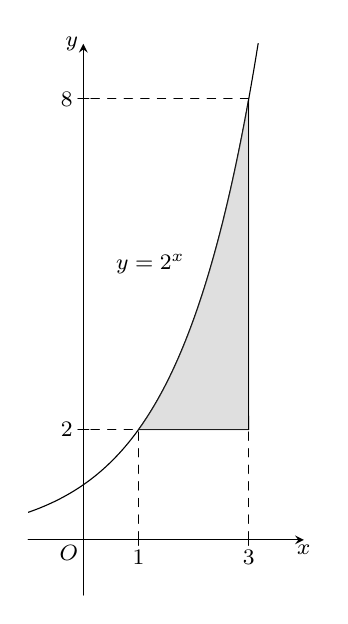
\begin{tikzpicture}[scale=.7,>=stealth,line cap=round,line join=round,font=\footnotesize]
				 \def\a{2}
				 \def\b{-3}
				 \def\c{2}
				 \def\d{0}
				 \def\f (#1){\a^(#1)}
				 \def\m{-2}
				\def\n{2} 
				\def\p{8} 
				\def\q{0} 
				\def\g (#1){2} 
				\def\xmin{-1} 
				 \def\xmax{4}
				 \def\ymin{-1}
				 \def\ymax{9}
				\draw[->]  (\xmin,0)--(\xmax,0) node[below] {$x$};
				\draw[->] (0,\ymin)--(0,\ymax) node[left]  {$y$};
				 \draw (0,0) node [below left] {$O$};
				\clip  (\xmin,\ymin) rectangle (\xmax,\ymax);
				 \foreach \x in {1,3}\draw (\x,0.1)--(\x,-0.1) node [below] {$\x$};
				\foreach \y in {2,8}\draw (0.1,\y)--(-0.1,\y)  node [left] {$\y$};
				\draw[smooth,samples=200] plot[domain=\xmin:\xmax]  (\x,{\f (\x)});
				\draw[smooth,samples=200] plot[domain=1:3] (\x,{\g  (\x)});
				 \draw[fill=gray!50!white,opacity=0.5] plot[domain=1:3] (\x,{\f (\x)})--plot[domain=3:1](\x,{\g (\x)});
				\draw (.5,5) node[right]{$y=2^x$}; 
				 \draw[dashed] (1,0)--(1,2)--(0,2)
					 (3,0)--(3,2)
					 (3,8)--(0,8);
				 \draw (3,2)--(3,8);
			\end{tikzpicture}
	\end{center}
	 \choice
		{\True $\displaystyle\int_{1}^{3} (2^x - 2) \mathrm{\,d}x$} 
		{$\displaystyle\int_{1}^{3}  (2^x + 2) \mathrm{\,d}x$}
		{$\displaystyle\int_{1}^{3}  (2 - 2^x) \mathrm{\,d}x$}
		{$\displaystyle\int_{1}^{3}  2^x \mathrm{\,d}x$}
	\loigiai{ 
		Hình phẳng gạch sọc  trong hình vẽ được giới hạn bởi các đường $y = 2^x$, $y = 2$, $x = 1$ và $x = 3$.\\
		Do đó diện tích hình phẳng gạch sọc trong hình vẽ bằng $\displaystyle\int_{1}^{3} |2^x - 2| \mathrm{\,d}x = \displaystyle\int_{1}^{3} (2^x  - 2) \mathrm{\,d}x$.
	} 
\end{ex}

% nguồn: Phan1_Lop_12_Dai_so_Chuong_4
\begin{ex}%[2D4H3-1]%[ma:cfea2200]
	Cho hàm số $y=f(x)$ liên tục trên $\mathbb{\mathrm{R}}$ và có đồ thị cắt trục $Ox$ tại đúng ba điểm phân biệt $a$, $b$, $c$ $(a<c<b)$. Gọi $S_1$ là diện tích hình phẳng giới hạn bởi đồ thị hàm số và trục ${Ox}$ tương ứng với $x\in \left[a;c \right]$, $S_2$ là  diện tích hình phẳng giới hạn bởi đồ thị hàm số và trục ${Ox}$ tương ứng với $x \in \left[c;b \right]$. Nếu $f(x)\ge 0,\,\forall x\in \left[a;c \right],f(x)\ge 0,\,\forall x\in \left[c;b \right]$ thì giá trị của $\displaystyle\int_a^b f(x)\mathrm{\,d}x$ bằng
	\choice 
		{\True  $S_1+S_2$}
		{$S_1-S_2$} 
		 {$- S_1+ S_2$}
		{$- S_1- S_2$} 
	\loigiai{ 
		$\displaystyle\int_a^b f(x)\mathrm{\,d}x =  S_1+S_2$.
	} 
\end{ex}

% nguồn: Phan1_Lop_12_Dai_so_Chuong_4
\begin{ex}%[2D4H3-1]%[ma:c878cc06]
	Diện tích $S$  hình phẳng $(H)$ giới hạn bởi đường cong $y=-x^3+12x$ và $y=-x^2$ bằng
	 \choice
		 {\True $S=\dfrac{937}{12}$}
		 {$S=\dfrac{343}{12}$}
		{$S=\dfrac{397}{4}$} 
		 {$S=\dfrac{793}{4}$}
	 \loigiai{
		Xét phương trình  $-x^3+12x=-x^2\Leftrightarrow
		 \hoac{
		&  x=0\\
		&  x=4\\
		&  x=-3.}$\\
		Diện tích $S$ hình phẳng $(H)$ giới hạn  bởi đường cong $y=-x^3+12x$ và $y=-x^2$ bằng
		\begin{center}
			 $S=\displaystyle\int_{-3}^4\left|-x^3+12x+x^2\right|\mathrm{\,d}x=\dfrac{937}{12}$.
		\end{center}
	 }
\end{ex}

% nguồn: Phan1_Lop_12_Dai_so_Chuong_4
\begin{ex}%[2D4H3-1]%[ma:0786166f]
	 Cho hàm số $y=f(x)$ liên tục trên $\mathrm{R}$ và có đồ thị cắt trục $Ox$ tại đúng hai điểm phân biệt $a$, $b$. Gọi S là diện tích hình phẳng giới hạn bởi đồ thị hàm số $y=f(x)$ và trục $Ox$. Nếu $f(x)\le 0$, $\forall x\in \left[a;b \right]$ thì
	\choice 
		{$\displaystyle\int_a^b  f(x)\mathrm{\,d}x =S$}
		{$\displaystyle\int_a^b f(x)\mathrm{\,d}x  =(a-b)S$}
		{\True  $\displaystyle\int_a^b f(x)\mathrm{\,d}x =-S$}
		{$\displaystyle\int_a^b f(x)\mathrm{\,d}x  =(b-a)S$}
	 \loigiai{
		$\displaystyle\int_a^b f(x)\mathrm{\,d}x =-S$. 
	} 
\end{ex}

% nguồn: Phan1_Lop_12_Dai_so_Chuong_4
\begin{ex}%[2D4H3-1]%[ma:159c6998]
	Diện tích hình phẳng giới hạn bởi các đường $y =  x^2$ và $y = 4x - 3$ là
	 \choice
		 {$S = \dfrac{3}{4}$}
		 {\True $S = \dfrac{4}{3}$}
		{$S = \dfrac{2}{3}$} 
		{$S  = 2$}
	\loigiai{ 
		Phương trình hoành độ giao điểm $x^2 = 4x - 3 \Leftrightarrow x^2 - 4x + 3 = 0 \Leftrightarrow \begin{cases} x = 1 \\ x = 3
	\end{cases}$.\\
	Khi đó $S = \left| \displaystyle\int_{1}^{3}  x^2 - 4x + 3 \mathrm{\,d}x \right| = \dfrac{4}{3}$.
} 
\end{ex}

% nguồn: Phan1_Lop_12_Dai_so_Chuong_4
\begin{ex}%[2D4H3-1]%[ma:9669e054]
	Diện tích hình phẳng giới hạn bởi $ 2$ đường $ y=x^2-1$ và $  y=x-1$ bằng
	 \choice
		 {$\dfrac{\pi}{6}$}
		 {$\dfrac{13}{6}$}
		{$\dfrac{13\pi}{6}$} 
		 {\True $\dfrac{1}{6}$}
	\loigiai{ 
		Phương trình hoành độ giao điểm  hai đồ thị hàm số là $x^2-1=x-1\Leftrightarrow x^2-x=0\Leftrightarrow
		 \hoac{& x=0\\
		&  x=1.}$\\
	Diện  tích hình phẳng là $S=\displaystyle\int_0^1\left|x^2-x\right|\mathrm{\,d}x=\left|\displaystyle\int_0^1\left(x^2-x\right)\mathrm{\,d}x\right|=\left|\left.\left(\dfrac{x^3}{3}-\dfrac{x^2}{2}\right)\right|_0^1\right|=\dfrac{1}{6}$.}
\end{ex}

% nguồn: Phan1_Lop_12_Dai_so_Chuong_4
\begin{ex}%[2D4H3-1]%[ma:b23e3377]
	\immini{Công thức nào sau đây mô tả diện tích của  phần gạch chéo trong hình vẽ bên?
	 \choice
		{$S=\displaystyle  \int_{-1}^{2} \left(2x^2-2x-4\right)\mathrm{\,d}x$}
		{\True$S=\displaystyle \int_{-1}^{2}  \left(-2x^2+2x+4\right)\mathrm{\,d}x$}
		 {$S=\displaystyle \int_{-1}^{2} \left(-2x+2\right)\mathrm{\,d}x$}
		{$S=\pi \displaystyle \int_{-1}^{2} \left(2x^2+2x-4\right)\mathrm{\,d}x$}}{	\begin{tikzpicture}[x=0.7cm,y=0.7cm,>=stealth,font=\footnotesize]
		 \def\xmin{-1.23};
		\def\xmax{3.23}; 
		 \def\ymin{-2};
		\def\ymax{3}; 
		\draw[->,color=black]  (\xmin-0.3,0) -- (\xmax+1,0) node[below] {$x$};
		\draw[->,color=black] (0,\ymin) -- (0,\ymax+0.8) node[right]{$y$}; 
		\draw (0,0) node[below  right] {$O$};
		\draw[smooth] plot[domain=\xmin-0.3:\xmax-1](\x,{-(\x)^2+3})  node[right]{$y=-x^2+3$};
		\draw[smooth] plot[domain=-1.4:3.4](\x,{(\x)^2-2*(\x)-1})  node[right]{$y=x^2-2x-1$};
		\draw[dashed,smooth]  (-1,2)--(-1,0)
			(2,-1)--(2,0); 
		\foreach  \x in {-1}
		\draw[shift={(\x,0)},color=black] (0pt,2pt) -- (0pt,-2pt)  node[below]{$\x$};
		\foreach \x in {2} 
		\draw[shift={(\x,0)},color=black] (0pt,2pt) -- (0pt,-2pt)  node[above]{$\x$};
		\fill[pattern=north east lines,smooth] (-1,2) --plot[domain=-1:2](\x,{-(\x)^2+3})--plot[domain=2:-1](\x,{(\x)^2-2*(\x)-1})--(-1,2)-- cycle; 
	\end{tikzpicture}
		 }
	\loigiai{Dựa vào  đồ thị, ta có $-x^2+3 \ge x^2-2x-1$,$\forall x \in [-1;2]$.\\
		Do đó $(-x^2+3)-( x^2-2x-1) \ge  0$,$\forall x \in [-1;2]$ hay $-2x^2+2x+4 \ge 0$,$\forall x \in [-1;2]$.\\
	Diện tích phần gạch chéo là diện tích phần hình phẳng được giới hạn bởi đồ thị của hàm số $y=-x^3+3$, $y=x^2-2x-1$ và hai đường thẳng $x=-1$,  $x=2$. Do đó $$S=\displaystyle \int_{-1}^{2} \left|(-x^2+3)-( x^2-2x-1)\right|\mathrm{\,d}x=\displaystyle \int_{-1}^{2} \left|-2x^2+2x-4\right|\mathrm{\,d}x=\displaystyle \int_{-1}^{2} \left(-2x^2+2x+4\right)\mathrm{\,d}x.$$}
\end{ex}

% nguồn: Phan1_Lop_12_Dai_so_Chuong_4
\begin{ex}%[2D4H3-1]%[ma:caafb31b]
	\immini[thm]{Cho hàm số $ y=f(x)$ liên tục trên $\mathbb{R}$ và có đồ thị $(C)$ là đường cong như hình bên. Diện tích hình phẳng giới hạn bởi  đồ thị hàm số $(C)$, trục hoành và hai đường thẳng $ x=0$; $ x=2$ là
	\choice 
		{\True  $\displaystyle\int_0^1f(x)\mathrm{\,d}x-\displaystyle\int_1^2f(x)\mathrm{\,d}x$}
		 {$\displaystyle\int_0^1f(x)\mathrm{\,d}x+\displaystyle\int_1^2f(x)\mathrm{\,d}x$}
		{$\left|\displaystyle\int_0^2f(x)\mathrm{\,d}x\right|$} 
		{$\displaystyle\int_0^2f(x)\mathrm{\,d}x$} 
		}{\begin{tikzpicture}[line join=round,line cap=round,>=stealth,scale=0.85,font=\footnotesize]
		\tikzset{every node/.style={outer  sep=-0.5mm}}
		\def \xmin{-3}  \def \xmax{3.5}
		 \def \ymin{-2} \def \ymax{4}
		 \def \fx{(\x+2)^2*(\x-1)*(\x-2.5)/5}
		 \draw[->] (\xmin,0)--(\xmax,0) node[below left] {\normalsize$x$};
		\draw[->] (0,\ymin)--(0,\ymax) node[below left]  {\normalsize$y$};
		\fill  (0,0) circle (1.25pt) node[below left] {$O$};
		\fill (1,0) circle (1.25pt) node[below,xshift=-1mm] {$1$}; 
		\fill (2,0) circle  (1.25pt) node[above] {$2$};
		\begin{scope}
			 \clip (\xmin+0.01,\ymin+0.01) rectangle (\xmax-0.01,\ymax-0.01);
			\draw[samples=150,domain=\xmin+0.01:2.9,smooth,variable=\x]  plot (\x,{\fx}) node[left]{$y=f (x)$};
			\draw[pattern=north east lines,opacity=0.5] (0,0)--plot[domain=0:2]  (\x,{\fx})--(2,0)--cycle;
		\end{scope}
	\end{tikzpicture}}
	 \loigiai{
	Dựa vào đồ thị hàm số ta có diện tích hình  phẳng cần tính là $\displaystyle\int_0^1f(x)\mathrm{\,d}x-\displaystyle\int_1^2f(x)\mathrm{\,d}x$.}
\end{ex}

% nguồn: Phan1_Lop_12_Dai_so_Chuong_4
\begin{ex}%[2D4H3-1]%[ma:08c8eaac]
	Diện tích của hình phẳng giới hạn bởi đồ thị của  hai hàm số $y=x^3, y=x$ và hai đường thẳng $x=0, x=2$ bằng
	\choice 
		{$2$} 
		{\True $\dfrac{5}{2}$} 
		 {$\dfrac{9}{4}$}
		{$\dfrac{1}{4}$} 
	 \loigiai{
		Diện tích cần tìm là $S=\displaystyle\int_{0}^{2}  |x^3-x|\mathrm{\,d}x$.\\
		Ta có $x^3-x=0 \Leftrightarrow  x=0$ hoặc $x=1$ hoặc $x=-1$ .\\
		Phương trình chỉ có hai nghiệm thuộc đoạn  $[0;2]$ là $x=0$ và $x=1$.
		\begin{align*}
			\text{ Vậy } S&=\displaystyle\int_{0}^{2} |x^3-x|\mathrm{\,d}x=\displaystyle\int_{0}^{1}  |x^3-x|\mathrm{\,d}x+\displaystyle\int_{1}^{2} |x^3-x|\mathrm{\,d}x\\
			&=\left|\displaystyle\int_{0}^{1}  (x^3-x)\mathrm{\,d}x\right|+\left|\displaystyle\int_{1}^{2} (x^3-x)\mathrm{\,d}x\right|\\
			&=\left|\left(\dfrac{x^4}{4}-\dfrac{x^2}{2}\right)\bigg|_{0}^{1}\right|+\left|\left(\dfrac{x^4}{4}-\dfrac{x^2}{2}\right)\bigg|_{1}^{2}\right|=\left|-\dfrac{1}{4}\right|+\left|\dfrac{9}{4}\right|=\dfrac{5}{2}. 
		\end{align*}
	 }
\end{ex}

% nguồn: Phan1_Lop_12_Dai_so_Chuong_4
\begin{ex}%[2D4H3-1]%[ma:7669b35f]
	Diện tích hình phẳng giới hạn bởi đồ thị hàm số $y = x^2 + 2$ và đường  thẳng $y = 6$ bằng
	\choice 
		{\True $\dfrac{32}{3}$} 
		 {$\dfrac{40}{3}$}
		 {$\dfrac{16}{3}$}
		 {$\dfrac{8}{3}$}
	\loigiai{ 
		Phương trình hoành độ giao điểm $x^2 + 2  = 6 \Leftrightarrow x^2 = 4 \Leftrightarrow x = \pm 2$.\\
		Diện tích hình  phẳng cần tìm là $S = \displaystyle\int_{-2}^{2} |x^2 - 4| \mathrm{\,d}x = \dfrac{32}{3}$
	 }
\end{ex}

% nguồn: Phan1_Lop_12_Dai_so_Chuong_4
\begin{ex}%[2D4H3-1]%[ma:45bbd376]
	Biết $F(x)$ và $G(x)$ là hai nguyên hàm của hàm số  $f(x)$ trên $\mathbb{R}$ và thoả mãn
	$\displaystyle\int_{0}^{4} f(x) \mathrm{\,d}x  = F(4) - G(0) + 2m$, với $m > 0$. Gọi $S$ là diện tích hình phẳng giới hạn bởi các đường
	$y = F(x)$, $y  = G(x)$; $x = 0$ và $x = 4$. Khi $S = 8$ thì $m$ bằng
	\choice 
		{\True  $1$}
		{$2$} 
		 {$3$}
		{$4$} 
	 \loigiai{
		Theo đề ta có 
		\begin{eqnarray*}
			&  & \displaystyle\int_{0}^{4} f(x) \mathrm{\,d}x = F(4) - G(0) + 2m\\
			&\Leftrightarrow  & F(x) \Big|_{0}^{4} = F(4) - G(0) + 2m\\
			&\Leftrightarrow & F(4) - F(0) = F(4) - G(0)  + 2m\\
			&\Leftrightarrow & G(0) - F(0) = 2m.  (1)
		\end{eqnarray*}
		Mặt khác, do $F(x)$ và  $G(x)$ là hai nguyên hàm của hàm số $f(x)$ trên $\mathbb{R}$ nên ta có $G(x) - F(x) = C$ (không đổi với mọi $x \in \mathbb{R}$). $(2)$\\
		Từ $(1)$ và $(2)$ suy ra $G(x) - F(x) = 2m >  0$, với mọi $x \in \mathbb{R}$.\\
		Khi đó ta có $S = \displaystyle\int_{0}^{4} |G(x) - F(x)| \mathrm{\,d}x = \displaystyle\int_{0}^{4} 2m \mathrm{\,d}x  = 2m x \Big|_{0}^{4} = 8m$.\\
		Theo đề  ta có $8m = 8 \Leftrightarrow m = 1$.
	 }
\end{ex}

% nguồn: Phan1_Lop_12_Dai_so_Chuong_4
\begin{ex}%[2D4H3-1]%[ma:0a93cff9]
	Diện tích hình thang cong giới hạn bởi $y=\dfrac2{x+1}$; $y=0$;  $x=1$; $x=3$ bằng
	\choice 
		{$S=\ln  8$}
		 {\True $S=\ln 4$}
		{$S=2\ln  4$}
		{$S=\ln  2$}
	\loigiai{ 
		Ta  có\\
		$ f(x)=\dfrac2{x+1}$ là hàm số liên tục  và không âm trên đoạn $[1;3]$.\\
		$F(x)=2\ln|x+1 |$ là một nguyên hàm  của hàm số $ f(x)=\dfrac2{x+1}$ trên $\left[1;3\right]$.\\
		Do đó diện tích hình thang cong  cần tìm là
		\[S=F(3)-F(1)=2\ln 4-2\ln 2=2\ln 2=\ln 4.\] 
	 }
\end{ex}

% nguồn: Phan1_Lop_12_Dai_so_Chuong_4
\begin{ex}%[2D4H3-1]%[ma:e330c76c]
	Diện tích hình phẳng giới hạn bởi đồ thị hàm số $y=x^2$ và  đường thẳng $y=2x$ là
	\choice 
		{\True $\dfrac{4}{3}$} 
		{$\dfrac{5}{3}$} 
		 {$\dfrac{3}{2}$}
		{$\dfrac{23}{15}$} 
	 \loigiai{
		Xét phương trình  $x^2=x \Rightarrow\hoac{&x=0\\&x=1.}$\\
		Diện tích hình phẳng giới hạn bởi đồ thị hàm số  $y=x^2$ và đường thẳng $y=2x$ là
		\begin{align*}
			S=\displaystyle\int_0^1\left|x^2-x\right|\mathrm{\,d}x=\left|\displaystyle\int_0^1\left(x^2-x\right) \mathrm{\,d}x\right|=\dfrac{4}{3}. 
		\end{align*}
	 }
\end{ex}

% nguồn: Phan1_Lop_12_Dai_so_Chuong_4
\begin{ex}%[2D4H3-1]%[ma:2232d996]
	\immini{Hình phẳng giới hạn bởi đồ thị hàm số $y=e^{x}$ và  các đường thẳng $y=1$, $x=-1$ có diện tích là
	 \choice
		{\True  $\dfrac{1}{e}$}
		{$1-\dfrac{1}{e}$} 
		 {$e-1$}
		 {$e$}
		}{ 
		\begin{tikzpicture}[line join=round,line cap=round,>=stealth]
				\draw[->] (-4,0)--(2.5,0) node[below left] {$x$}; 
				\draw[->] (0,-1.5)--(0,3) node[below  left] {$y$};
				\draw (0,0)  node [shift={(-130:3mm)}] {$O$};
				\draw[domain=-4:1.02,smooth,variable=\x] plot ({\x},{exp (\x)}); 
				\draw[domain=-4:2.5,smooth,variable=\x] plot ({\x},1); 
				\draw  (-1,-1.5)--(-1,3);
				\draw (-1,0)  node[shift={(-135:3mm)}] {$-1$};
				\draw (0,1) node[shift={(135:3mm)}] {$1$}; 
			\end{tikzpicture}
		} 
	\loigiai{ 
		Diện tích 
		$S=\displaystyle \int_{-1}^{0} |1-e^x|  \mathrm{\,d}x = \int_{-1}^{0} \left(1-e^x\right) \mathrm{\,d}x = \left(x-e^x\right)\bigg|_{-1}^0 = \dfrac{1}{e}$.
	 }
\end{ex}

% nguồn: Phan1_Lop_12_Dai_so_Chuong_4
\begin{ex}%[2D4H3-1]%[ma:e3d8b918]
	Diện tích hình phẳng giới hạn bởi các đường cong $ y=x^3-6x$ và $ y=x^2$ bằng 
	 \choice
		{$\dfrac{125}{12}$} 
		{$\dfrac{16}{3}$} 
		{$\dfrac{63}{4}$} 
		 {\True $\dfrac{253}{12}$}
	 \loigiai{
		Ta  có $x^3-6x=x^2\Leftrightarrow{x^3}-x^2-6x=0\Leftrightarrow
		 \hoac{
		&  x=3\\
		& x=0\\ 
		&  x=-2.}$\\
	Ta có  $S=\displaystyle\int_{-2}^3\left|x^3-x^2-6x\right|\mathrm{\,d}x=\dfrac{253}{12}$.}
\end{ex}

% nguồn: Phan1_Lop_12_Dai_so_Chuong_4
\begin{ex}%[2D4H3-1]%[ma:1a412aa5]
	Diện tích hình phẳng giới hạn  bởi đồ thị hàm số $y = x^2 + 2x$ và trục hoành bằng
	 \choice
		{$\dfrac{4\pi}{3}$} 
		 {\True $\dfrac{4}{3}$}
		{$\dfrac{3}{4}$} 
		 {$\dfrac{3\pi}{4}$}
	 \loigiai{
		Xét phương trình hoành độ giao điểm: $x^2 + 2x = 0 \Leftrightarrow \begin{cases} x = 0 \\ x = -2.
	\end{cases}$.\\
	Khi đó, diện tích hình phẳng  giới hạn bởi hai đồ thị trên là $S = \displaystyle\int_{-2}^{0} |x^2 + 2x| \mathrm{\,d}x = \dfrac{4}{3}$.
 }
\end{ex}

% nguồn: Phan1_Lop_12_Dai_so_Chuong_4
\begin{ex}%[2D4H3-1]%[ma:8df0c9cb]
	Diện tích hình thang cong giới  hạn bởi $y=x^2$; $y=0$; $x=1$; $x=3$ bằng
	 \choice
		 {$S=6$}
		{\True $S=\dfrac{26}3$} 
		 {$S=5$}
		{$S=\dfrac{28}3$} 
	 \loigiai{
		 Ta có\\
		$ f(x)={x^2}$ là hàm số liên tục và không âm  trên đoạn $[1;3]$.\\
		$F(x)=\dfrac{x^3}3$ là một  nguyên hàm của hàm số $ f(x)={x^2}$ trên $\left[1;3\right]$.\\
		Do đó diện tích hình thang cong cần tìm là \[S=F(3)-F(1)=\dfrac{{3^3}-{1^3}}3=\dfrac{26}3.\] 
	} 
\end{ex}

% nguồn: Phan1_Lop_12_Dai_so_Chuong_4
\begin{ex}%[2D4H3-1]%[ma:910adf2c]
	Hình phẳng giới hạn bởi đồ thị hàm số $y=x^2$ và  đường thẳng $y=2x + 3$ có diện tích là
	 \choice
		 {$\dfrac{49}{3}$}
		 {$\dfrac{29}{3}$}
		{$\dfrac{22}{3}$} 
		 {\True $\dfrac{44}{3}$}
	\loigiai{ 
		Xét $x^2 = 2x +  3 \Leftrightarrow x^2 -2x - 3 = 0 \Leftrightarrow \hoac{&x=-1\\&x=3.}$\\
		Diện  tích
		\begin{align*}
			S &= \displaystyle  \int_{-1}^{3} |x^2-(2x+3)| \mathrm{\,d}x
			=  \displaystyle \int_{-1}^{3} -(x^2-2x-3) \mathrm{\,d}x
			 = \displaystyle \int_{-1}^{3} \left(-x^2+2x+3\right) \mathrm{\,d}x\\
			&=\left(-\dfrac{x^3}{3} +  x^2 + 3x\right)\bigg|_{-1}^3
			 =\dfrac{44}{3}.
		\end{align*}
	 }
\end{ex}

% nguồn: Phan1_Lop_12_Dai_so_Chuong_4
\begin{ex}%[2D4H3-1]%[ma:65fb7740]
	\immini{Cho hàm số $y = f(x)$ liên tục trên $\mathbb{R}$, gọi $(H)$ là hình phẳng giới hạn bởi nửa đường tròn có bán  kính $r = 2$ và đồ thị $(C)$ của hàm số $y = f(x)$ như hình vẽ. Biết $(H)$ có diện tích $S = \dfrac{31}{4}$. Ta có
	\[ 
	 \displaystyle\int_{-2}^{2} f(1 - x)\,\mathrm{d}x = a\pi + \dfrac{b}{2}.
	\] 
	Tính $a + b$.} 
	{\begin{tikzpicture}[scale=1.2]
		\draw[->] (-1.5,0) -- (3.5,0)  node[right] {$x$};
		\draw[->]  (0,-0.5) -- (0,4) node[above] {$y$};
		 \fill[pattern=north east lines,pattern color=black!60,domain=-1:3,variable=\x]
			 (-1,2)
			.. controls (0,1.2) and  (2,1.2)..
			(3,2)  --
			plot[domain=3:-1,samples=100] (\x,{2 + sqrt  (4 - (\x - 1)^2)})
			-- cycle; 
		 \draw
			 plot[domain=-1:3,samples=100]
			(\x,{2 + sqrt (4 - (\x  - 1)^2)})
			node[right] {$(C)\colon y  = f (x)$};
		 \draw
			 (-1,2)
			.. controls (0,1.2) and (2,1.2).. 
			(3,2); 
		\draw[dashed] (-1,0) --  (-1,2);
		\draw[dashed]  (3,0) -- (3,2);
		\draw[dashed]  (-1,2) -- (3,2);
		 \node[below right] at (0,0) {O};
		\node  at (-1,-0.3) {$-1$};
		\node at (3,-0.3)  {$3$};
		 \node[above left] at (0,2) {$2$};
	\end{tikzpicture}
	 }
	\choice 
		{$a + b =  \dfrac{3}{2}$}
		{\True  $a + b = \dfrac{5}{2}$}
		{$a  + b = 3$}
		 {$a + b = -\dfrac{5}{2}$}
	 \loigiai{
		Đặt $I = \displaystyle\int_{-2}^{2} f(1 - x)\,\mathrm{d}x$. Đặt $u = 1 - x \Rightarrow \mathrm{d}u = -\mathrm{d}x$. Khi $x = -2 \Rightarrow u = 3$, $x = 2 \Rightarrow u = -1$. Ta  có
		\[ 
		I = \displaystyle\int_{-2}^{2} f(1 - x)\,\mathrm{d}x =  - \displaystyle\int_{3}^{-1} f(u)\,\mathrm{d}u = \displaystyle\int_{-1}^{3} f(x)\,\mathrm{d}x.
		\] 
		Từ hình vẽ và giả thiết,  ta có
		\begin{eqnarray*}
			&S&=\left(2\cdot  4-\displaystyle\int_{-1}^3f(x)\,\mathrm{d}x\right)+2\pi\\
			&\Leftrightarrow&\dfrac{31}{4}=8-a\pi-\dfrac{b}{2}+2\pi\\ 
			&\Leftrightarrow&(2-a)\pi+\left(\dfrac{1}{4}-\dfrac{b}{2}\right)=0\\ 
			 &\Rightarrow&a=2; b=\dfrac{1}{2}.
		\end{eqnarray*}
		Vậy $a +  b = \dfrac{5}{2}$.
	} 
\end{ex}

% nguồn: Phan1_Lop_12_Dai_so_Chuong_4
\begin{ex}%[2D4H3-1]%[ma:9c3dd1df]
	Diện tích hình phẳng $S$ giới hạn bởi các đường thẳng $ y=x^2-x$, $y=0$, $x=0$, $x=2$ được  tính bởi công thức nào sau đây?
	\choice 
		{$ S=\displaystyle\int_0^2\left(x-x^2\right)\mathrm{\,d}x$} 
		{\True  $S=\displaystyle\int_1^2\left(x^2-x\right)-\displaystyle\int_0^1\left(x^2-x\right)\mathrm{\,d}x$}
		{$ S=\displaystyle\int_0^1\left(x^2-x\right)+\displaystyle\int_1^2\left(x^2-x\right)\mathrm{\,d}x$} 
		{$  S=\displaystyle\int_0^2\left(x^2-x\right)\mathrm{\,d}x$}
	\loigiai{ 
	Ta có $  S=\displaystyle\int_0^2\left|x^2-x\right|\mathrm{\,d}x=\displaystyle\int_0^1\left|x^2-x\right|\mathrm{\,d}x+\displaystyle\int_1^2\left|x^2-x\right|\mathrm{\,d}x=-\displaystyle\int_0^1\left(x^2-x\right)\mathrm{\,d}x+\displaystyle\int_1^2\left(x^2-x\right)\mathrm{\,d}x$.}
\end{ex}

% nguồn: Phan1_Lop_12_Dai_so_Chuong_4
\begin{ex}%[2D4H3-1]%[ma:0d4ecf15]
	Diện tích hình phẳng giới hạn bởi đồ thị hàm số $y=x^2 - 2x$, $ y=-x^2  +4x$ và hai đường thẳng $x=0$, $ x=3$ là
	 \choice
		 {$-9$}
		 {$9$}
		{$\dfrac{16}{3}$} 
		 {$\dfrac{20}{3}$}
	 \loigiai{\\
		Xét phương trình hoành độ giao điểm của hai hàm số $y=x^2  - 2x$ và $y=-x^2 +4x$, ta có
		{\allowdisplaybreaks 
		\begin{eqnarray*}
			x^2 -2x = -x^2 +4x  &\Leftrightarrow& 2x^2 - 6x = 0\\ &\Leftrightarrow& 2x(x-3)=0 \\
			&\Leftrightarrow& \hoac{&x=0\\&x=3.} 
		\end{eqnarray*} }
		Diện tích hình  phẳng là\\
		{\allowdisplaybreaks 
		\begin{eqnarray*}
			S&=& \displaystyle\int_{0}^{3} \left|x^2-2x - (-x^2 +4x)\right|\mathrm{\,d}x =  \displaystyle\int_{0}^{3} \left|2x^2 -6x\right|\mathrm{\,d}x\\ &=& \displaystyle\int_{0}^{3} (6x - 2x^2)\mathrm{\,d}x
			= \left( 3x^2 - \dfrac{2x^3}{3}\right)\bigg|_0^3  =9.
		\end{eqnarray*} }
	} 
\end{ex}

% nguồn: Phan1_Lop_12_Dai_so_Chuong_4
\begin{ex}%[2D4H3-1]%[ma:b167a560]
	Hình phẳng giới hạn bởi các đồ thị hàm số $y =  x^2 - 2x$ và $y = 0$ có diện tích bằng
	 \choice
		 {$\dfrac{8}{3}$}
		{$8$} 
		{$2$} 
		 {\True $\dfrac{4}{3}$}
	 \loigiai{
		Phương trình hoành độ giao điểm của hai đồ thị: $x^2 - 2x = 0 \Leftrightarrow \begin{cases} x = 0 \\ x = 2
	\end{cases}$.\\
	Diện tích hình phẳng giới hạn  bởi các đồ thị hàm số $y = x^2 - 2x$ và $y = 0$ là
	$S =  \displaystyle\int_{0}^{2} |x^2 - 2x| \mathrm{\,d}x = \dfrac{4}{3}$.
} 
\end{ex}

% nguồn: Phan1_Lop_12_Dai_so_Chuong_4
\begin{ex}%[2D4H3-1]%[ma:176db827]
	Cho đồ thị hàm số $y=f(x)$ trên đoạn $\left[-2;  2\right]$ như Hình 4.32.
	\begin{center}
		\begin{tikzpicture}[scale=0.7,>=stealth,font=\footnotesize,line join=round,line cap=round]
				\draw[->]  (-3,0)--(3,0) node [below]{$x$};
				\draw[->]  (0,-3)--(0,5) node [left]{$y$};
				\node at (0,0) [below  left]{$O$};
				 \node at (0,-3.5) {Hình 4.32};
				\clip (-3,-3) rectangle  (3,5);
				\draw[smooth,samples=300,domain=-2.5:2.5] plot (\x,{((\x)^4)-5*(\x)^2+4}) node [above]  {$y=f (x)$};
				\fill [pattern=north east lines,opacity=0.8] plot  [domain=-2:-1](\x,{(\x)^4)-5*(\x)^2+4})--plot [domain=-1:1](\x,{(\x)^4)-5*(\x)^2+4})--plot [domain=1:2](\x,{(\x)^4)-5*(\x)^2+4});
				\foreach  \x in {-2,1}
				\draw (\x,0)  node [below left=-0.1] {$\x$} circle (0.25mm);
				\draw (2,0) node  [below right=-0.1] {$2$} circle (0.25mm);
				\draw (-1,0) node [above left=-0.1] {$-1$}  circle (0.25mm);
			\end{tikzpicture}
	\end{center}
	Biết $\displaystyle\int_{-2}^{-1} f(x) \mathrm{\,d}x=\displaystyle\int_1^2 f(x) \mathrm{\,d}x=\dfrac{-22}{15}$ và $\displaystyle\int_{-1}^1 f(x)  \mathrm{\,d}x=\dfrac{76}{15}$. Khi đó, diện tích của hình phẳng được tô màu là
	 \choice
		{\True  $8$}
		 {$\dfrac{22}{15}$}
		 {$\dfrac{32}{15}$}
		 {$\dfrac{76}{15}$}
	\loigiai{ 
		Diện tích của hình phẳng được  tô màu là
		{\allowdisplaybreaks 
		\begin{eqnarray*}
			S=\displaystyle\int_{-2}^2 \left|f(x)\right| \mathrm{\,d}x&=&\displaystyle\int_{-2}^{-1} \left|f(x)\right| \mathrm{\,d}x+\displaystyle\int_{-1}^1  \left|f(x)\right| \mathrm{\,d}x+\displaystyle\int_1^2 \left|f(x)\right| \mathrm{\,d}x\\
			&=&-\displaystyle\int_{-2}^{-1} f(x) \mathrm{\,d}x+\displaystyle\int_{-1}^1 f(x) \mathrm{\,d}x-\displaystyle\int_1^2 f(x) \mathrm{\,d}x\\ 
			&=&-\dfrac{-22}{15}+\dfrac{76}{15}-\dfrac{-22}{15}=8. 
		\end{eqnarray*} }
	 }
\end{ex}

% nguồn: Phan1_Lop_12_Dai_so_Chuong_4
\begin{ex}%[2D4H3-1]%[ma:76f57ca2]
	Gọi $S$ là diện tích hình phẳng giới hạn bởi các đường $y = x^2 + 5$, $y = 6x$,  $x = 0$, $x = 1$. Tính $S$.
	 \choice
		{$\dfrac{4}{3}$} 
		{\True $\dfrac{7}{3}$} 
		{$\dfrac{8}{3}$} 
		{$\dfrac{5}{3}$} 
	 \loigiai{
		Phương  trình hoành độ giao điểm $x^2 + 5 = 6x \Rightarrow x = 5; x = 1$.\\
		Diện tích hình phẳng cần tìm là $ S  =\displaystyle \int_0^1 \left|x^2 - 6x + 5\right| \mathrm{\,d}x = \dfrac{7}{3}$.
	 }
\end{ex}

% nguồn: Phan1_Lop_12_Dai_so_Chuong_4
\begin{ex}%[2D4H3-1]%[ma:be523c34]
	\immini{ 
	Hình vẽ bên biểu diễn đường thẳng $y=m$ cắt đồ thị hàm  số $y=f(x)$ tại ba điểm có hoành độ $x_1, x_2, x_3$ $\left(x_1<x_2<x_3\right)$. Diện tích phần hình phẳng giới hạn bởi hai đường trên là
	\choice 
		{$\displaystyle\int_{x_1}^{x_2}{\left[f(x)-m \right]\mathrm{\,d}x}+\int_{x_2}^{{x_3}}{\left[f(x)-m  \right]\mathrm{\,d}x}$}
		{\True  $\displaystyle\int_{x_1}^{x_2}{\left[f(x)-m \right]\mathrm{\,d}x}-\int_{x_2}^{{x_3}}{\left[f(x)-m \right]\mathrm{\,d}x}$}
		{$\displaystyle\int_{x_1}^{x_2}{\left[m-f(x) \right]\mathrm{\,d}x}+\int_{x_2}^{{x_3}}{\left[m-f(x) \right]\mathrm{\,d}x}$} 
		{$\left| \displaystyle\int_{x_1}^{{x_3}}{\left[f(x)-m  \right]\mathrm{\,d}x} \right|$}
		}{\resizebox{!}{5cm}{\begin{tikzpicture}[line join=round,line cap=round,>=stealth]
		\def\f{(\x)^3-3*(\x)^2+2} 
		 \def\g{1}
		 \draw[->] (-2,0)--(4,0) node[below left] {$x$};
		\draw[->] (0,-2)--(0,2.5) node[below left] {$y$}; 
		\draw (0,0) node  [shift={(-130:3mm)}] {$O$};
		\draw[name path =  c1,smooth,domain=-1:3,variable=\x] plot ({\x},{(\x)^3-3*(\x)^2+2});
		\draw[name path = c2]  plot[domain=-2:4] (\x,1);
		\path[name intersections={of = c1  and c2,by={E,F,I}}];
		 \path
			(E) ++(-90:1) coordinate (G)  node[shift={(-90:3mm)}] {$x_1$}
			(F) ++(-90:1) coordinate (H) node[shift={(-90:3mm)}] {$x_2$} 
			(I) ++(-90:1) coordinate (J)  node[shift={(-60:3mm)}] {$x_3$};
		 \draw[dashed] (E)--(G)
			(F)--(H) 
			 (I)--(J);
		\draw[pattern=north  west lines] plot[domain=-0.53:2.88](\x,{\f})--(E)--(I);
	\end{tikzpicture}}
		 }
	 \loigiai{
		\begin{align*}
			S&=\displaystyle \int_{x_1}^{x_3}  \left| f(x)-m \right| \mathrm{\,d}x
			=\displaystyle \int_{x_1}^{x_2}  \left| f(x)-m \right| \mathrm{\,d}x + \displaystyle \int_{x_2}^{x_3} \left| f(x)-m \right| \mathrm{\,d}x\\
			&=\displaystyle \int_{x_1}^{x_2} \left[f(x)-m \right] \mathrm{\,d}x -  \displaystyle \int_{x_2}^{x_3} \left[f(x)-m \right] \mathrm{\,d}x.\\
		\end{align*}
	 }
\end{ex}

% nguồn: Phan1_Lop_12_Dai_so_Chuong_4
\begin{ex}%[2D4H3-1]%[ma:e254c827]
	Gọi là diện tích hình phẳng giới hạn bởi các đường $2my = x^2$, $mx = \dfrac{1}{2}y^2$, $(m  > 0)$. Tìm giá trị của $m$ để $S = 3$.
	\choice 
		{$m =  3$}
		{$m  = 2$}
		{$m  = \dfrac{1}{2}$}
		{\True $m =  \dfrac{3}{2}$}
	 \loigiai{
		Do $m > 0$ nên suy ra  $x > 0, y > 0$.\\
		Toạ  độ giao điểm là nghiệm của hệ phương trình\\
		$\begin{cases} 2my = x^2 \\ mx = \dfrac{1}{2}y^2
	\end{cases} \Leftrightarrow \begin{cases} 2my = x^2 \\ 2mx = y^2
	\end{cases} \Leftrightarrow \begin{cases} x = 0 \\ x = 2m
	\end{cases}$.\\
	Ta có $S = \displaystyle\int_{0}^{2m} \left| \sqrt{2mx} - \dfrac{x^2}{2m} \right| \mathrm{\,d}x = 3$ hay $\dfrac{4m^2}{3} = 3  \Leftrightarrow m = \dfrac{3}{2}$.
 }
\end{ex}

% nguồn: Phan1_Lop_12_Dai_so_Chuong_4
\begin{ex}%[2D4H3-1]%[ma:4a2ae5c3]
	 Diện tích hình phẳng $(H)$ giới hạn bởi hai đường $y = x^3 - x$ và $y = 2x^2 - x$ bằng
	\choice 
		 {$\dfrac{5}{6}$}
		{$\dfrac{1}{2}$} 
		{\True $\dfrac{4}{3}$} 
		{$2$} 
	 \loigiai{
		Xét phương trình $x^3 - x = 2x^2 - x \Leftrightarrow x^3 - 2x^2 = 0 \Leftrightarrow \begin{cases} x = 0 \\ x = 2
	\end{cases}$.\\
	Diện tích hình phẳng $(H)$  là $S = \displaystyle\int_{0}^{2} |(x^3 - x) - (2x^2 - x)| \mathrm{\,d}x = \displaystyle\int_{0}^{2} |x^3 - 2x^2| \mathrm{\,d}x = \dfrac{4}{3}$.
 }
\end{ex}

% nguồn: Phan1_Lop_12_Dai_so_Chuong_4
\begin{ex}%[2D4H3-1]%[ma:eb58454f]
	 Tính diện tích $S$ của hình thang cong giới hạn bởi đồ thị hàm số $f\left( x \right)=-x^2-2x+1$, trục hoành và hai đường thẳng $x=-2$, $x=0$.
	\choice 
		{\True $S=\dfrac{10}{3}$} 
		 {$S=3$}
		{$S=\dfrac{7}{3}$} 
		{$S=-3$} 
	 \loigiai{
		Hàm số $f\left( x \right)=-x^2-2x+1$ liên tục và không âm trên $\left[-2;0 \right]$  và có một nguyên hàm là $F\left( x \right)=\dfrac{-x^3}{3}-x^2+x$.\\
		Do đó diện  tích hình thang cong cần tìm là
		 $$S=F\left( 0 \right)-F\left( -2 \right)=0-\left( \dfrac{-10}{3} \right)=\dfrac{10}{3}.$$
	 }
\end{ex}

% nguồn: Phan1_Lop_12_Dai_so_Chuong_4
\begin{ex}%[2D4H3-1]%[ma:ff326072]
	Diện tích hình phẳng giới hạn bởi hai đường $y = -x^2 + x  + 6$ và $y = 0$ bằng
	\choice 
		{$\dfrac{95\pi}{6}$} 
		{$\dfrac{95}{6}$} 
		 {$\dfrac{125\pi}{6}$}
		 {\True $\dfrac{125}{6}$}
	\loigiai{ 
		Ta xét phương trình hoành độ giao điểm: $-x^2 + x + 6 = 0 \Leftrightarrow \begin{cases} x = -2 \\ x = 3
	\end{cases}$.\\
	Diện  tích hình phẳng cần tìm là $S = \displaystyle\int_{-2}^{3} |-x^2 + x + 6| \mathrm{\,d}x = \dfrac{125}{6}$.
 }
\end{ex}

% nguồn: Phan1_Lop_12_Dai_so_Chuong_4
\begin{ex}%[2D4H3-1]%[ma:23585643]
	Gọi $S$ là diện tích hình phẳng giới hạn  bởi đồ thị của hàm số $y = x^2 - 4x + 3 \,(P)$ và các tiếp tuyến kẻ từ $A\left(\dfrac{3}{2}; -3\right)$ đến đồ thị $(P)$. Tính giá trị của $S$.
	\choice 
		 {$S = \dfrac{9}{8}$}
		{\True $S =  \dfrac{9}{4}$}
		 {$S = 9$}
		 {$S = \dfrac{9}{2}$}
	 \loigiai{
		Hàm số $y  = f(x) = x^2 - 4x + 3$, $(P)$ có tập xác định $D = \mathbb{R}$ và đạo hàm $y' = f'(x) = 2x - 4$.\\
		Gọi $M(x_0; y_0)$ là toạ độ tiếp điểm, với  $y_0 = x_0^2 - 4x_0 + 3$.\\
		Suy ra phương trình tiếp tuyến của $(P)$  tại $M$ có dạng\\
		$y = f'(x_0)(x - x_0) + y_0 \Leftrightarrow y = (2x_0 - 4)(x - x_0) + x_0^2 - 4x_0 + 3  \,(d)$.
		\\ 
		Vì $A\left(\dfrac{3}{2};-3\right) \in d$ nên ta có $\left(2 x_0-4\right)\left(\dfrac{3}{2}-x_0\right)+x_0^2-4 x_0+3=-3 \Leftrightarrow-x_0^2+3 x_0=0 \Leftrightarrow\left[\begin{array}{l}x_0=0 \\ x_0=3
	\end{array}\right.$.\\
	Với  $x_0=0$ suy ra phương trình tiếp tuyến là $y=-4 x+3\left(d_1\right)$.\\
	Với $x_0=3$ suy ra phương trình tiếp tuyến là $y=2 x-6\left(d_2\right)$.\\ 
	Xét phương trình  hoành độ giao điểm của $(P)$ và $(d_1)$\\
	$x^2 - 4x  + 3 = -4x + 3 \Leftrightarrow x = 0$.
	 \\
	Xét phương trình hoành  độ giao điểm của $(d_1)$ và $(d_2)$: $2x - 6 = -4x + 3 \Leftrightarrow x = \dfrac{3}{2}$.
	\\ 
	Xét phương trình hoành độ giao điểm của $(P)$ và $(d_2)$: $x^2 - 4x + 3 = 2x - 6 \Leftrightarrow x =  3$.
	\begin{center}
		\begin{tikzpicture}[scale=1,yscale=.6,>=stealth,line cap=round,line join=round,font=\footnotesize]
				\def\f  (#1){(#1)^2-4*(#1)+3}
				\def\g (#1){-4*(#1)+3} 
				\def\h (#1){2*(#1)-6} 
				\def\xmin{-1} 
				\def\xmax{4} 
				 \def\ymin{-4}
				 \def\ymax{4}
				\clip  (\xmin,\ymin) rectangle (\xmax+1.3,\ymax+1.3);
				\draw[->] (\xmin-1,0)--(\xmax+1,0)  node[below] {$x$};
				\draw[->] (0,\ymin-1)--(0,\ymax+1) node[right]  {$y$};
				\draw (0,0) node [above  left] {$O$};
				\foreach \x in {3}\draw (\x,0.1)--(\x,-0.1) node [below] {$\x$}; 
				\foreach \y  in {-3,3}\draw (0.1,\y)--(-0.1,\y) node [left] {$\y$};
				\draw[smooth,samples=200] plot[domain=\xmin:\xmax] (\x,{\f (\x)}); 
				 \draw[smooth,samples=200] plot[domain=\xmin:\xmax] (\x,{\g (\x)});
				\draw[smooth,samples=200] plot[domain=\xmin:\xmax] (\x,{\h  (\x)});
				\draw[fill=gray!50!white,opacity=0.5] plot[domain=0:1.5] (\x,{\f  (\x)})--plot[domain=1.5:0](\x,{\g (\x)});
				\draw[fill=gray!50!white,opacity=0.5] plot[domain=1.5:3] (\x,{\f  (\x)})--plot[domain=3:1.5](\x,{\h (\x)});
				\draw (1.5,0)  node[above]{$\dfrac{3}{2}$};
				\draw[dashed]  (0,-3)--(1.5,-3)--(1.5,0);
			\end{tikzpicture}
	\end{center}
	Suy ra diện tích  hình phẳng cần tìm là\\
	$S = \displaystyle\int_{0}^{\tfrac{3}{2}} |x^2 - 4x + 3 - (-4x + 3)| \mathrm{\,d}x + \displaystyle\int_{\tfrac{3}{2}}^{3} |x^2 - 4x + 3 - (2x - 6)|  \mathrm{\,d}x = \dfrac{9}{4} \text{ (đvdt)}$.
 }
\end{ex}

% nguồn: Phan1_Lop_12_Dai_so_Chuong_4
\begin{ex}%[2D4H3-1]%[ma:cc232be1]
	Cho hàm số bậc hai $y = f(x)$ có đồ thị $(P)$ và  đường thẳng $d$ cắt tại hai điểm như trong hình bên.
	Biết rằng hình phẳng giới hạn bởi $(P)$ và $d$  có diện tích $S = \dfrac{125}{6}$. Khi đó tính tích phân
	$\displaystyle\int_{2}^{7}  (2x - 3)f'(x) \mathrm{\,d}x$ bằng?
	\begin{center}
		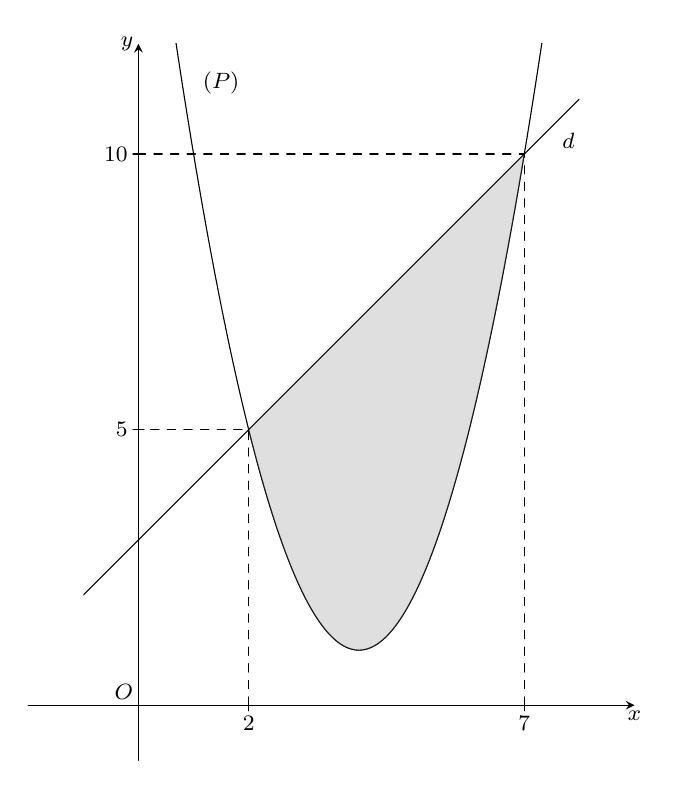
\begin{tikzpicture}[scale=.7,>=stealth,line cap=round,line join=round,font=\footnotesize]
				 \def\f (#1){(#1)^2-8*(#1)+17}
				\def\g (#1){(#1)+3} 
				\def\xmin{-1} 
				\def\xmax{8} 
				\def\ymin{-1} 
				 \def\ymax{12}
				 \draw[->] (\xmin-1,0)--(\xmax+1,0) node[below] {$x$};
				\draw[->] (0,\ymin)--(0,\ymax) node[left]  {$y$};
				\draw (0,0) node [above left]  {$O$};
				\clip  (\xmin,\ymin) rectangle (\xmax,\ymax);
				\foreach \x in {2,7}\draw (\x,0.1)--(\x,-0.1) node  [below] {$\x$};
				\foreach  \y in {5,10}\draw (0.1,\y)--(-0.1,\y) node [left] {$\y$};
				\draw[smooth,samples=200] plot[domain=\xmin:\xmax]  (\x,{\f (\x)});
				\draw[smooth,samples=200] plot[domain=\xmin:\xmax] (\x,{\g (\x)}); 
				 \draw[fill=gray!50!white,opacity=0.5] plot[domain=2:7] (\x,{\f (\x)})--plot[domain=7:2](\x,{\g (\x)});
				\draw  (1.5,11) node[above]{$(P)$}
					(7.8,10)  node[above]{$d$};
				 \draw[dashed] (2,0)--(2,5)--(0,5)
					(7,0)--(7,10)--(0,10); 

			\end{tikzpicture}
	\end{center}
	\choice 
		{\True $\dfrac{215}{3}$} 
		 {$\dfrac{265}{3}$}
		 {$\dfrac{245}{3}$}
		 {$\dfrac{415}{3}$}
	\loigiai{ 
		Dựa vào đồ thị  ta có điểm $A(2;5)$ và $B(7;10)$ thuộc đường thẳng $d$ và Parabol $(P)$.\\
		Suy ra  đường thẳng $d$ có vecto chỉ phương $\vec{AB} = (5;5)$.
		Phương trình  đường thẳng $d: y = x + 3$.\\
		Gọi $(P)$ có phương trình $y = ax^2 + bx + c,  (a > 0)$.\\
		$A, B \in (P)$  suy ra ta có hệ phương trình
		\begin{eqnarray*}
			& & \begin{cases} 4a + 2b + c = 5 \\ 49a + 7b + c = 10
		\end{cases}\\
		&\Leftrightarrow & \begin{cases} c = -4a - 2b + 5 \\ 49a + 7b + 5 - 4a - 2b = 10
	\end{cases}\\
	&\Leftrightarrow & \begin{cases} c = -4a - 2b + 5 \\ 45a + 5b = 5
	\end{cases}\\
	&\Leftrightarrow & \begin{cases} c = -4a - 2b + 5 \\ 9a + b = 1
	\end{cases}\\
	&\Leftrightarrow &\begin{cases} c = 3 + 14a \\ b = 1 - 9a.
	\end{cases}
	\end{eqnarray*}
	Hình phẳng  giới hạn bởi $(P)$ và $d$ có diện tích $S = \dfrac{125}{6}$.
	 Suy ra
	\begin{eqnarray*}
		& &\displaystyle\int_{2}^{7}  |x + 3 - (ax^2 + bx + c)| \mathrm{\,d}x= \dfrac{125}{6}\\
		&\Leftrightarrow & \displaystyle\int_{2}^{7} |x  + 3 - [ax^2 + (1 - 9a)x + (3 + 14a)]| \mathrm{\,d}x = \dfrac{125}{6}\\
		&\Leftrightarrow & \displaystyle\int_{2}^{7} |-ax^2  + 9ax - 14a| \mathrm{\,d}x = \dfrac{125}{6} \\
		 &\Leftrightarrow & \left| -a \left( \dfrac{x^3}{3} - \dfrac{9x^2}{2} + 14x \right) \right|_{2}^{7} = \dfrac{125}{6}\\
		&\Leftrightarrow & \left| -a \left( \left( \dfrac{7^3}{3} - \dfrac{9 \cdot 7^2}{2} + 14 \cdot 7 \right) -  \left( \dfrac{2^3}{3} - \dfrac{9 \cdot 2^2}{2} + 14 \cdot 2 \right) \right) \right| = \dfrac{125}{6}\\
		&\Leftrightarrow  & \left| -a \left( \dfrac{343}{3} - \dfrac{441}{2} + 98 - \left( \dfrac{8}{3} - 18 + 28 \right) \right) \right| = \dfrac{125}{6}\\
		&\Leftrightarrow & \left| -a \left( \dfrac{343}{3} - \dfrac{441}{2} + 98 - \dfrac{8}{3} + 18 - 28 \right) \right|  = \dfrac{125}{6}\\
		&\Leftrightarrow & \left| -a \left( \dfrac{335}{3} -  \dfrac{441}{2} + 88 \right) \right| = \dfrac{125}{6}
		 \Leftrightarrow \left| -a \left( \dfrac{670 - 1323 + 528}{6} \right) \right| = \dfrac{125}{6}\\
		&\Leftrightarrow & \left| -a \left(  -\dfrac{125}{6} \right) \right| = \dfrac{125}{6}\\
		&\Leftrightarrow & \dfrac{125}{6} |a| =  \dfrac{125}{6} \Leftrightarrow a = 1.
	\end{eqnarray*}
	$a = 1 \Rightarrow b = -8; c = 17$.\\ 
	$(P)$ có phương trình $y = f(x) = x^2 - 8x  + 17$.\\
	Suy ra $f'(x) = 2x  - 8 \Rightarrow \displaystyle\int_{2}^{7} (2x - 3)f'(x) \mathrm{\,d}x = \dfrac{215}{3}$.
} 
\end{ex}

% nguồn: Phan1_Lop_12_Dai_so_Chuong_4
\begin{ex}%[2D4V3-1]%[ma:53d2ecc2]
	\immini{Cho hàm  số $y=f(x)$ thỏa mãn hàm số $y=f^{\prime}(x)$ liên tục trên $\mathrm{R}$ và có đồ thị như hình bên. Giá trị của biểu thức $f(4)-f(-4)$ bằng
	 \choice
		 {\True $12$}
		{$3$} 
		{$24$} 
		{$6$} 
		}{\resizebox{0.5\linewidth}{!}{\begin{tikzpicture}[line join=round,line cap=round,>=stealth]
		\draw[->](-5,0)--(6,0) node[below]  {$x$};
		 \draw[->](0,-1.5)--(0,4) node[right] {$y$};
		\node  (0,0) [below right]{$O$};
		\foreach \x/\g in  {-4/-90,-3/-90,-2/-90,-1/-90,1/-90,2/-90,3/-90,4/-90}
		\draw[thin] (\x,2pt)--(\x,-2pt) + (\g:4mm) node {\scriptsize  $\x$};
		\foreach \y/\g  in {-1/0,1/0,2/0,3/180}
		\draw[thin] (2pt,\y)--(-2pt,\y) + (\g:4mm) node {\scriptsize  $\y$};
		 \draw[dashed] (1,0)--(1,3)--(0,3);
		 \draw (-4.833,-0.5)--(-4,0)--(1,3)--(5,-1);
		 \draw (2,2) node[right] {$y=f^{\prime}
			(x)$}; 
	\end{tikzpicture}}
		 }
	\loigiai{ 
		 $f(4)-f(-4)=\displaystyle\int_{-4}^{4} f^{\prime}(x) \mathrm{\,d}x=\displaystyle\int_{-4}^{1} f^{\prime}(x) \mathrm{\,d}x+\displaystyle\int_{1}^{4} f^{\prime}(x) \mathrm{\,d}x=\dfrac{1}{2} \cdot 5 \cdot 3+\dfrac{1}{2} \cdot 3 \cdot 3=12$.
	 }
\end{ex}


%%%%%%%%%%%%%%%% ĐÚNG/SAI %%%%%%%%%%%%%%%%

% nguồn: Phan1_Lop_12_Dai_so_Chuong_4
\begin{ex}%[2D4H3-1]%[ma:0df7f67b]
	Cho hàm số $y=\sqrt{2-x}$ có đồ thị $(H)$ và đường thẳng $y=2x-2$.  Khi đó
	\choiceTF 
		{Diện tích hình phẳng $D$ giới hạn bởi đồ  thị $(H)$, trục tung, trục hoành là $\int_{0}^{2} (\sqrt{2-x}) dx$}
		{Diện tích hình phẳng giới  hạn bởi đồ thị $(H)$, $x=-1$ và trục hoành là $\dfrac{2\sqrt{9}}{3}$}
		{\True Thể tích khối tròn xoay  tạo thành khi quay hình phẳng $D$ quanh trục $Ox$ là $2\pi$ (đvtt)}
		 {\True Giá trị $\dfrac{a\sqrt{3}+b\sqrt{2}+c}{3}$ là diện tích hình phẳng giới hạn bởi đồ thị $(H)$ và các đường thẳng $x=0, x=-1, y=2x-2$. Khi đó $a+b+c=11$}
	 \loigiai{
		\begin{itemchoice}
			 \itemch Diện tích hình phẳng $D$ giới hạn bởi đồ thị $(H)$, trục tung, trục hoành là\\
			$S = \displaystyle\int_{0}^{2}  |\sqrt{2-x}| dx = \displaystyle\int_{0}^{2} \sqrt{2-x}.dx$
			\itemch Diện tích cần tìm là\\ $S = \displaystyle\int_{-1}^{2}\sqrt{2-x}dx = \displaystyle\int_{-1}^{2} (2-x)^{\tfrac{1}{2}}dx = -\dfrac{2}{3}(2-x)^{\tfrac{3}{2}}\Big|_{-1}^{2} \\=  -\dfrac{2}{3}(2-2)^{\tfrac{3}{2}} - (-\dfrac{2}{3}(2-(-1))^{\tfrac{3}{2}}) = \dfrac{2}{3}(3)^{\tfrac{3}{2}} = \dfrac{2}{3}(3\sqrt{3}) = 2\sqrt{3}$.
			\itemch Thể tích khối tròn  xoay tạo thành khi quay hình phẳng $D$ quanh trục $Ox$ là\\
			$V = \pi \displaystyle\int_{0}^{2} (\sqrt{2-x})^2 dx =  2\pi$.
			\itemch Diện  tích cần tìm là\\ $S = \displaystyle\int_{-1}^{0} |\sqrt{2-x}-(2x-2)|dx = \displaystyle\int_{-1}^{0} (\sqrt{2-x}-(2x-2))dx \\= \left[-\dfrac{2}{3}(2-x)^{\tfrac{3}{2}}-(x^2-2x)\right]_{-1}^{0}$
			$=-\dfrac{2}{3}2\sqrt{2} - \left(-\dfrac{2}{3}3\sqrt{3}-(1+2)\right) = -\dfrac{4\sqrt{2}}{3} + 2\sqrt{3} + 3 =  \dfrac{6\sqrt{3}-4\sqrt{2}+9}{3}$\\
			Khi đó ta có $a = 6, b =  -4, c =9$, $a+b+c=11$.
		\end{itemchoice}
	} 
\end{ex}

% nguồn: Phan1_Lop_12_Dai_so_Chuong_4
\begin{ex}%[2D4H3-1]%[ma:2fdf9008]
	 \immini{
	Cho hàm số $y=f(x)$ liên tục trên đoạn $[0;5]$ và có đồ thị trên đoạn $[0;5]$ là đường gấp khúc $ABCD$ như hình vẽ. 
	 \choiceTF
		{\True Diện tích  hình thang $OABC$ bằng $5$ và diện tích tam giác $CDE$ bằng $1$}
		{\True  $\displaystyle\int_0^3f(x)\mathrm{\,d}x=5$}
		 {$\displaystyle\int_3^5f(x)\mathrm{\,d}x=1$}
		 {\True $\displaystyle\int_0^5f(x)\mathrm{\,d}x=4$}}
		 {
		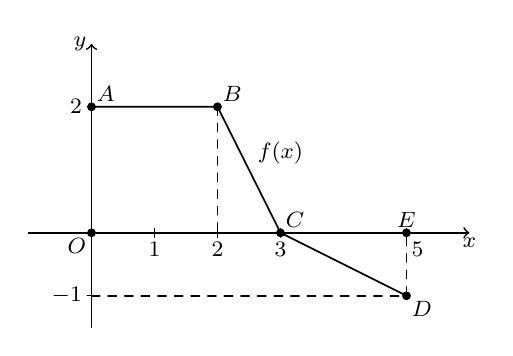
\begin{tikzpicture}[line join=round,line cap=round,line width=.6pt,font=\footnotesize,scale=.8]
				\draw[->] (-1,0) -- (6,0) node[below] {$x$}; 
				\draw[->] (0,-1.5) --  (0,3) node[left] {$y$};
				\foreach \x in {1,2,3}  \draw[thin] (\x,2pt)--(\x,-2pt) node [below] {$\x$};
				 \foreach \y in {-1,2} \draw[thin] (2pt,\y)--(-2pt,\y) node [left] {$\y$};
				\draw[thin] (5,2pt)--(5,-2pt)  node [below right] {$5$};
				\coordinate[label=below  left:$O$](O) at (0,0);
				\coordinate[label=above right:$A$](A) at (0,2); 
				\coordinate[label=above right:$B$](B) at (2,2); 
				\coordinate[label=above right:$C$](C) at  (3,0);
				 \coordinate[label=above:$E$](E) at (5,0);
				 \coordinate[label=below right:$D$](D) at (5,-1);
				\coordinate[label=above:$f (x)$](X) at (3,1); 
				\foreach \a in {A,B,C,E,D,O}  \fill (\a) circle (2pt);
				\draw  (A)--(B)--(C)--(D);
				\draw [dashed] (2,2)--(2,0) 
					(0,-1)--(5,-1)--(5,0); 
			\end{tikzpicture}
		 }
	 \loigiai{
		\begin{itemchoice}
			\itemch Ta có $S_{OABC}=\dfrac{AB+OC}{2}\cdot OA=\dfrac{2+3}{2}\cdot  2=5$.\\
			$S_{CDE}=\dfrac{1}{2}\cdot EC \cdot DE=\dfrac{1}{2}\cdot 2 \cdot  1=1$.
			 \itemch Ta có $\displaystyle\int_0^3f(x)\mathrm{\,d}x=S_{OABC}=5$.
			 \itemch Ta có $\displaystyle\int_3^5f(x)\mathrm{\,d}x=-S_{CDE}=-1$.
			 \itemch Ta có $\displaystyle\int_0^5f(x)\mathrm{\,d}x=S_{OABC}-S_{CDE}=5-1=4$.
		\end{itemchoice}
	} 
\end{ex}

% nguồn: Phan1_Lop_12_Dai_so_Chuong_4
\begin{ex}%[2D4H3-1]%[ma:3c3d7b95]
	Trong mặt phẳng $Oxy$, cho hàm số $y=x+\sqrt x $ và  $y=x+x^2$. \choiceTF
	{Hoành độ giao điểm của đồ thị hai hàm số trên  là $x=0$ hoặc $x=-1$}
	{\True Diện tích hình phẳng giới hạn bởi đồ thị hai  hàm số trên và $x=0$, $x=1$ được tính theo công thức $S=\displaystyle\int_0^1\left(\sqrt x-x^2\right){\rm{d}}x$}
	{Diện tích hình phẳng giới hạn bởi đồ thị  hai hàm số trên và $x=0$, $x=1$ được tính theo công thức $S=\displaystyle\int_0^1\left(x+x^2\right){\rm{d}}x-\displaystyle\int_0^1\left(x+\sqrt x\right){\rm{d}}x$}
	{\True Diện tích hình phẳng giới hạn bởi  đồ thị hai hàm số trên và $x=0$, $x=1$ bằng $\dfrac{1}{3}$ (đvdt)}
	 \loigiai{
		\begin{itemchoice}
			\itemch Phương trình hoành giao độ giao điểm của hai đồ thị hàm số  trên là
			$$x+\sqrt x=x+x^2\Leftrightarrow x=x^4 \Leftrightarrow\hoac{&x=0\\&  x=1.}$$
			\itemch Diện tích hình phẳng được giới  hạn bởi các đường $y=x+\sqrt x $, $y=x+x^2$, $x=0$, $x=1$ là $$S=\displaystyle\int_0^1\left|\left(x+\sqrt x\right)-\left(x+x^2\right)\right|\rm{d}x =\displaystyle\int_0^1\left|\sqrt x-x^2\right|\rm{d}x =\displaystyle\int_0^1\left(\sqrt x-x^2\right){\rm{d}}x$$
			\itemch Diện tích hình phẳng được giới hạn bởi các  đường $y=x+\sqrt x $, $y=x+x^2$, $x=0$, $x=1$ là
			\begin{eqnarray*}
				 S&=&\displaystyle\int_0^1\left|\left(x+\sqrt x\right)-\left(x+x^2\right)\right|\rm{d}x\\
				&=&\displaystyle\int_0^1\left[\left(x+\sqrt x\right)-\left(x+x^2\right)\right]{\rm{d}}x\quad (\text{vì}\quad  x+\sqrt x\ge x+x^2\, ,\forall x\in\left[0; 1\right])\\
				&=&\displaystyle\int_0^1\left(x+\sqrt  x\right){\rm{d}}x-\displaystyle\int_0^1\left(x+x^2\right){\rm{d}}x.
			\end{eqnarray*}
			\itemch Diện tích hình  phẳng được giới hạn bởi các đường $y=x+\sqrt x $, $y=x+x^2$, $x=0$, $x=1$ là $$S=\displaystyle\int_0^1\left(\sqrt x-x^2\right){\rm{d}}x \left.=\left(\dfrac{2}{3}{x^{\tfrac{3}{2}}}-\dfrac{x^3}{3}\right)\right|_0^1 =\dfrac{2}{3}-\dfrac{1}{3}=\dfrac{1}{3} \,(\text{đvdt}).$$
		\end{itemchoice}
	} 
\end{ex}

% nguồn: Phan1_Lop_12_Dai_so_Chuong_4
\begin{ex}%[2D4H3-1]%[ma:f45f3891]
	Trong mặt phẳng tọa độ  $Oxy$, xét parabol $(P)\colon y=x^2-4$.
	\choiceTF 
		{\True Hoành độ  giao điểm của $(P)$ và $Ox$ là $-2$ và $2$}
		 {$\displaystyle\int(x^2-4)\mathrm{\,d}x=\dfrac{x^3}{3}+4x+C$}
		{$\left|x^2-4\right|=x^2-4$, $\forall  x\in [-2;2]$}
		 {\True Diện tích hình phẳng giới hạn bởi $(P)$ và $Ox$ bằng $\dfrac{32}{3}$}
	\loigiai{ 
		\begin{itemchoice}
			 \itemch {\bf Đúng}.\\
			 Vì $x^2-4=0\Leftrightarrow x=\pm 2$.
			\itemch {\bf  Sai}.\\
			 Vì $\displaystyle\int \left(x^2-4\right)\mathrm{\,d}x=\dfrac{x^3}{3}-4x+C$.
			\itemch  {\bf Sai}.\\
			Vì giả sử $x=0\in [-2;2]$ thì $|x^2-4|=|0-4|=4$ và  $x^2-4=0-4=-4$.
			 \itemch {\bf Đúng}.\\
			Vì diện tích hình phẳng giới hạn bởi $(P)$ và  $Ox$ là \[S=\displaystyle\int_{-2}^2\left|x^2-4\right|\mathrm{\,d}x=-\left(\dfrac{x^3}{3}-4x\right)\Bigg|_{-2}^2=\dfrac{32}{3}.\]
		\end{itemchoice}
	} 
\end{ex}

% nguồn: Phan1_Lop_12_Dai_so_Chuong_4
\begin{ex}%[2D4H3-1]%[ma:f9b322fb]
	Cho hàm số $y=x^3-3x+2$ đồ thị là $(C)$ và đường thẳng $y=-2x+8$ có đồ thị là $(d)$ và các đường thẳng $x=1$, $x=3$. Gọi $S_1$ là diện tích hình phẳng giới hạn bởi  $(d)$, trục hoành và đường thẳng $x=1$, $x=3$. Gọi $S_2$ là diện tích hình phẳng giới hạn bởi $(d)$, trục hoành và đường thẳng $x=5$. Xét tính đúng sai của các khẳng định sau
	 \choiceTF
		 {Số giao điểm của đồ thị $(C)$ và đường thẳng $(d)$ là $3$}
		{Hàm số $y=x^3-3x+2$ đạt cực tiểu  tại $x=1$}
		{\True $S_1 >  S_2$}
		{Diện tích hình phẳng  giới hạn bởi hai đồ thị hàm số $y=x^3-3x+2$, $y=-2x+8$ và hai đường thẳng $x=1, x=3$ bằng $23$}
	 \loigiai{
		\begin{enumerate}
			\item \textbf{Sai.} Phương trình hoành độ giao điểm \\ $x^3-3x+2=-2x+8 \Leftrightarrow x^3-x-6=0 \Leftrightarrow  x=2$.\\
			 Vậy chỉ có 1 giao điểm.
			\item \textbf{Đúng.} Xét $y=x^3-3x+2$. Ta có $y'=3x^2-3$. 
			$y'=0 \Leftrightarrow  x=\pm 1$.
			\begin{center}
				
\begin{tikzpicture}
						 \tkzTabInit[lgt=3]
						{$x$/1,$3x^2-3$/1} 
						{$-\infty$,$-1$,$1$,$+\infty$} 
						 \tkzTabLine{,+,0,-,0,+,}
					\end{tikzpicture}
			\end{center}
			Vậy hàm số đạt cực  tiểu tại $x=1$.
			\item \textbf{Đúng.} Đường  thẳng $(d)\colon y=-2x+8$ cắt trục hoành tại $x=4$.
			\begin{itemize}
				\item $S_1 = \displaystyle\int_1^4 |-2x+8|\mathrm{d}x = \int_1^4 (-2x+8)\mathrm{d}x =9$. 
				\item $S_2$ là diện tích giới hạn bởi $(d)$, trục hoành,  và $x=5$. \\
				$S_2 = \displaystyle\int_4^5  |-2x+8|\mathrm{d}x = \int_4^5 (2x-8)\mathrm{d}x = 1$.
			\end{itemize}
			Vậy  $S_1 > S_2$.
			\item  \textbf{Sai.} Diện tích cần tính là $A = \displaystyle\int_1^3 |(x^3-3x+2)-(-2x+8)|\mathrm{d}x = \int_1^3|x^3-x-6|\mathrm{d}x$.
			\\ Vì $x^3-x-6 < 0$ trên  $[1;2)$ và $x^3-x-6>0$ trên $(2;3]$, nên \\
			$A = \displaystyle\int_1^2(-x^3+x+6)\mathrm{d}x  + \int_2^3(x^3-x-6)\mathrm{d}x= 11{,}5$.
		\end{enumerate}
	 }
\end{ex}

% nguồn: Phan1_Lop_12_Dai_so_Chuong_4
\begin{ex}%[2D4H3-1]%[ma:3b816c17]
	 Cho hàm số $f(x)=\mathrm{e}^x-1$.
	\choiceTF 
		{\True Họ nguyên hàm của hàm  số là $\mathrm{e}^x-x+C$ (với $C$ là hằng số)}
		 {\True Gọi $F(x)$ là một nguyên hàm của $f(x)$ trên $\mathbb{R}$, với $F(0)=3$ thì $F(x)=\mathrm{e}^x-x+2$}
		{Cho $\displaystyle\int_0^1g(x)\mathrm{\,d}x=7$, ta có  $\displaystyle\int_0^1[f(x)+g(x)]\mathrm{\,d}x=7\mathrm{e}$}
		{\True Diện tích  hình phẳng giới hạn bởi đồ thị hàm số $y=f(x)$, trục $Ox$ và đường thẳng $x=2$ bằng $\mathrm{e}^2-3$}
	\loigiai{\begin{itemchoice}
		\itemch Ta có $\displaystyle\int  f(x)\mathrm{\,d}x=\displaystyle\int\left(\mathrm{e}^x-1\right)\mathrm{d}x=\mathrm{e}^x-x+C$.
		 \itemch Có $F(x)=\displaystyle\int f(x)\mathrm{\,d}x=\mathrm{e}^x-x+C$.\\
		 Do $F(0)=3$ nên $1+C=3\Leftrightarrow C=2$.\\
		Suy ra $F(x)=\mathrm{e}^x-x+2$. 
		\itemch Ta  có $\displaystyle\int_0^1[f(x)+g(x)]\mathrm{\,d}x=\displaystyle\int_0^1f(x)\mathrm{\,d}x+\displaystyle\int_0^1g(x)\mathrm{\,d}x=\left(\mathrm{e}^x-x\right)\bigg|_0^1+7=\mathrm{e}+5$.
		\itemch Phương trình hoành độ giao điểm  của đồ thị hàm số với trục hoành là
		 \[\mathrm{e}^x-1=0\Leftrightarrow\mathrm{e}^x=1\Leftrightarrow x=0.\]
		Diện tích hình  phẳng cần tìm là
		\[S=\displaystyle\int_0^2\left|\mathrm{e}^x-1\right|\mathrm{\,d}x=\displaystyle\int_0^2\left(\mathrm{e}^x-1\right)\mathrm{\,d}x=\left(\mathrm{e}^x-x\right)\bigg|_0^2=\mathrm{e}^2-3.\] 
\end{itemchoice}}
\end{ex}

% nguồn: Phan1_Lop_12_Dai_so_Chuong_4
\begin{ex}%[2D4H3-1]%[ma:6df224b6]
	Cho hai hàm số  $f(x)=2x^2$ và $F(x)=\dfrac{2x^3}{3}$.
	\choiceTF 
		{\True Ta có $f(x)\geq0$, $\forall x\in\mathbb{R}$} 
		{\True Hàm số $F(x)$ là một nguyên hàm của hàm  số $f(x)$ trên $\mathbb{R}$}
		{Tích phân từ $1$ đến $3$ của hàm số $f(x)$ là  $\displaystyle\int_1^3f(x)\mathrm{\,d}x=F(1)-F(3)$}
		{Hình phẳng giới hạn bởi đồ thị hàm số $y=f(x)$, trục hoành và hai đường  thẳng $x=1$, $x=3$ có diện tích bằng $18$}
	\loigiai{ 
		\begin{itemchoice}
			\itemch  \textbf{Đúng}. Ta có $f(x)=2x^2\ge 0,\forall x\in\mathbb{R}$.
			\itemch \textbf{Đúng}. Ta có $F'(x)=2x^2$. Do đó $F(x)$ là một nguyên hàm của $f(x)$  trên $\mathbb{R}$.
			\itemch  \textbf{Sai}. Tích phân từ $1$ đến $3$ của hàm số $f(x)$ là $\displaystyle\int_1^3f(x)\mathrm{\,d}x=F(3)-F(1)$.
			\itemch \textbf{Sai}. Hình phẳng giới hạn bởi đồ thị hàm số $y=f(x)$, trục hoành và hai đường  thẳng $x=1$, $x=3$ là
			\[S=\displaystyle\int_1^3\left|f(x)\right|\mathrm{\,d}x=\displaystyle\int_1^3\left|2x^2\right|\mathrm{\,d}x=\dfrac{2}{3}x^3\Bigg|_1^3=18-\dfrac{2}{3}=\dfrac{52}{3}.\] 
		\end{itemchoice}
	 }
\end{ex}

% nguồn: Phan1_Lop_12_Dai_so_Chuong_4
\begin{ex}%[2D4H3-1]%[ma:f0566c23]
	Cho hàm số $y=f(x)$ có đạo hàm $f'(x)$ và $f''(x)$ liên tục trên khoảng $(0;+\infty)$, có bảng biến  thiên như sau
	\begin{center}
		
\begin{tikzpicture}[font=\footnotesize,line join=round,line cap=round,>=stealth,scale=1]
				 \tkzTabInit[lgt=1.2,espcl=2.5,nocadre=false]
					{$x$ /0.7,$y'$ /0.7,$y$ /2} 
					 {$0$,$2$,$3$,$5$,$+\infty$}
				 \tkzTabLine{,+,z,-,z,+,z,-,}
				\tkzTabVar{-/$-\infty$,+/$0$,-/$-1$,+/$f  (5)$,-/$-\infty$}
			\end{tikzpicture}
	\end{center}
	 \choiceTF
		{\True $\displaystyle\int_2^5 f'(x)\mathrm{\,d}x=f(5)-f(2)$} 
		{$\displaystyle\int_2^3 f'(x)\mathrm{\,d}x=1$} 
		{Diện tích hình phẳng giới hạn bởi đồ thị $(C)\colon y=f'(x)$; $y=0$; $x=2$; $x=3$ bằng  $\dfrac{1}{2}$}
		{Biết rằng $\displaystyle\int_2^5  \left|f'(x)\right|\mathrm{\,d}x=5$, suy ra $f(5)=5$}
	 \loigiai{
		\begin{itemchoice}
			\itemch Ta có $\displaystyle\int_2^5 f'(x)\mathrm{\,d}x=f(x)\Big|_2^5=f(5)-f(2)$. 
			 \itemch Ta có $\displaystyle\int_2^3 f'(x)\mathrm{\,d}x=f(x)\Big|_2^3=f(3)-f(2)=-1-0=-1$.
			 \itemch Diện tích hình phẳng là
			 $$S=\displaystyle\int_2^3 \left|f'(x)\right| \mathrm{\,d}x=-\displaystyle\int_2^3 f'(x)\mathrm{\,d}x=-f(x)\Big|_2^3=-f(3)+f(2)=1+0=1.$$
			\itemch  Ta có
			\begin{eqnarray*}
				 &&\displaystyle\int_2^5 \left|f'(x)\right|\mathrm{\,d}x=5\\
				 &\Leftrightarrow&\displaystyle\int_2^3 \left|f'(x)\right|\mathrm{\,d}x+\displaystyle\int_3^5 \left|f'(x)\right|\mathrm{\,d}x=5\\
				&\Leftrightarrow&1+f(5)-f(3)=5\\ 
				 &\Leftrightarrow& 1+f(5)-(-1)=5\\
				&\Leftrightarrow& f(5)=3. 
			\end{eqnarray*}
		\end{itemchoice}
	 }
\end{ex}

% nguồn: Phan1_Lop_12_Dai_so_Chuong_4
\begin{ex}%[2D4H3-1]%[ma:8894a5bb]
	Cho đồ thị hàm số $y=x^3-2x^2-3x+4$ có đồ thị  $(C)$ và đường thẳng $(d) \colon y=2x-2$. Xét tính đúng sai của các khẳng định sau
	\begin{center}
		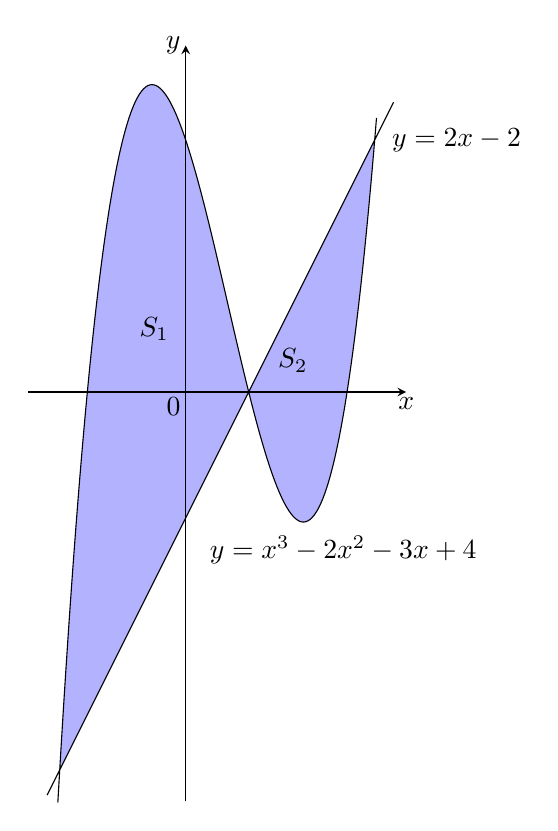
\begin{tikzpicture}[scale=.8]
				\def\hsf  (#1){(#1)^3-2*(#1)^2-3*(#1)+4}
				\def\hsg (#1){2*(#1)-2} 
				 \fill[blue!30]
					 plot[domain=-2:3] (\x,{\hsf (\x)})
					plot[domain=3:-2] (\x,{\hsg (\x)}); 
				\draw[smooth] 
					plot[domain=-2.03:3.03] (\x,{\hsf (\x)}) 
					plot[domain=-2.2:3.3]  (\x,{\hsg (\x)});
				\draw[-stealth] (-2.5,0)--(0,0) node[below  left]{$0$}--(3.5,0) node[below]{$x$};
				\draw[-stealth] (0,-6.5)--(0,5.5) node[left]{$y$}; 
				\node  at (-0.5,1){$S_1$};
				\node  at (1.7,0.5){$S_2$};
				\node at  (4.3,4){$y=2x-2$};
				 \node at (2.5,-2.5){$y=x^3-2x^2-3x+4$};
			\end{tikzpicture}
	\end{center}
	\choiceTF 
		{\True Đường thẳng $d$ cắt đồ  thị $(C)$ tại ba điểm $A(-2;-6)$, $B(1;0)$, $C(3;4)$}
		{Diện tích hình phẳng giới hạn bởi đồ thị $(C)$, trục hoành, đường thẳng $x=-1; x=2$ bằng  $\dfrac{21}{4}$}
		 {\True Diện tích hình phẳng giới hạn bởi đồ thị $(C)$ và đường thẳng $d$ bằng $\dfrac{253}{12}$}
		{Biết đường thẳng $d$ cắt đồ thị $(C)$ thành hai miền $S_1$ và $S_2$.  Khi đó tỉ số $\dfrac{S_1}{S_2}=\dfrac{63}{16}$}
	\loigiai{ 
		\begin{enumerate}
			\item \textbf{Đúng.} 
			Phương trình hoành độ giao  điểm $$x^3-2x^2-3x+4=2x-2 \Leftrightarrow x^3-2x^2-5x+6=0 \Leftrightarrow \hoac{x&=-2 \Rightarrow y=-6. \\ x&=1 \Rightarrow y=0. \\ x&=3 \Rightarrow y=4.}$$
			 Vậy có 3 giao điểm đúng như khẳng định.
			\item \textbf{Sai.} 
			Diện tích cần tính là \\ $$S = \displaystyle\int_{-1}^2 |x^3-2x^2-3x+4|\mathrm{d}x= \displaystyle\int_{-1}^1 (x^3-2x^2-3x+4)\mathrm{d}x - \int_1^2 (x^3-2x^2-3x+4)\mathrm{d}x  =\dfrac{97}{12}.$$
			 \item \textbf{Đúng.}
			Diện tích giới hạn bởi $(C)$ và $(d)$ là $$S=S_1+S_2= \displaystyle\int_{-2}^1 (x^3-2x^2-5x+6)\mathrm{d}x + \int_1^3  -(x^3-2x^2-5x+6)\mathrm{d}x= \dfrac{253}{12}.$$
			\item  \textbf{Sai.}
			Ta $\dfrac{S_1}{S_2} =\dfrac{\dfrac{63}{4}}{\dfrac{16}{3}} = \dfrac{189}{64}$. 
		\end{enumerate}
	} 
\end{ex}

% nguồn: Phan1_Lop_12_Dai_so_Chuong_4
\begin{ex}%[2D4H3-1]%[ma:aaedc6c4]
	Cho hàm số $f(x)=\dfrac{2 x^{2}+1}{x}$ có đồ thị  $(C)$
	\choiceTF 
		{\True Họ nguyên hàm của hàm số  $f(x)$ trên $(0;+\infty)$ là $x^{2}+\ln x+C$}
		{\True Giá  trị của tích phân $\displaystyle\int_{1}^{2} 3 x f(x) \mathrm{\,d}x$ bằng $17$}
		{Diện tích hình phẳng $(H)$  giới hạn bởi đồ thị $(C)$ và đường thẳng $y=-3$ được tính bởi công thức $\displaystyle\int_{-1}^{-\tfrac{1}{2}}|f(x)-3| \mathrm{\,d}x$}
		{\True Hình phẳng $(G)$ giới hạn bởi $(C)$ và đường thẳng $d\colon y=3$ quay quanh trục  $O x$ tạo thành khối tròn xoay có thể tích bằng $\dfrac{\pi}{3}$}
	\loigiai{ 
		\begin{itemchoice}
			\itemch  $\displaystyle\int {f(x)\mathrm{\,d}x}=\displaystyle\int {\dfrac{2x^2+1}{x}\mathrm{\,d}x}=\displaystyle\int {\left(2x+\dfrac{1}{x}\right)\mathrm{\,d}x}=x^2+\ln x + C.$
			\itemch $\displaystyle\int_{1}^{2} 3 x f(x)  \mathrm{\,d}x=\displaystyle\int_{1}^{2} 3 x \cdot \dfrac{2x^2+1}{x} \mathrm{\,d}x=\displaystyle\int_{1}^{2} \left(6x^2+3\right) \mathrm{\,d}x=\left(2x^3+3x\right) \biggl|_1^2=22-5=17$.
			\itemch Diện tích hình phẳng $(H)$ giới hạn bởi đồ thị $(C)$ và đường thẳng $y=-3$  được tính bởi công thức $\displaystyle\int_{-1}^{-\tfrac{1}{2}}\left|f(x)-(-3)\right| \mathrm{\,d}x=\displaystyle\int_{-1}^{-\tfrac{1}{2}}\left|f(x)+3\right| \mathrm{d\,}x.$
			\itemch Phương trình hoành độ giao điểm của hai đường 
			$$  \dfrac{2x^2+1}{x}=3 \Leftrightarrow 2x^2-3x+1 =0 \Leftrightarrow \hoac{&x=\dfrac{1}{2}\\&x=1.}$$
			Thể tích của hình $(G)$  khi xoay quanh $Ox$ là
			$$V=\pi \displaystyle\int_{\tfrac{1}{2}}^{1} \left|3^2-\left(\dfrac{2x^2+1}{x}\right)^2\right| \mathrm{\,d}x=\dfrac{\pi}{3}.$$ 
		\end{itemchoice}
	 }
\end{ex}

% nguồn: Phan1_Lop_12_Dai_so_Chuong_4
\begin{ex}%[2D4V3-1]%[ma:2c44eca5]
	Cho hàm số bậc  hai $y=-x^2+5x$ và đường thẳng $y=2x$.
	 \choiceTF
		{\True Tọa độ giao  điểm của đường thẳng $y=2x$ và đồ thị hàm số $y=-x^2+5x$ là $A\left(0;0\right)$ và $B\left(3;6\right)$}
		{Diện tích hình phẳng giới hạn bởi đồ thị hàm số $y=-x^2+5x$ và trục  hoành là $\dfrac{27}{2}$}
		{\True Diện tích hình phẳng giới hạn bởi đồ thị hàm  số $y=-x^2+5x$ và $y=2x$ là $\dfrac{9}{2}$}
		{Gọi $S_1$ là diện tích hình phẳng giới hạn bởi đồ thị hàm số $y=-x^2+5x$; $y=2x$ và $S_2$  là diện tích hình phẳng giới hạn bởi đồ thị hàm số $y=-x^2+5x$; $y=2x$ với trục hoành. Tỉ số diện tích $\dfrac{S_1}{S_2}$ bằng $\dfrac{27}{6}$}
	\loigiai{ 
		\begin{itemchoice}
			\itemch 
			 Phương trình hoành độ giao điểm của đồ thị hàm số $y=-x^2+5x$ và đường thẳng $y=2x$ là $-x^2+5x=2x \Leftrightarrow
			\hoac{&x=0\\&x=3.}$\\ Khi đó ta có hai  giao điểm là $A\left(0;0\right)$ và $B\left(3;6\right)$.
			 \itemch
			Diện tích hình phẳng giới hạn bởi đồ thị hàm số $y=-x^2+5x$  với trục hoành là
			 $$S=\displaystyle\int_{0}^{5}\left|-x^2+5x\right|\,\mathrm{d}x=\dfrac{125}{6}.$$
			\itemch 
			Diện tích hình phẳng giới hạn bởi đồ thị hàm số $y=-x^2+5x$  và $y=2x$ là
			$$S_1=\displaystyle\int_{0}^{3}\left|-x^2+3x\right|\,\mathrm{d}x=\dfrac{9}{2}.$$ 
			\itemch 
			Ta có $S_2=S-S_1=\dfrac{125}{6}-\dfrac{9}{2}=\dfrac{49}{3}$.\\  Khi đó $\dfrac{S_1}{S_2}=\dfrac{27}{98}$.
		\end{itemchoice}
	} 
\end{ex}


%%%%%%%%%%%%%%%% TRẢ LỜI NGẮN %%%%%%%%%%%%%%%%

% nguồn: Phan2_Lop_12_Dai_so_Chuong_4
\begin{bt}%[2D4N3-1]%[ma:0084e64a]
	\immini[thm]{Đồ thị trong hình dưới đây là của hàm số $y=f(x)$. Biết $\displaystyle\int_{-2}^0 f(x)  \mathrm{\,d}x=3$; $\displaystyle\int_0^1 f(x) \mathrm{\,d}x=-1$. Diện tích phần hình phẳng gạch chéo trong hình bằng}
	{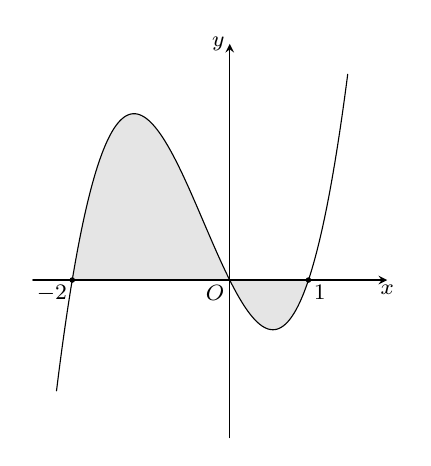
\begin{tikzpicture}[scale=1,font=\footnotesize,line join=round,line cap=round,>=stealth]
		\fill[gray!20,smooth]  (-2,0)--plot[domain=-2:1] (\x,{(\x+2)*(\x)*(\x-1)})
			--  (1,0) -- cycle;
		\draw[->]  (-2.5,0)--(2,0) node[below] {$x$};
		\draw[->] (0,-2)--(0,3)  node[left] {$y$};
		\draw (0,0) node [below left]  {$O$};
		\fill (-2,0) circle (1pt) node[below left]{$-2$} 
			 (1,0) circle (1pt) node[below right]{$1$};
		\draw[smooth,samples=200] plot[domain=-2.2:1.5] (\x,{(\x+2)*(\x)*(\x-1)}); 
	\end{tikzpicture}}
	\shortans{4} 
	\loigiai{ 
		Ta có diện tích phần hình phẳng gạch chéo trong hình bằng 
		 \allowdisplaybreaks
		\begin{eqnarray*}
			\displaystyle\int_{-2}^1 |f(x)| \mathrm{\,d}x&=&\int_{-2}^0 |f(x)| \mathrm{\,d}x+\int_{0}^1 |f(x)| \mathrm{\,d}x=\int_{-2}^0 f(x) \mathrm{\,d}x-\int_{0}^1 f(x) \mathrm{\,d}x\\ 
			&=&3-(-1)=4. 
		\end{eqnarray*}
	} 
\end{bt}

% nguồn: Phan2_Lop_12_Dai_so_Chuong_4
\begin{bt}%[2D4H3-1]%[ma:5c0c3149]
	Cho $(H)$ là hình phẳng được tô đậm trong hình vẽ và được giới hạn bởi các đường có phương trình $y=\dfrac{10}{3}x-x^2$, $y=\begin{cases} -x & \text{ khi } x \le 1 \\ x-2 & \text{ khi } x>1
\end{cases}$. Diện tích của $(H)$ bằng bao nhiêu?
 \shortans{6,5}
\loigiai{ 
	Ta tìm giao điểm của parabol $y=\dfrac{10}{3}x-x^2$ với hai nhánh của hàm số còn lại. 
	\begin{itemize}
		\item Với $x \le 1$: $\dfrac{10}{3}x-x^2 = -x \Leftrightarrow  x^2-\dfrac{13}{3}x=0 \Leftrightarrow x(x-\dfrac{13}{3})=0$.
		Ta nhận nghiệm $x=0$ (thỏa  mãn $x \le 1$).
		\item Với $x  > 1$: $\dfrac{10}{3}x-x^2 = x-2 \Leftrightarrow x^2-\dfrac{7}{3}x-2=0 \Leftrightarrow 3x^2-7x-6=0$.
		Phương trình có hai nghiệm $x=3$ và $x=-\dfrac{2}{3}$. Ta nhận nghiệm $x=3$ (thỏa mãn  $x>1$).
	\end{itemize}
	Vậy hình phẳng $(H)$ được giới  hạn bởi hai đồ thị trên đoạn $[0,3]$.\\
	 Diện tích hình phẳng $(H)$ là
	\begin{align*}
		S &=  \int_{0}^{1} \left| \left(\frac{10}{3}x-x^2\right) - (-x) \right|\mathrm{d}x + \int_{1}^{3} \left| \left(\frac{10}{3}x-x^2\right) - (x-2) \right|\mathrm{d}x \\
		&= \int_{0}^{1} \left(\frac{13}{3}x - x^2\right)\mathrm{d}x + \int_{1}^{3} \left(-\frac{7}{3}x - x^2  + 2\right)\mathrm{d}x\\
		&= \dfrac{11}{6} + \dfrac{45}{6}  - \dfrac{17}{6} = \frac{13}{2}.
	\end{align*}
	Vậy, diện tích của $(H)$ bằng \textbf{$\dfrac{13}{2}$}. 
 }
\end{bt}

% nguồn: Phan2_Lop_12_Dai_so_Chuong_4
\begin{bt}%[2D4H3-1]%[ma:908d5841]
	Cho hàm số $ f(x) = \begin{cases} 7-4x^3 & \text{ khi } 0 \le x \le 1 \\ 4-x^2 & \text{ khi } x > 1
\end{cases} $. Tính diện tích hình phẳng giới hạn bởi đồ thị hàm số $f(x)$ và các đường thẳng $x=0, x=3, y=0$.
\shortans{10} 
 \loigiai{
	Diện tích  $S$ của hình phẳng cần tìm
	\begin{align*}
		 S &= \int_{0}^{1} |7-4x^3|\mathrm{d}x + \int_{1}^{3} |4-x^2|\mathrm{d}x \\
		&= \int_{0}^{1} (7-4x^3)\mathrm{d}x + \int_{1}^{2} (4-x^2)\mathrm{d}x - \int_{2}^{3} (4-x^2)\mathrm{d}x  \\
		&=6 + \frac{5}{3} + \frac{7}{3} = 6 +  \frac{12}{3} = 6+4 = 10.
	\end{align*}
	Vậy, diện tích hình phẳng cần tìm là \textbf{10}. 
 }
\end{bt}

% nguồn: Phan2_Lop_12_Dai_so_Chuong_4
\begin{bt}%[2D4H3-1]%[ma:4c9d23cf]
	\immini{Một hoa  văn được tạo từ một miếng bìa mỏng hình chữ nhật bằng cách vẽ hai phần bằng nhau có hình dạng parabol như hình bên. Biết rằng $AB=4$ (dm); $BC=8$ (dm), giá trang trí $1$ (dm$^2$) hoa văn được tô đậm là $60\,000$ đồng và $1$ (dm$^2$) phần trắng là $45\,000$ đồng, cần bỏ ra bao nhiêu triệu đồng để trang trí $100$ hoa văn đó?}{
	\begin{tikzpicture}[scale=1,font=\footnotesize,line join=round,line cap=round,>=stealth]
			\begin{scope}
				 \draw (-2,-1) rectangle (2,1);
				\draw[samples=200,domain=-2:2,smooth,variable=\x] plot (\x,{(1/4)*(\x)^2+0*(\x)}); 
				\draw[samples=200,domain=-2:2,smooth,variable=\x] plot (\x,{-(1/4)*(\x)^2+0*(\x)}); 
				\draw[dashed,thin,pattern=north east lines]plot[samples=200,domain=-2:2,smooth,variable=\x] (\x,{(1/4)*(\x)^2})--(2,1); 
				 \draw[dashed,thin,pattern=north east lines]plot[samples=200,domain=-2:2,smooth,variable=\x] (\x,{-(1/4)*(\x)^2})--(2,-1);
			\end{scope}
			\node at  (-2,1) [above left]{$A$};
			\node at (2,-1) [below right]{$C$}; 
			\node at (-2,-1) [below left]{$B$}; 
		\end{tikzpicture}
	 }
	\shortans{160} 
	 \loigiai{
		Vì $AB=4$ (dm); $BC=8$ (dm) $\Rightarrow A(-2;4)$, $B(2;4)$ $C(2;-4)$, $D(-2;-4)$, parabol có đỉnh $O(0;0)$ nên có công thức  là $y=x^2$ hoặc $y=-x^2$.
		\begin{center}
			\begin{tikzpicture}[scale=1,font=\footnotesize,line join=round,line cap=round,>=stealth]
					\draw[->] (-2.2,0)--(2.2,0) node[below right] {$x$}; 
					\draw[->] (0,-1.1)--(0,1.6) node[below left]  {$y$};
					\draw  (0,0) node [below left] {$O$};
					\begin{scope}
						\draw (-2,-1) rectangle  (2,1);
						\draw[samples=200,domain=-2:2,smooth,variable=\x] plot (\x,{(1/4)*(\x)^2+0*(\x)}); 
						\draw[samples=200,domain=-2:2,smooth,variable=\x]  plot (\x,{-(1/4)*(\x)^2+0*(\x)});
						\draw[dashed,thin,pattern=north east lines]plot[samples=200,domain=-2:2,smooth,variable=\x]  (\x,{(1/4)*(\x)^2})--(2,1);
						 \draw[dashed,thin,pattern=north east lines]plot[samples=200,domain=-2:2,smooth,variable=\x] (\x,{-(1/4)*(\x)^2})--(2,-1);
					\end{scope}
					 \node at (-2,1) [above left]{$A$};
					\node at (2,-1) [below  right]{$C$};
					\node at  (-2,-1) [below left]{$B$};
					 \node at (2,1) [above right]{$D$};
				\end{tikzpicture}
		\end{center}
		Diện tích phần được tô đậm là $S_1=4\displaystyle \int_0^2 x^2 \mathrm{\,d}x=\dfrac{32}{3}$ (dm$^2$).\\ 
		Diện tích hình  chữ nhật là $S=4\cdot 8=32$ (dm$^2$).\\
		Diện tích phần  trắng là $S_2=S-S_1=32-\dfrac{32}{3}=\dfrac{64}{3}$ (dm$^2$).\\
		Số tiền cần bỏ ra để trang trí $100$  hoa văn là
		$$T=\left(\dfrac{32}{3}\cdot 60\,000+\dfrac{64}{3}\cdot 45\,000\right)\cdot  100=160\,000\,000\text{ (đồng)}.$$
	 }
\end{bt}

% nguồn: Phan2_Lop_12_Dai_so_Chuong_4
\begin{bt}%[2D4H3-1]%[ma:98ff268c]
	Hình phẳng giới hạn bởi trục tung, đường thẳng  $y=-8$ và đồ thị hàm số $y=x^3$ có diện tích là bao nhiêu?
	 \shortans{12}
	 \loigiai{
		Ta có $S=\displaystyle\int_{-2}^0\left|x^3-(-8)\right|  \mathrm{\,d}x=\displaystyle\int_{-2}^0\left(x^3+8\right) \mathrm{\,d}x=\left.\left(\dfrac{x^4}{4}+8 x\right)\right|_{-2}^0=12$.
	} 
\end{bt}

% nguồn: Phan2_Lop_12_Dai_so_Chuong_4
\begin{bt}%[2D4H3-1]%[ma:7a84c92b]
	Diện tích hình phẳng giới hạn bởi hai đồ thị hàm số $y=\dfrac{x^2-2x+3}{x-1}$,  $y=x$ và hai đường thẳng $x=2$, $x=3$ bằng $S=a\ln 2 + b$. Giá trị của $a+b$ bằng bao nhiêu?
	 \shortans{1}
	\loigiai{ 
		Diện  tích $S$ của hình phẳng được tính bằng tích phân:
		$$ S = \int_{2}^{3} \left|  \frac{x^2-2x+3}{x-1} - x \right| \mathrm{d}x .$$
		Ta  có
		$$ \frac{x^2-2x+3}{x-1} - x = \frac{x^2-2x+3 - x(x-1)}{x-1} = \frac{x^2-2x+3 - x^2+x}{x-1} =  \frac{-x+3}{x-1} .$$
		Vì $\dfrac{-x+3}{x-1} \ge 0$ với  mọi $x \in [2{,}3]$. \\
		 Do đó
		$$ S =\int_{2}^{3} \left(\frac{-x+3}{x-1}\right) \mathrm{d}x = \int_{2}^{3} \left(-1 + \frac{2}{x-1}\right) \mathrm{d}x = 2\ln 2 -  1. $$
		Theo đề bài, $S = a\ln  2 + b$. So sánh với kết quả vừa tìm được, ta có $ a=2 \quad \text{ và} \quad b=-1 .$\\
		Vậy, giá trị của $a+b$  là $1$.
	 }
\end{bt}

% nguồn: Phan2_Lop_12_Dai_so_Chuong_4
\begin{bt}%[2D4H3-1]%[ma:e2e9ec1b]
	Tìm $a$ để diện tích $S$ của hình phẳng giới hạn bởi  $(P): y=\dfrac{x^2-2x}{x-1}$, đường thẳng $d:y=x-1$ và $x=a, x=2a$ ($a>1$) bằng $\ln 3$?
	\shortans{2} 
	 \loigiai{
		Diện tích $S$  của hình phẳng được tính bằng tích phân
		$$ S = \int_{a}^{2a} \left| \frac{x^2-2x}{x-1} - (x-1) \right| \mathrm{d}x .$$ 
		 Ta có
		$$ \frac{x^2-2x}{x-1} - (x-1) = \frac{x^2-2x - (x-1)^2}{x-1} = \frac{x^2-2x - (x^2-2x+1)}{x-1} =  \frac{-1}{x-1} .$$
		Do $a>1$ nên với mọi $x \in [a, 2a]$, ta có $x-1 > 0$, suy ra $\dfrac{-1}{x-1} <  0$.
		Do đó 
		$  \left| \dfrac{-1}{x-1} \right| = \dfrac{1}{x-1} .$
		 Vậy
		$$ S  = \int_{a}^{2a} \frac{1}{x-1} \mathrm{d}x = \ln\left(\frac{2a-1}{a-1}\right). $$
		Theo đề bài, $S = \ln 3$, nên 
		\begin{align*}
			 \ln\left(\frac{2a-1}{a-1}\right) = \ln 3 & \Leftrightarrow 2a-1 = 3(a-1) = 3a-3 \\ & \Leftrightarrow 2a-1 = 3(a-1) = 3a-3\Leftrightarrow a=2.
		\end{align*}
		Vậy, giá trị cần tìm  là \textbf{$a=2$}.
	} 
\end{bt}

% nguồn: Phan2_Lop_12_Dai_so_Chuong_4
\begin{bt}%[2D4H3-1]%[ma:5aae6f6c]
	\immini{Cho đồ thị hàm số $y=\cos x$ và hình phẳng được gạch sọc như bên. Tính diện tích hình phẳng đó (viết kết quả dưới dạng số thập phân và làm tròn đến  hàng phần mười).}
	{\begin{tikzpicture}[line join=round,line cap=round,>=stealth]
		\begin{scope}
			\clip  (-0.7,-1.2) rectangle (4,3.5);
			 \draw[samples=100,domain=-0.5:4,smooth,variable=\x] plot (\x,{(\x)});
			\draw[samples=100,domain=-0.7:4,smooth,variable=\x] plot (\x,{cos ((\x)  r)});
			\fill[pattern=north east lines]  plot[domain=1:3] (\x,{cos ((\x) r)})--(1,0.5403)--(1,1)--(3,3)--(3,-1)--cycle;
		\end{scope}
		\draw[->] (-0.8,0)--(4.1,0) node[below  left] {$x$};
		\draw[->] (0,-1.3)--(0,4) node[below  left] {$y$};
		\draw (0,0) node [above left]  {$O$};
		\foreach \x/\nx  in {1/1}
		\draw[thin] (\x,1pt)--(\x,-1pt) node [below]  {$\nx$};
		 \foreach \x/\nx in {3/3}
		\draw[thin] (\x,1pt)--(\x,-1pt) node  [below right] {$\nx$};
		\foreach \y/\ny in  {-1/-1,1/1}
		\draw[thin]  (1pt,\y)--(-1pt,\y) node [above left] {$\ny$}
			(3,-1)--(3,3); 
		\draw[dashed,thin](1,0)--(1,1)--(0,1); 
		\draw (2.1,-1) node[rotate=-40]{$y=\cos x$}; 
		\draw (2,2.5)  node[rotate=45]{$y=x$};
	\end{tikzpicture}}
	 \shortans{4,7}
	 \loigiai{
		Hình phẳng đã cho giới hạn bởi đồ thị của  các hàm số $y=\cos x$, $y=x$ và hai đường thẳng $x=1$, $x=3$.\\
		Khi đó, diện  tích hình phẳng là $S=\displaystyle\int_1^3 |\cos x-x| \mathrm{\,d} x$.\\
		Vì $x\ge\cos x$, $\forall x\in[1;3]$ nên  ta có\\
		$S=\displaystyle\int_1^3 (x-\cos x) \mathrm{\,d} x=\left.\left(\dfrac{x^2}{2}-\sin x\right)\right|_1 ^3=4-\sin 3+\sin 1  \approx 4{,}7.$
	} 
\end{bt}

% nguồn: Phan2_Lop_12_Dai_so_Chuong_4
\begin{bt}%[2D4H3-1]%[ma:e544d611]
	Cho hàm số $y=f(x)$. Đồ thị hàm số $y=f'(x)$ là đường cong trong hình dưới. Biết rằng diện tích  của các phần hình phẳng $A$ và $B$ lần lượt là $S_A=4$ và $S_B=10$. Tính giá trị của $f(3)$, biết giá trị của $f(0)=2$.
	\begin{center}
		\begin{tikzpicture}[scale=1.2,>=stealth,font=\footnotesize,line join=round,line cap=round]
				 \def\a{3} \def\b{-8.4} \def\c{4.8} \def\d{0}
				\def\xmin{-1}  \def\xmax{2.5}
				\def\ymin{-2}  \def\ymax{1.5}
				\draw[->]  (\xmin,0)--(\xmax,0) node [below]{$x$};
				\draw[->] (0,\ymin)--(0,\ymax)  node [left]{$y$};
				\node at (0,0) [below  left]{$O$};
				\draw[smooth,samples=300,domain=-0.25:2.15]  plot (\x,{\a*(\x)^3+\b*(\x)^2+\c*(\x)+\d}) node[left]{$y=f'(x)$};
				\fill[pattern=north east  lines,opacity=0.6] plot[domain=0:0.8](\x,{\a*(\x)^3+\b*(\x)^2+\c*(\x)+\d})--cycle;
				\fill[pattern=north  east lines,opacity=0.6] plot[domain=0.8:2](\x,{\a*(\x)^3+\b*(\x)^2+\c*(\x)+\d})--cycle;
				\node at (0.4,0.3){$S_1$}; 
				\node at  (1.45,-0.6){$S_2$};
				\node at (2,0)[below  right]{$3$};
				\node at (1,0)[below  left]{$1$};
				\fill (0,0)  circle (0.04)
					 (2,0) circle (0.04);
			\end{tikzpicture}
	\end{center}
	 \shortans{-4}
	 \loigiai{
		Dựa vào đồ thị của $y=f'(x)$ và  định nghĩa của tích phân xác định, ta có thể liên hệ diện tích và tích phân như sau
		\begin{itemize}
			\item Trên đoạn $[0, 1]$, đồ thị $f'(x)$ nằm phía trên trục hoành, do  đó
			$$ \int_{0}^{1} f'(x)\mathrm{d}x = S_A = 4 \Rightarrow f(1)=S_A+f(0)=4+2=6.$$ 
			\item Trên đoạn $[1, 3]$, đồ thị  $f'(x)$ nằm phía dưới trục hoành, do đó
			 $$ \int_{1}^{3} f'(x)\mathrm{d}x = -S_B = -10 \Rightarrow f(3)=f(1)-S_B=-4.$$
		\end{itemize}
	Vậy $ f(3) = f(0) - 6 = 2  - 6 = -4 $.}
\end{bt}

% nguồn: Phan2_Lop_12_Dai_so_Chuong_4
\begin{bt}%[2D4V3-1]%[ma:86a29934]
	\immini[thm]{Hình vẽ dưới đây cho biết một miền $D$ (được tô đậm) nằm trong hình vuông cạnh  bằng $4$, miền $D$ này gồm những điểm có khoảng cách tới tâm hình vuông nhỏ hơn hoặc bằng khoảng cách tới cạnh gần nhất của hình vuông.
	Tính diện tích miền $D$, với kết quả làm tròn đến chữ số  thập phân thứ nhất.}
	{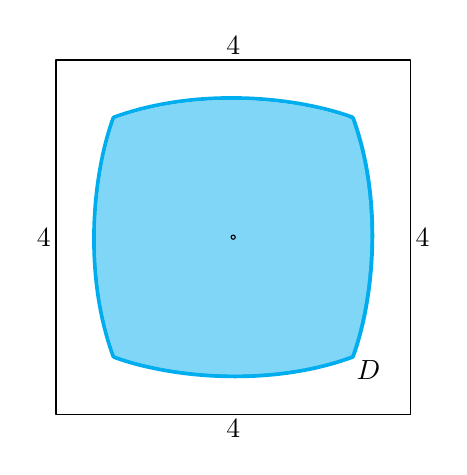
\begin{tikzpicture}[scale=.75,line cap=round,line join=round]
		\def\c{(-2,2)..controls++(20:1.48) and++(160:1.01)..(2,2)} 
		\def\d{(0,0)--(-2,2)..controls++(20:1.48)  and++(160:1.01)..(2,2)--cycle}
		\foreach \x in{0,1,2,3}{ 
			\begin{scope}[rotate=90*\x]
			\draw[line width=1mm,cyan] \c; 
			\end{scope}
			\foreach \x in{0,1,2,3}{ 
			\begin{scope}[rotate=90*\x]
			\fill[cyan!50] \d; 
			\end{scope}}
		} 
		 \draw (3,3)--(3,-3)--(-3,-3)--(-3,3)--cycle;
		\draw (0,0) circle (1pt); 
		 \node[below right] at (2,-2) {$D$};
		\foreach \x/\y in{(3,0)/right,(0,3)/above,(-3,0)/left,(0,-3)/below}{\node[\y] at  \x {$4$};}
	\end{tikzpicture}}
	 \shortans{3,5}
	\loigiai{ 
		Từ định nghĩa \lq\lq tập hợp các điểm cách đều $1$ điểm và $1$ đường thẳng (điểm không thuộc đường thẳng) là một đường parabol\rq\rq, ta suy ra miền $D$ được giới hạn bởi $4$  đường parabol có tiêu điểm là tâm hình vuông và đường chuẩn là cạnh của hình vuông.
		\begin{center}
			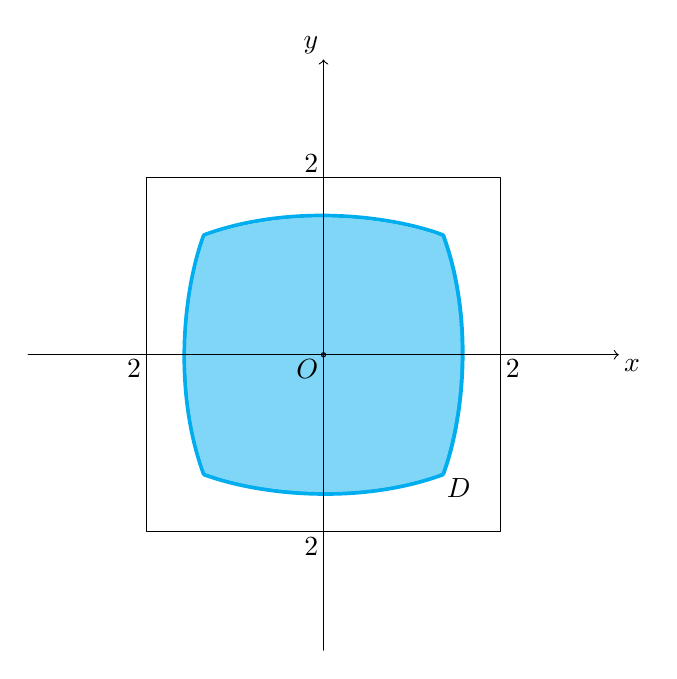
\begin{tikzpicture}[scale=.75,line cap=round,line join=round]
					 \def\c{(-2,2)..controls++(20:1.48) and++(160:1.01)..(2,2)}
					 \def\d{(0,0)--(-2,2)..controls++(20:1.48) and++(160:1.01)..(2,2)--cycle}
					\foreach \x in{0,1,2,3}{ 
						\begin{scope}[rotate=90*\x]
						 \draw[line width=1mm,cyan] \c;
						\end{scope}
						\foreach \x in{0,1,2,3}{ 
						\begin{scope}[rotate=90*\x]
						 \fill[cyan!50] \d;
						\end{scope}}
					} 
					\draw[->] (-5,0)--(0,0) node[below left]{$O$}--(5,0) node[below  right]{$x$};
					\draw[->] (0,-5)--(0,5) node[above left]{$y$}; 
					\draw (3,3)--(3,-3)--(-3,-3)--(-3,3)--cycle; 
					\draw (0,0) circle (1pt); 
					 \node[below right] at (2,-2) {$D$};
					\foreach \x/\y  in{(3,0)/below right,(0,3)/above left,(-3,0)/below left,(0,-3)/below left}{\node[\y] at \x {$2$};}
				\end{tikzpicture}
		\end{center}
		Dựng  hệ toạ độ như hình vẽ, tìm phương trình các đường parabol rồi dựa vào ứng dụng của tích phân tính được diện tích miền $D$ là \[S=4\left[\displaystyle\int_0^{2\sqrt{2}-2}\left(-\dfrac{1}{4} x^2+1\right) \mathrm{\,d}x+\displaystyle\int_{2\sqrt{2}-2}^1(2\sqrt{1-x}) \mathrm{\,d}x\right]=\dfrac{64\sqrt{2}-80}{3} \approx 3{,}5.\]
	} 
\end{bt}

% nguồn: Phan2_Lop_12_Dai_so_Chuong_4
\begin{bt}%[2D4V3-1]%[ma:14d801f7]
	Một nhóm các kỹ sư muốn xây dựng một cây cầu vòm dàn thép với giá đỡ  dưới bằng thép cao cấp có hình dáng là một đường cong Parabol nối từ $2$ cột trụ A và B nằm bên dưới cây cầu, biết hai cột trụ cách nhau $400$ m, khoảng cách từ trụ A đến cây cầu là $50$ m và AB song song với mặt đường.
	Gắn hệ trục tọa độ Oxy vào cây cầu với đơn vị trục tọa độ là $10$ m. Giá đỡ  dưới bằng thép là đường cong Parabol tạo với $2$ trục tọa độ các hình phẳng có diện tích $S_1$, $S_2$ như hình vẽ bên, biết rằng
	 $$
	S_2  - 2S_1 = \dfrac{2\,200}{21}.
	$$ 
	Điểm cao nhất của giá đỡ dưới bằng thép cao cấp cách mặt  đường cây cầu bao~nhiêu mét (làm tròn đến hàng phần mười).
	\begin{center}
		\begin{tikzpicture}[line join=round,line cap=round,>=stealth]
				\draw[->] (-1,0) -- (9,0)  node[right] {$x$};
				 \draw[->] (0,-3) -- (0,2.5) node[above] {$y$};
				\fill (0,0) circle (1pt) node[below left]{$O$}; 
				\fill  (0,-1) circle (1pt) node[left]{$-5$};
				\fill (0,-1)  circle (1pt) node[below right]{$A$};
				\fill (6.54,-1) circle (1pt) node[below]{$B$}; 
				\node at (3.25,.7)  {$S_2$};
				\node at (0.24,-.35) {$S_1$}; 
				\draw[dashed,<->] (0,-1) -- (6.54,-1) node[midway,above]{$40$}; 
				\draw[dashed] (6.54,-1)  -- (6.54,0);
				\draw[domain=-1:7.5,smooth] plot (\x,{(-0.19)*(\x)^2 + 1.25*(\x) - 1}); 
			\end{tikzpicture}
	\end{center}
	 \shortans{64,3}
	 \loigiai{
		\begin{center}
			\begin{tikzpicture}[line join=round,line cap=round,>=stealth]
					\draw[->] (-1,0) -- (9,0)  node[right] {$x$};
					\draw[->] (0,-3) -- (0,2.5) node[above] {$y$}; 
					\fill (0,0) circle (1pt) node[below  left]{$O$};
					\fill (0,-1) circle (1pt)  node[left]{$-5$};
					\fill (0,-1) circle (1pt) node[below  right]{$A$};
					\fill (6.54,-1) circle  (1pt) node[below]{$B$};
					 \fill (6.54,0) circle (1pt) node[above]{$C$};
					\node at  (3.25,.7) {$S_2$};
					\node  at (3.25,-.35) {$S_3$};
					 \node at (0.24,-.35) {$S_1$};
					\node at  (6.25,-.35) {$S_1$};
					 \draw[dashed,<->] (0,-1) -- (6.54,-1) node[midway,above]{$40$};
					\draw[dashed] (6.54,-1) --  (6.54,0);
					\draw[domain=-1:7.5,smooth] plot (\x,{(-0.19)*(\x)^2 +  1.25*(\x) - 1});
				\end{tikzpicture}
		\end{center}
		Parabol là $y = f(x) = ax^2 + bx + c \quad (a \neq 0)$.\\ 
		Parabol đi qua $(0; -5)$, $(40; -5)$ nên 
		\begin{itemize}
			\item $f(0) = -5 \Rightarrow c = -5.  \quad (1)$
			\item $f(40)  = -5 \Rightarrow 1\,600a + 40b + c = -5. \quad (2)$
		\end{itemize}
		Ta có 
		\begin{eqnarray*}
			S_2 - 2S_1 &=& S_2  - (S_{OABC} - S_3)\\
			&=&  S_2 - S_{OABC} + S_3\\
			&=& (S_2  + S_3) - S_{OABC}\\
			&=& \displaystyle\int_{0}^{40} (ax^2 + bx  + c + 5) \,\mathrm{d}x -5\cdot40\\
			&=& \left( a \cdot \dfrac{x^3}{3} + b \cdot \dfrac{x^2}{2} + (c+5)  x \right) \Bigg|_0^{40} - 200\\
			&=&  \left( a \cdot \dfrac{40^3}{3} + b \cdot \dfrac{40^2}{2} + (c+5) \cdot 40 \right) - 200\\
			&=& \dfrac{40^3}{3} a +  \dfrac{40^2}{2} b + 40c - 200.
		\end{eqnarray*}
		 Từ giả thiết suy ra
		$$ 
		\dfrac{40^3}{3} a + \dfrac{40^2}{2} b + 40c  = \dfrac{2\,200}{21}. \quad (3)
		 $$
		Từ (1), (2) và (3)  suy ra
		$$ 
		a = \dfrac{-1}{35}, \quad b = \dfrac{8}{7}, \quad  c = -5
		 $$
		Vậy parabol $y  = \dfrac{-1}{35} x^2 + \dfrac{8}{7} x - 5$.\\
		 Hoành độ của đỉnh parabol là $x_t = \dfrac{-b}{2a} = \dfrac{-\dfrac{8}{7}}{2 \cdot \left(\dfrac{-1}{35}\right)} = 20$.\\
		Tung độ của đỉnh parabol là $y_I=-\dfrac{1}{35} \cdot 20^2+\dfrac{8}{7} \cdot 20-5=\dfrac{45}{7}$.\\ 
		Điểm cao nhất của giá đỡ dưới bằng thép cao cấp cách măt  đường cây cầu là $10 \cdot \dfrac{45}{7} \approx 64{,}3`(\mathrm{m})$.
	 }
\end{bt}

% nguồn: Phan2_Lop_12_Dai_so_Chuong_4
\begin{bt}%[2D4V3-1]%[ma:e78cd642]
	Một viên đạn được bắn lên từ mặt đất theo phương thẳng đứng với vận tốc ban đầu  $29{,}4 \mathrm{~m} / \mathrm{s}$. Quãng đường viên đạn đi được từ lúc bắn lên cho tới khi chạm đất là bao nhiêu mét? Biết gia tốc trọng trường là $9{,}8\ \mathrm{m} / \mathrm{s}^2$.
	\shortans{88,2} 
	\loigiai{ 
		 \allowdisplaybreaks
		\begin{eqnarray*}
			 && v=29{,}4-9{,}8 t;\\
			&& v=0 \Leftrightarrow 29{,}4-9{,}8 t=0  \Leftrightarrow t=3; \\
			&& S=2 \displaystyle\int_0^3(29{,}4-9{,}8 t) \mathrm{\,d}t=\left.2\left(29{,}4 t-4{,}9 t^2\right)\right|_0^3=88{,}2\  (\mathrm{m}).
		\end{eqnarray*}
	} 
\end{bt}

% nguồn: Phan2_Lop_12_Dai_so_Chuong_4
\begin{bt}%[2D4V3-1]%[ma:c91996c9]
	Người ta thiết kế một mẫu gạch lát nền nhà có dạng hình vuông cạnh $4$ dm. Bốn góc viên gạch màu trắng, phần ở giữa màu xanh (Hình 5). Đường viền của phần màu xanh bao gồm bốn đoạn thẳng nằm  trên các cạnh hình vuông và bốn đường cong có tính chất: Tích khoảng cách từ một điểm bất kì thuộc đường cong đó đến hai trục đối xứng của viên gạch (hai đường thẳng đi qua tâm viên gạch và lần lượt song song với hai cạnh vuông góc) bằng $2$ dm$^2$.
	Hãy cho biết phần màu xanh có diện  tích bằng bao~nhiêu decimét vuông (làm tròn kết quả đến hàng phần mười)?
	\shortans{13,5} 
	\begin{center}
		\begin{tikzpicture}[line join=round,line cap=round,>=stealth,font=\scriptsize]
				\tikzset{every node/.style={scale=0.9}} 
				 \fill[gray] (0,0)--(0,2)--plot[domain=1:2] (\x,{(0*(\x)+2)/(1*(\x)+0)})--(2,0)--(2,1)--plot[domain=2:1] (\x,{(0*(\x)+-2)/(1*(\x)+0)})--(1,-2)--(0,-2)--cycle;
				\fill[xscale=-1,gray]  (0,0)--(0,2)--plot[domain=1:2] (\x,{(0*(\x)+2)/(1*(\x)+0)})--(2,0)--(2,1)--plot[domain=2:1] (\x,{(0*(\x)+-2)/(1*(\x)+0)})--(1,-2)--(0,-2)--cycle;
				\draw (-2,-2) rectangle (2,2); 
			\end{tikzpicture}
	\end{center}
	 \loigiai{
		Gắn trục toạ độ $Oxy$ vào viên gạch sao cho hai trục trùng với hai đường đối xứng, gốc $O$ ở tâm hình vuông như hình  dưới. Giả sử toạ độ một điểm trên đường viền cong là $( x;y)$. \\
		 Theo giả thiết, ta có $| xy |=2$. Suy ra $ y=\dfrac {2}{x}$ hoặc $ y=-\dfrac {2}{x}$.\\ Ứng với hình dưới, ta có các đường viền cong $AK$, $DE$ là một phần của đồ thị hàm số $ y=-\dfrac {2}{x}$; các đường viền cong $BC,GH$ là một phần của đồ thị hàm số $ y=\dfrac {2}{x}$.\\
		\begin{center}
			\begin{tikzpicture}[line join=round,line cap=round,>=stealth,font=\scriptsize]
					\tikzset{every node/.style={scale=0.9}} 
					 \path (-1,2) coordinate (A)
						 (1,2) coordinate (B)
						 (2,1) coordinate (C)
						(2,-1) coordinate (D) 
						(1,-2) coordinate (E) 
						(-1,-2)  coordinate (G)
						(-2,-1)  coordinate (H)
						(-2,1)  coordinate (K);
					\fill[gray] (0,0)--(0,2)--plot[domain=1:2]  (\x,{(0*(\x)+2)/(1*(\x)+0)})--(2,0)--(2,1)--plot[domain=2:1] (\x,{(0*(\x)+-2)/(1*(\x)+0)})--(1,-2)--(0,-2)--cycle;
					\fill[xscale=-1,gray] (0,0)--(0,2)--plot[domain=1:2] (\x,{(0*(\x)+2)/(1*(\x)+0)})--(2,0)--(2,1)--plot[domain=2:1] (\x,{(0*(\x)+-2)/(1*(\x)+0)})--(1,-2)--(0,-2)--cycle; 
					\draw[->] (-3.1,0)--(3.1,0) node[below left] {$x$}; 
					\draw[->] (0,-3.1)--(0,3.1)  node[below left] {$y$};
					\draw (0,0) node  [above left] {$O$};
					 \foreach \x/\nx in {-2/-2,-1/-1,1/1,2/2}
					\draw[thin] (\x,1pt)--(\x,-1pt) node [shift={(-60:0.3)}] {$\nx$}; 
					 \foreach \y/\ny in {-2/-2,-1/-1,2/2}
					\draw[thin] (1pt,\y)--(-1pt,\y) node [shift={(145:0.3)}]  {$\ny$};
					\draw[dashed,thin]  (A)--(G)
						(B)--(E) 
						(C)--(K) 
						(D)--(H); 
					\begin{scope}
						\clip  (-2,-2) rectangle (2,2);
						\draw[samples=100,domain=-2:-0.01,smooth,variable=\x] plot  (\x,{(0*(\x)+2)/(1*(\x)+0)});
						\draw[samples=100,domain=0.01:2,smooth,variable=\x] plot  (\x,{(0*(\x)+2)/(1*(\x)+0)});
						\draw[dashed,thin] (-2,0/1)--(2,0/1); 
						\draw[samples=100,domain=-2:-0.01,smooth,variable=\x]  plot (\x,{(0*(\x)+-2)/(1*(\x)+0)});
						 \draw[samples=100,domain=0.01:2,smooth,variable=\x] plot (\x,{(0*(\x)+-2)/(1*(\x)+0)});
						\draw[dashed,thin] (-2,0/1)--(2,0/1); 
					\end{scope}
					\draw (-2,-2)  rectangle (2,2);
					\foreach \t/\g in  {A/90,B/90,C/0,D/0,E/-90,G/-90,H/180,K/180}{
						\path (\t) node[shift={(\g:9pt)},font=\scriptsize]{$ \t $}; 
					 }
				\end{tikzpicture}
		\end{center}
		Khi đó, diện tích phần màu xanh bằng 
		\allowdisplaybreaks 
		\begin{eqnarray*}
			& &\displaystyle\int_{-2}^{-1} \left| -\dfrac {2}{x}-\dfrac {2}{x} \right|\mathrm{\,d}x +\displaystyle\int_1^2  \left| \dfrac {2}{x}-\dfrac {-2}{x} \right|\mathrm{\,d}x +S_{ABEG}\\
			&=&\displaystyle\int_{-2}^{-1} \left( -\dfrac {2}{x}-\dfrac {2}{x} \right)\mathrm{\,d}x  +\displaystyle\int_1^2 \left( \dfrac {2}{x}-\dfrac {-2}{x} \right)\mathrm{\,d}x +4{,}2\\
			&=&\left.-4\ln |x|\right|_{-2}^{-1} + \left.4\ln |x|\right|_1^2+8\approx 13{,}5 \,(\text{dm}^2). 
		\end{eqnarray*}
	 }
\end{bt}

% nguồn: Phan2_Lop_12_Dai_so_Chuong_4
\begin{bt}%[2D4V3-1]%[ma:0820c297]
	Một ô tô đang chạy với vận tốc $18 \mathrm{~m} / \mathrm{s}$ thì người  lái hãm phanh. Sau khi hãm phanh, ô tô chuyển động chậm dần đều với vận tốc $v(t)=-36 t+18\ (\mathrm{m} / \mathrm{s})$ trong đó $t$ là khoảng thời gian tính bằng giây kể từ lúc bắt đầu hãm phanh. Hỏi từ lúc hãm phanh đến khi dừng hẳn, ô tô còn di chuyển bao nhiêu mét?
	\shortans{45} 
	 \loigiai{
		Lấy mốc thời gian là lúc ô tô  bắt đầu hãm phanh.\\
		Gọi $T$ là thời điểm ô tô dừng.\\ Ta có $v(T)=0$ suy ra $-36 \mathrm{~T}+18=0  \Rightarrow T=0{,}5$ (s).\\
		Khoảng thời gian từ lúc hãm phanh đến lúc ô tô dừng hẳn là $0{,}5 \mathrm{~s}$. Trong  khoảng thời gian đó, ô tô di chuyển được quãng đường là
		\[S=\displaystyle\int_0^{0{,}5}(-36 t+18)\ \mathrm{\,d}t=\left.\left(-18 t^2+18  t\right)\right|_0^{0{,}5}=4{,}5\ (\mathrm{m}). \]
	 }
\end{bt}

% nguồn: Phan2_Lop_12_Dai_so_Chuong_4
\begin{bt}%[2D4V3-1]%[ma:89b52acd]
	 \immini[thm]{
	Một bức tường hình chữ nhật $ABCO$ cao $4$ m, dài $8$ m. Bạn Bình trang trí bức tường bằng cách vẽ đường cong là một hàm số  bậc ba $y=\dfrac{1}{35}x(x-2)(x-8)+2$ trong hệ trục tọa độ như hình bên dưới, mỗi phần sơn một màu, phần phía trên sơn màu xanh da trời và phần phía dưới sơn màu trắng.
	Biết 1 hộp sơn sơn được $4 \mathrm{m}^2$. Bạn  Bình phải mua tối thiểu $m$ hộp sơn màu xanh và $n$ hộp sơn màu trắng để sơn bức tường. Hãy tính $m-n$.
	 \shortans{3}
	 }{
	\begin{tikzpicture}[line join=round,line cap=round,>=stealth,scale=0.7]
			 \tikzset{label style/.style={font=\footnotesize}}
			\fill[cyan] (0,2)--plot[samples=200,domain=-1:8,smooth,variable=\x] (\x,{1/35*(\x)^3-10/35*(\x)^2+16/35*(\x)+2})--(8,4)--(0,4)--cycle; 
			 \draw[->] (-1,0)--(10,0) node[below right] {$x$};
			\draw[->] (0,-1)--(0,5) node[above  left] {$y$};
			\draw (0,0) node [below  left] {$O$};
			 \foreach \x in {2,8}
			\fill[red] (\x,0) circle (1.5pt)  node [below] {$\x$};
			\foreach \y in  {2,4}
			\fill[red] (0,\y) circle (1.5pt) node [left] {$\y$}; 
			 \draw[dashed,thin](2,0)--(2,2);
			\draw[dashed,thin](0,2)--(8,2); 
			\draw[line width=2pt](0,0) rectangle (8,4); 
			\begin{scope}
				\clip (-1,-1)  rectangle (10,5);
				\draw[samples=200,domain=-1:10,smooth,variable=\x]  plot (\x,{1/35*(\x)^3-10/35*(\x)^2+16/35*(\x)+2});
			\end{scope}
			\node[above  right] at (0,4){$A$};
			 \node[above] at (8,4){$B$};
			 \node[above right] at (8,0){$C$};
		\end{tikzpicture}
	 }
	\loigiai{ 
		Diện tích  phần sơn màu trắng:
		\[\left|\displaystyle\int_0^8\left(\dfrac{1}{35} x(x-2)(x-8)+2\right)\mathrm{\,d}x\right|=\dfrac{1168}{105}.  \]
		Vì $\dfrac{1168}{105}:4\approx 2{,}78$ nên cần mua $3$ hộp sơn màu trắng. Do  đó $n=3$.\\
		Diện tích cần sơn:  $S=4\cdot 8=32$ (m$^2$).\\
		Diện tích phần sơn màu xanh  da trời
		\[m=S-n=32-\dfrac{1168}{105}=\dfrac{2192}{105}\ \left(\mathrm{m}^2\right). \] 
		Vì $\dfrac{2192}{105}:4\approx  5{,}22$ nên cần mua $6$ hộp sơn màu xanh da trời. Do đó $m=6$.\\
		Vậy $m-n=6-3=3$. 
	 }
\end{bt}

% nguồn: Phan2_Lop_12_Dai_so_Chuong_4
\begin{bt}%[2D4V3-1]%[ma:cbfc90fb]
	Hình bên minh hoạ mặt cắt đứng của một con kênh đặt trong hệ trục toạ độ  $Oxy$. Đáy của con kênh là một đường cong $AOB$ cho bởi hàm số bậc ba có dạng $y=f(x)=ax^3+bx^2+cx+d$. Hãy tính diện tích hình phẳng tô đậm trong hình vẽ, biết đơn vị trên mỗi trục tọa độ là mét và đồ thị hàm số $y=f(x)$ nhận gốc toạ độ $O$ và điểm $B$ là các điểm cực trị. Viết kết quả làm tròn đến hàng đơn vị của m$^2$.
	\begin{center}
		\begin{tikzpicture}[scale=1.1,font=\footnotesize,line join=round,line cap=round,>=stealth]
				\def\xt{-9} 
				 \def\xp{15}
				 \def\yd{-2}
				\def\yt{8} 
				\begin{scope}[scale=0.25]
					\fill[brown!60!pink,opacity=0.7,draw, blue] (\xt+1,\yd+0.5)--(\xt+1,5) -- (-5,5) node[above,text=blue]{$A$}-- plot[domain=-5:10,smooth,samples=150] (\x,{-0.01*(\x)^3+0.15*(\x)^2}) node[above,text=blue]{$B$} -- (\xp-1,5) --  (\xp-1,\yd+0.5) -- cycle;
					\shadedraw[bottom color=teal,top color=teal!40,opacity=0.7] (-5,5) -- plot[domain=-5:10]  (\x,{-0.01*(\x)^3+0.15*(\x)^2}) --cycle;
					 \draw[->](\xt,0) -- (0,0) node[below left]{$O$} -- (\xp,0) node[below]{$x$};
					 \draw[->](0,\yd)--(0,\yt) node[left]{$y$};
					 \fill (-5,0) circle (3pt)
						 (10,0) circle (3pt)
						 (0,5) node[above left]{$5$};
					\draw (-5,0) -- (-5,5) 
						(10,0) node[below]{$10$} --  (10,5);
				\end{scope}
			\end{tikzpicture}
	\end{center}
	\shortans{42} 
	 \loigiai{
		Hàm số $y=f(x)=ax^3+bx^2+cx$ mà $f'(0)=0 \Rightarrow  c=0$.\\
		 Mặt khác $\heva{&f'(10)=300a+20b=0\\&f(10)=5\Leftrightarrow 1\,000 a+100b=5}\Leftrightarrow\heva{&a=-\dfrac{1}{100}\\& b=\dfrac{3}{20}.}$\\
		 Do đó $f(x)=-\dfrac{1}{100}x^3+\dfrac{3}{20}x^2$.\\
		Ta có $f(x)=5 \Leftrightarrow\heva{&x=-5\\&x=10} \Rightarrow S=\displaystyle\int_{-5}^{10}[5-f(x)]\mathrm{\,d}x \approx  42$ (m$^2$).
	 }
\end{bt}

% nguồn: Phan2_Lop_12_Dai_so_Chuong_4
\begin{bt}%[2D4V3-1]%[ma:12ea4044]
	Một bước tường hình chữ nhật $ABCD$ có kích thước $6$ m $\times 4$ m, được bạn An trang trí bằng cách vẽ hai đồ thị $f(x) = a^x$, $g(x) = \log_b{x}$ đối xứng nhau qua đường thẳng $d \colon y= x$ và chia thành ba phần (tham khảo hình vẽ trên). Phần $H_1$ được sơn mà xanh da trời, phần $H_2$ được sơn màu vàng, phần $H_3$ được sơn màu xanh lá cây. Biết rằng mỗi hộp sơn các màu chỉ sơn được $3$ m$^2$ tường, đồng thời giá của hộp sơn màu xanh da  trời là $100\,000$ đồng/hộp, hộp sơn màu vàng là $140\,000$ đồng/hộp, hộp sơn xanh lá cây là $130\,000$ đồng/hộp. Tính giá tiền mà bạn An mua để sơn bức tường này? (đơn vị là triệu đồng và của cửa hàng sơn chi bán số nguyên của hộp).
	\begin{center}
		\begin{tikzpicture}[line join = round,line cap=round,>=stealth]
				\path 
					 (0,0) coordinate (O)
					(-3,-2) coordinate (A) 
					(-3,2)  coordinate (D)
					 (3,2) coordinate (C)
					(3,-2) coordinate  (B);
				 \draw
					 (A) -- (B) -- (C) -- (D) -- cycle;
				\begin{scope}
					\clip (-3,-2) rectangle (3,2); 
					\fill[pattern=north west  lines,samples=100,domain=-3:3,smooth,variable=\x] plot (\x,{3^(1/2*\x)})--(D)--cycle;
					\fill[pattern=north east lines,domain=0.1:3,smooth,variable=\x] plot (\x,{ln  (\x)/ln (sqrt (3))}) -- (3,-2);
					 \draw[samples=100,domain=-3:3,smooth,variable=\x] plot (\x,{3^(1/2*\x)});
					 \draw[samples=100,domain=0.1:3,smooth,variable=\x] plot (\x,{ln (\x)/ln (sqrt (3))});
					\draw  (A) -- (B) -- (C) -- (D) -- (A);
				\end{scope}
				\fill 
					 (O) circle (1pt) node[above left]{$O$}
					(A)  circle (1pt) node[below]{$A$}
					(B) circle  (1pt) node[below]{$B$}
					(C)  circle (1pt) node[above]{$C$}
					(D) circle (1pt)  node[above]{$D$}
					(-2,1.5) node{$H_1$} 
					(2,-1.5)  node{$H_3$}
					 (-2,-1.5) node{$H_2$}
					(-3,0)  circle (1pt) node[above left]{$-3$}
					(3,0) circle (1pt)  node[above right]{$3$}
					(0,-2) circle (1pt)  node[below left]{$-2$}
					(0,2) circle (1pt) node[above  left]{$2$};
				\draw[->] (0,-3)  -- (0,3) node[right]{$y$};
				 \draw[->] (-4,0) -- (4,0) node[below]{$x$};
			\end{tikzpicture}
	\end{center}
	 \shortans{1,15}
	\loigiai{ 
		Từ hình vẽ ta thấy đồ thị hàm số $g(x) = \log_{b}x$ đi qua điểm  $\left(3; 2 \right)$.\\
		Nên $2 = \log_{b}3 \Rightarrow b^2 = 3 \Rightarrow  b = \sqrt{3}$ (do $b > 0$).\\
		Khi đó  $g(x) = \log_{\sqrt{3}}x$.\\
		Mặt khác đồ thị hàm số  $f(x)$ và $g(x)$ đối xứng nhau qua $y = x$ nên $f(x) = \left(\sqrt{3} \right)^x$.\\
		Hoành  độ giao điểm của đồ thị hàm số $y = f(x)$ và $y = 2$ là nghiệm của phương trình\\ $f(x) = 2 \Leftrightarrow \left(\sqrt{3} \right)^2 = 2 \Leftrightarrow x = \log_{\sqrt{3}}2$.\\
		Vậy diện  tích phần $H_1$ là $S_1 = \displaystyle\int_{-3}^{\log_{\sqrt{3}}2} \left(2 - \left(\sqrt{3} \right)^x \right)\mathrm{\,d}x \approx 5{,}23$ m$^2$.\\
		Suy ra ta cần dùng $2$ hộp sơn  màu xanh da trời.\\
		Diện tích phần $H_3$ là $S_3 = \displaystyle\int_{\frac{1}{3}}^3 \left(\log_{\sqrt{3}}x + 2 \right)  \mathrm{\,d}x \approx 7{,}15$ m$^2$.\\
		Suy ra ta cần dùng $3$ hộp sơn màu  xanh lá cây.\\
		Diện tích phần $H_2$ là $S_2 = 24 - S_1 - S_2 \approx 11{,}62$  m$^2$.\\
		Suy ra ta cần dùng $4$ hộp  sơn màu vàng.\\
		Vậy tổng số tiền là $100\,000 \cdot 2 + 130\,000 \cdot 3 + 140\,000 \cdot 4  = 1\,150\,000$ đồng = $1{,}15$ triệu đồng.
	} 
\end{bt}

% nguồn: Phan2_Lop_12_Dai_so_Chuong_4
\begin{bt}%[2D4V3-1]%[ma:1d8c391d]
	Cho $(\mathscr{H})$ là hình phẳng giới hạn bởi đồ thị hàm số $y=x^2$ với $x \geq 0$, trục tung và đường thẳng $y=9$.  Đường thẳng $y=a x$ chia ($\mathscr{H}$) thành hai phần có diện tích bằng nhau. Tính $a$ (làm tròn đến hàng phần chục).
	 \shortans{4,5}
	\loigiai{ 
	 \immini{
		Giao điểm của đồ thị hàm số $y=x^2$  với $y=9$ là
		\[x^2=9\Rightarrow x=3\ (\text{do}\  x\geq 0). \]
		Diện  tích hình $(\mathscr{H})$
		 \[S_{\mathscr{H}}=\displaystyle\int_0^3(9-x^2)
		\,\mathrm{d}x=\left(9x-\dfrac{x^3}{3}\right)\bigg|_0^3=9\cdot  3 -\dfrac{3^3}{3}=27-9=18. \]
		Vì đường thẳng $y=a x$ chia ($\mathscr{H}$) thành hai phần có diện tích bằng nhau nên diện tích mỗi  phần là
		 \[18:2=9. \]
		Giả sử đường thẳng $y=ax$ đi qua điểm $A(3;9)$. Khi đó diện tích phần thứ nhất là diện tích của tam giác vuông có 2 cạnh góc vuông là $9$ và $3$ và $S=\dfrac{1}{2}\cdot 9\cdot  3=13{,}5\neq 9$.\\
		Suy ra đường thẳng $y=ax$ cắt đường  thẳng $y=9$.\\
		Giao điểm của đường thẳng  $y=ax$ và đường thẳng $y=9$ là $B\left(\dfrac{9}{a};9\right)$.\\
		Theo đề bài, ta  có phương trình
		\[\dfrac{1}{2}\cdot 9\cdot  \dfrac{9}{a}=9\Leftrightarrow a=4{,}5. \]
		 }{
		\begin{tikzpicture}[line join=round,line cap=round,>=stealth,scale=1]
				\tikzset{label  style/.style={font=\footnotesize}}
				 \draw[->] (-1,0)--(4,0) node[below left] {$x$};
				 \draw[->] (0,-1)--(0,10) node[below left] {$y$};
				\draw  (0,0) node [below left] {$O$};
				\fill[pattern = north east lines,pattern color=blue] plot[samples=200,domain=0:3,smooth,variable=\x]  (\x,{1*(\x)^2+0*(\x)+0})--(0,9) node[left]{$9$};
				\draw[dashed,thin](3,0) node[below]{$3$}--(3,9) node[above  right]{$A (3; 9)$}
					(2,0)  node[below]{$a$}--(2,9);
				\begin{scope}
					\clip  (-1,-1) rectangle (4,10);
					 \draw[samples=200,domain=0:3,smooth,variable=\x] plot (\x,{1*(\x)^2+0*(\x)+0})--(0,9);
				\end{scope}
				\draw (0,0)--(2,9); 
			\end{tikzpicture}
		 }
	} 
\end{bt}

% nguồn: Phan2_Lop_12_Dai_so_Chuong_4
\begin{bt}%[2D4V3-1]%[ma:52c99b83]
	\immini{ 
	Mặt  cắt đứng của một cái cổng có dạng một đường parabol với chiều cao $OH=4 \mathrm{~m}$ và khoảng cách giữa hai chân cổng là $AB=4 \mathrm{~m}$ (hình bên). Diện tích hình phẳng giới hạn bởi đường parabol và đoạn thẳng $AB$ bằng bao nhiêu mét vuông? (Làm tròn kết quả đến hàng phần mười)
	}{\resizebox{!}{4cm}{\begin{tikzpicture}[line join=round,line cap=round,>=stealth]
		\tikzset{label  style/.style={font=\footnotesize}}
		\begin{scope}
			\clip (-2,-4) rectangle (2,0); 
			\draw[samples=100,domain=-2:2,smooth,variable=\x] plot (\x,{-1*(\x)^2+0*(\x)+0}); 
		\end{scope}
		\path 
			 (0,0) coordinate (O)
			(0,-4) coordinate  (H)
			(2,-4) coordinate (B) 
			(-2,-4) coordinate (A); 
		 \draw[dashed]
			 (A)--(B)
			(O)--(H); 
		\foreach \x/\g  in {B/0,O/90,A/180,H/-90}\fill(\x) circle (1pt) node[shift={(\g:10pt)}]{$\x$};
	\end{tikzpicture}}
	 }
	 \shortans{10,7}
	\loigiai{ 
	\immini{ 
		Chọn hệ trục toạ độ $Oxy$ như hình bên với đơn vị của hai trục  là mét, đường parabol có phương trình $y=ax^2$ và đi qua các diểm $A(-2;-4), B(2;-4)$. Suy ra $a=-1$.
		Phương trình đường thẳng $AB$  là $y=-4$.
		 \allowdisplaybreaks
		\begin{eqnarray*}
			 S&=&\displaystyle\int_{-2}^2\left|\left(-x^2\right)-(-4)\right|\mathrm{\,d}x\\
			 &=&\displaystyle\int_{-2}^2\left(4-x^2\right)\mathrm{\,d}x=\left.\left(4 x-\dfrac{x^3}{3}\right)\right|_{-2}^2\\
			&=&\dfrac{32}{3} \approx 10{,}7\  \left(\mathrm{m}^2\right).
		\end{eqnarray*}
		}{\begin{tikzpicture}[line join=round,line cap=round,>=stealth]
		\tikzset{label style/.style={font=\footnotesize}} 
		\draw[->]  (-2.3,0)--(2.7,0) node[below left] {$x$};
		\draw[->] (0,-4.1)--(0,1.1) node[below left] {$y$}; 
		\draw (0,0) node [above right]  {$O$};
		 \foreach \x in {-2,-1,1,2}
		 \draw[thin] (\x,1pt)--(\x,-1pt) node [above] {$\x$};
		\foreach  \y in {-4,-1}
		\draw[thin] (1pt,\y)--(-1pt,\y) node [above  left] {$\y$};
		\draw[dashed,thin](-2,0)--(-2,-4)--(0,-4); 
		\draw[dashed,thin](-1,0)--(-1,-1)--(0,-1); 
		 \draw[dashed,thin](1,0)--(1,-1)--(0,-1);
		 \draw[dashed,thin](2,0)--(2,-4)--(0,-4);
		\begin{scope}
			\clip  (-2,-4) rectangle (2,1);
			 \draw[samples=100,domain=-3:3,smooth,variable=\x] plot (\x,{-1*(\x)^2+0*(\x)+0});
		\end{scope}
	\end{tikzpicture}
		} 
	} 
\end{bt}

% nguồn: Phan2_Lop_12_Dai_so_Chuong_4
\begin{bt}%[2D4V3-1]%[ma:0f84bea8]
	\immini  {
	Cho hai hàm số $f(x)=ax^3+bx^2+cx-2$ và $g(x)=dx^2+ex+2$ ($a$, $b$, $c$, $d$, $e\in \mathbb{R}$). Biết rằng đồ thị của hàm số $y=f(x)$ và $y=g(x)$ cắt nhau tại ba điểm có hoành độ lần lượt là $-2$; $-1$; $1$ (tham khảo hình vẽ). Tính diện tích hình  phẳng giới hạn bởi hai đồ thị đã cho (làm tròn đến chữ số thập phân thứ nhất)?
	}{ 
	\begin{tikzpicture}[line join=round,line cap=round,>=stealth]
			\fill[pattern=crosshatch,pattern  color=gray!70] plot[smooth,samples=100,domain=-2:1] (\x,{-1*(\x)^2+2})--plot[smooth,samples=100,domain=1:-2] (\x,{2*(\x)^3+3*(\x)^2-2*(\x)-2});
			\draw[->] (-2.5,0)--(2,0) node[below]  {$x$};
			\draw[->] (0,-2.5) --  (0,2.5) node[left] {$y$};
			\draw (0,0) circle (1pt) node[above left,circle] {$O$}; 
			 \foreach \x/\g in {-2/90,-1/-90,1/-90}{
				 \draw[shift={(\x,0)}] (0pt,1pt)--(0pt,-1pt);
				\path (\x,0) node[shift={(\g:0.3)}] {\footnotesize  $\x$};}
			 \draw[smooth,samples=100,domain=-2.1:1.2]
				plot (\x,{-1*(\x)^2+2}) node[right]{$f  (x)$};
			 \draw[smooth,samples=100,domain=-2.05:1.1]
				plot (\x,{2*(\x)^3+3*(\x)^2-2*(\x)-2}) node[right]{$g  (x)$};
			\draw[dashed]  (-2,0) -- (-2,-2)
				(-1,0) --  (-1,1)
				(1,0) -- (1,1); 
		\end{tikzpicture}
	 }
	\shortans{6,2} 
	 \loigiai{
		Phương trình hoành độ giao điểm của  đồ thị $f(x)$ và $g(x)$ là
		\[ax^3+bx^2+cx-2=dx^2+3x+2\Leftrightarrow ax^3+(b-d)x^2+(c-e)x-4=0.\qquad  (*)\]
		Do đồ thị của hai hàm số cắt nhau tại ba điểm suy ra phương trình $(*)$ có ba nghiệm $x=-2$; $x=-1$;  $x=1$. Ta được
		 \[ax^3+(b-d)x^2+(c-e)x-4=a(x+2)(x+1)(x-1).\]
		 Khi đó $-4=-2a\Rightarrow a=2$.\\
		Vậy diện  tích hình phẳng cần tìm là
		 $$\displaystyle\int_{-2}^1\left|2(x+2)(x+1)(x-1)\right|\mathrm{d}x=\dfrac{37}{6}\approx 6{,}2.$$
	} 
\end{bt}

% nguồn: Phan2_Lop_12_Dai_so_Chuong_4
\begin{bt}%[2D4V3-1]%[ma:207489f6]
	Cho hàm số bậc hai trên bậc nhất $f(x)=\dfrac{a x^2+b x+c}{4x-d}$ và parabol $(P)$ có đồ thị như hình vẽ. Hàm số $y=f(x)$ có đường tiệm cận đứng $x=1$ và đường tiệm cận xiên cắt parabol tại điểm $A(3; 1)$. Ký hiệu các diện tích hình phẳng $S_1$, $S_2$ lần lượt là các phần diện tích được tô đậm và không tô màu như hình vẽ. Biết rằng giá trị $S_1+S_2=\dfrac{32}{3}$ và $f(4)=\dfrac{7}{4}$. Tính giá trị của $S_2$  (Kết quả làm tròn đến chữ số hàng phần trăm).
	\begin{center}
		\begin{tikzpicture}[line cap=butt,line join=miter,>=stealth,font=\footnotesize]
				\tikzset{declare  function={xmin=-2; xmax=5; ymin=-2.4; ymax=2.5;
					f  (\x)=2/3*(\x)-1+1/(4*(\x)-4);
					g (\x)=-1/3*(\x)^2+4/3*(\x); 
					h  (\x)=2/3*(\x)-1;
					 },
					smooth,samples=150 
				 }
				 \fill[gray!20] plot[domain=-1:1.2] (\x,{g (\x)})--plot[domain=1.2:2.9] (\x,{f (\x)})
					 --plot[domain=2.9:3] (\x,{g (\x)})--cycle;
				\draw[dashed] (1,ymin)--(1,ymax); 
				\draw[->] (xmin,0)--(xmax,0) node[shift={(-100:7pt)}]{$ x  $};
				\draw[->] (0,ymin)--(0,ymax)  node[shift={(190:7pt)}]{$ y $};
				\draw[name path=c1] plot[domain=1+0.09:xmax] (\x,{f  (\x)}) node[yshift=3mm]{$y=f (x)$};
				\draw[name path=c2]  plot[domain=xmin+.7:xmax-.2] (\x,{g (\x)});
				\draw[dashed,name path=l]  plot[domain=xmin+.3:xmax] (\x,{h (\x)});
				\fill  (0,0) circle (1pt) node[shift={(135:7pt)}]{$O$}
					(.4,-.3) node{$S_1$} 
					(1.8,.9) node{$S_2$} 
					(1,0) node[shift={(125:7pt)}]{$1$} 
					(4,0) circle  (1pt) node[shift={(45:7pt)}]{$4$};
				\fill[name  intersections ={of=c1 and c2}] (intersection-1) circle (1pt);
				\fill[name  intersections ={of=c1 and c2}] (intersection-2) circle (1pt);
				\fill[name intersections ={of=c2 and l}]  (intersection-2) circle (1pt) node[shift={(0:18pt)}]{$A (3; 1)$};
				\fill[name intersections  ={of=c2 and l}] (intersection-1) circle (1pt) node[shift={(140:6pt)}]{$B$};
			\end{tikzpicture}
	\end{center}
	 \shortans{0,94}
	 \loigiai{
		Gọi  điểm $B\left(x_2; y_2\right)$.\\
		Sử dụng công thức tính  diện tích hình phẳng giới hạn bởi đường thẳng và parabol, ta có \[\dfrac{\left(x_1-x_2\right)^3}{6}=S_1+S_2=\dfrac{32}{3} \Leftrightarrow\left(x_1-x_2\right)^3=64\Leftrightarrow x_1-x_2=4\Leftrightarrow\hoac{&x_1=3\\&x_2=-1.}\]
		Do $(P)$ cắt trục hoành tại hai điểm có hoành độ lần lượt là $0$ và $4$  nên phương trình parabol $(P)$ có dạng $y=a x(x-4)$.\\
		Mà $A(1; 3)\in(P)$ nên suy ra $a=-\dfrac{1}{3}$.\\ 
		Khi đó phương trình parabol  $(P)$ là $y=-\dfrac{1}{3} x(x-4)$. \\
		 Khi đó $B\left(-1;-\dfrac{5}{3}\right)$.\\
		Khi  đó phương trình đường thẳng $AB$ cũng là đường tiệm cận xiên của hàm số $y=f(x)$ có phương trình là $y=\dfrac{2}{3} x-1$.\\
		Đồ thị hàm số có đường tiệm cận đứng là  đường thẳng $x=1$ nên suy ra $d=4$.\\
		Ta có $f(x)=\dfrac{a x^2+b x+c}{4x-d}=\dfrac{\left(\dfrac{2}{3} x-1\right)(4x-4)+k}{(4x-4)}$; mà $f(4)=\dfrac{7}{4}$  nên $k=1$.\\
		Vậy $f(x)=\dfrac{a x^2+b x+c}{4x-d}=\dfrac{\left(\dfrac{2}{3} x-1\right)(4x-4)+1}{(4x-4)}=\left(\dfrac{2}{3}  x-1\right)+\dfrac{1}{(4x-4)}$.\\
		Phương trình hoành độ giao điểm giữa  $y=f(x)$ và parabol là \[\left(\dfrac{2}{3} x-1\right)+\dfrac{1}{(4x-4)}=-\dfrac{1}{3} x^2+\dfrac{4}{3} x \Leftrightarrow-4x^3+12x^2+4x-15=0\Leftrightarrow\hoac{&x=2{,}89868083208=a \\
		 &x=1{,}18919299296=b \\
		 &x=-1{,}08787382504\text{ (loại).}}
		\] 
		Vậy  $S_2=\displaystyle\int_a^b\left[\left(\dfrac{2}{3} x-1\right)+\dfrac{1}{(4x-4)}-\left(-\dfrac{1}{3} x^2+\dfrac{4}{3} x\right)\right] \mathrm{\,d}x \approx 0{,}94$.
	 }
\end{bt}

% nguồn: Phan2_Lop_12_Dai_so_Chuong_4
\begin{bt}%[2D4V3-1]%[ma:50c127a4]
	\immini[thm]{Bác An lên kế hoạch  làm một cái biển quảng cáo phẳng, có thiết kế là phần được tô màu đậm trong hình vẽ bên. Đường cong $(P)$ là một parabol có đỉnh là điểm $F$, có trục đối xứng là $FH$ và đi qua các điểm $A$, $B$. Tứ giác $ABCD$ là hình chữ nhật, $AB=8$\,m, $BC=3$\,m, $EH=6$\,m, $FH=2$\,m. Bác An kí hợp đồng với công ty X với đơn giá là $1{,}1$ triệu đồng/ $1$\,m$^2$. Hỏi số tiền mà bác An phải trả sau khi làm xong cái biển quảng cáo là bao nhiêu triệu đồng (làm tròn kết quả đến hàng phần chục)?}
	{\begin{tikzpicture}[line cap=butt,line join=miter,>=stealth,font=\normalsize,scale=.55]
		 \tikzset{declare function={xmin=-5; xmax=5; ymin=-1; ymax=7;
			f  (\x)=-1/8*(\x)^2+2;
			 },
			smooth,samples=450 
		 }
		\draw[pattern=north west  lines] (-4,0)--(-4,3)--(0,6)--(4,3)--(4,0)--(-4,0);
		\fill[white]plot[domain=-4:4] (\x,{f (\x)})--(-4,0)--(4,0); 
		\fill (0,0) circle  (1pt) node[below]{$H$}
			(-4,0) circle  (1pt) node[below]{$A$}
			(-4,3) circle  (1pt) node[above left]{$D$}
			(4,3) circle  (1pt) node[above right]{$C$}
			(4,0) circle (1pt)  node[below]{$B$}
			 (0,6) circle (1pt) node[above right]{$E$}
			(0,2) circle (1pt) node[above right]{$F$}; 
		\clip (xmin,ymin)  rectangle (xmax,ymax);
		 \draw plot[domain=-4:4] (\x,{f (\x)});
	\end{tikzpicture}}
	\shortans{27,9} 
	\loigiai{ 
		Gắn hệ trục tọa độ  $Oxy$ như hình vẽ, một đơn vị trên trục là $1$\,m.
		\begin{center}
			\begin{tikzpicture}[line cap=butt,line join=miter,>=stealth,font=\normalsize,scale=.7]
					\tikzset{declare function={xmin=-5; xmax=5;  ymin=-1; ymax=7;
						f (\x)=-1/8*(\x)^2+2; 
						}, 
						 smooth,samples=450
					} 
					 \draw[pattern=north west lines] (-4,0)--(-4,3)--(0,6)--(4,3)--(4,0);
					\fill[white]plot[domain=-4:4] (\x,{f (\x)})--(-4,0)--(4,0); 
					 \draw[->] (xmin,0)--(xmax,0) node[shift={(-100:7pt)}]{$ x $};
					\draw[->] (0,ymin)--(0,ymax)  node[shift={(190:7pt)}]{$ y $};
					\fill (0,0) circle (1pt) node[shift={(225:10pt)}]{$ O  $}
						(-4,0) circle (1pt) node[below]{$A$} 
						(-4,3) circle (1pt) node[above  left]{$D$}
						(4,3) circle (1pt) node[above  right]{$C$}
						(4,0)  circle (1pt) node[below]{$B$}
						(0,6) circle (1pt) node[above right]{$E$} 
						(0,2)  circle (1pt) node[above right]{$F$};
					 \clip (xmin,ymin) rectangle (xmax,ymax);
					 \draw plot[domain=-4:4] (\x,{f (\x)});
				\end{tikzpicture}
		\end{center}
		Theo giả thiết ta có 
		 $H(0; 0)$, $A(-4; 0)$, $B(4; 0)$, $C(4; 3)$, $D(-4; 3)$, $E(0; 6)$, $F(0; 2)$.
		\begin{itemize}
			\item Đường  thẳng $DE$ đi qua $D$ và $E$ nên có phương trình là $y=\dfrac{3}{4} x+6$.
			\item Đường thẳng $CE$ đi qua $C$  và $E$ nên có phương trình là $y=-\dfrac{3}{4} x+6$.
			\item Parabol $(P)$ có phương trình  dạng $y=a x^2+2$ đi qua $B(4; 0)$ nên $a=-\dfrac{1}{8}$. \\
			Suy ra phương trình của  parabol là $y=-\dfrac{1}{8} x^2+2$.
			\item  Diện tích phần tô đậm bằng
			 \allowdisplaybreaks
			\begin{eqnarray*}
				S&=&\displaystyle\int_{-4}^0\left[\dfrac{3}{4}  x+6-\left(\dfrac{1}{8} x^2+2\right)\right] \mathrm{\,d}x+\displaystyle\int_0^4\left[-\dfrac{3}{4} x+6-\left(\dfrac{1}{8} x^2+2\right)\right] \mathrm{\,d}x\\
				 &=&\displaystyle\int_{-4}^0\left[\dfrac{3}{4} x-\dfrac{1}{8} x^2+4\right] \mathrm{\,d}x+\displaystyle\int_0^4\left[-\dfrac{3}{4} x-\dfrac{1}{8} x^2+4\right] \mathrm{\,d}x\\
				&=&\dfrac{76}{3}\,\mathrm{m}^2. 
			\end{eqnarray*}
		\end{itemize}
		Số tiền bác An phải trả là $\dfrac{76}{3} \cdot  1{,}1\approx 27{,}9$ triệu đồng.
	 }
\end{bt}

% nguồn: Phan2_Lop_12_Dai_so_Chuong_4
\begin{bt}%[2D4C3-1]%[ma:01083fb7]
	\immini{ 
	Một nhà thiết kế cần làm một cái logo có dạng hình chữ nhật kích thước $40 \mathrm{~cm} \times 80 \mathrm{~cm}$. Trong logo đó có hai đường parabol chung đỉnh, cùng trục đối xứng chứa đường trung bình của hình chữ nhật và  hai parabol đi qua đỉnh của hình chữ nhật (hình bên). Nhà thiết kế có
	kế hoạch làm màu nền là màu xanh phần phía trên của cả hai đường parabol và phần phía dưới của cả hai đường parabol, phần còn lại là màu khác. Diện tích phần màu xanh là bao nhiêu dm$^2$ (làm tròn kết quả đến hàng phần  mười)?
	 }{
	\begin{tikzpicture}[line join=round,line cap=round,>=stealth,rotate=90]
			\tikzset{label  style/.style={font=\footnotesize}}
			 \draw[thin,cyan!65] (-2,-4) grid (2,4);
			\begin{scope}
				 \clip (-2,-4) rectangle (2,4);
				 \draw[samples=100,domain=-2:2,smooth,variable=\x] plot (\x,{-1*(\x)^2+0*(\x)+0});
				\draw[samples=100,domain=-2:2,smooth,variable=\x] plot  (\x,{1*(\x)^2+0*(\x)+0});
			\end{scope}
		\end{tikzpicture}
	 }
	 \shortans{6,75}
	 \loigiai{
	\immini{ 
		 Chọn hệ trục toạ độ $Oxy$ như hình bên với đơn vị của hai trục là dm.\\
		Đường parabol phía trên có phương trình $y=ax^2$ và đi qua các điểm $(-2; 4),(2;  4)$. Suy ra $a=1$.\\
		Đường parabol phía dưới có phương trình $y=a' x^2$ và  đi qua các điểm $(-2;-4),(2;-4)$. Suy ra $a'=-1$. Diện tích của hình chữ nhật là $4\cdot 8=32\ \left(\mathrm{dm}^2\right)$.\\ Diện tích phần màu xanh bằng diện tích hình phẳng giới hạn bởi hai đường parabol $y=x^2$, $y=-x^2$ và các đường thẳng $x=-2, x=2$. Ta có
		\[S=\displaystyle\int_{-2}^2\left|x^2-\left(-x^2\right)\right| \mathrm{\,d}x=\left.\dfrac{2 x^3}{3}\right|_{-2}^2=\dfrac{32}{3} \approx  10{,}7\left(\mathrm{dm}^2\right). \]
		 }{
		\begin{tikzpicture}[line join=round,line cap=round,>=stealth]
				\tikzset{label  style/.style={font=\footnotesize}}
				\draw (0,0)  node [above right] {$O$};
				\foreach \x in {-2,-1,1,2} 
				\draw[thin] (\x,1pt)--(\x,-1pt) node [above right]  {$\x$};
				\foreach \y  in {-3,-2,-1,1,2,3}
				\draw (1pt,\y)--(-1pt,\y) node [above left]  {$\y$};
				\draw[dashed,thin,cyan!65] (-2,-4)  grid (2,4);
				\begin{scope}
					 \clip (-2,-4) rectangle (2,4);
					\draw[samples=100,domain=-2:2,smooth,variable=\x] plot (\x,{-1*(\x)^2+0*(\x)+0}); 
					 \draw[samples=100,domain=-2:2,smooth,variable=\x] plot (\x,{(\x)^2+0*(\x)+0});
				\end{scope}
				\draw[->] (-2.3,0)--(2.7,0) node[below]  {$x$};
				\draw[->]  (0,-4.1)--(0,4.5) node[left] {$y$};
			\end{tikzpicture}}
	 }
\end{bt}

% nguồn: Phan2_Lop_12_Dai_so_Chuong_4
\begin{bt}%[2D4C3-1]%[ma:b81b6cec]
	 \immini{
	Người ta thiết kế một mẫu gạch lát nền nhà có dạng hình vuông cạnh $4$\, dm. Bốn góc viên gạch màu trắng, phần ở giữa màu xanh (tham khảo hình bên). Đường viền của phần màu xanh bao gồm bốn đoạn thẳng nằm trên các cạnh hình vuông và bốn đường cong có tính chất: Tích khoảng cách từ một điểm bất kì thuộc đường cong đó đến  hai trục đối xứng của viên gạch (hai đường thẳng đi qua tâm viên gạch và lần lượt song song với hai cạnh vuông góc) bằng $2$\,dm$^2$.\\
	Hãy cho biết phần màu xanh  có diện tích bằng bao nhiêu đề-xi-mét vuông (làm tròn kết quả đến hàng phần mười)?
	 }{
	\begin{tikzpicture}[scale=1,font=\footnotesize,line join=round,line cap=round,>=stealth]
			\path (-1,2)  coordinate (A)
				(1,2)  coordinate (B)
				(1,-2)  coordinate (E)
				(-1,-2) coordinate (G) 
				(-2,1) coordinate  (K)
				(2,1) coordinate  (C)
				(2,-1) coordinate (D) 
				(-2,-1)  coordinate (H);
			\fill[blue!50] (-2,2)--(2,2)--(2,-2)--(-2,-2)--cycle; 
			 \fill[white] plot [smooth,tension=0.8] coordinates {(B)
				(1.4,1.4) 
				 (C)};
			\fill[white]  plot [smooth,tension=0.8] coordinates {(A)
				 (-1.4,1.4)
				(K)}; 
			\fill[white] plot [smooth,tension=0.8]  coordinates {(H)
				(-1.4,-1.4) 
				 (G)};
			\fill[white] plot  [smooth,tension=0.8] coordinates {(D)
				 (1.4,-1.4)
				(E)}; 
			\fill[white] (A)--(K)--(-2,2) 
				 (B)--(C)--(2,2)
				 (H)--(-2,-2)--(G)
				(D)--(2,-2)--(E); 
			 \draw[ultra thick] (-2,2)--(2,2)--(2,-2)--(-2,-2)--cycle;
		\end{tikzpicture}
	} 
	 \shortans{13,5}
	 \loigiai{
		Gắn trục tọạ độ $Oxy$ vào viên gạch sao cho hai trục trùng với hai đường đối xứng, gốc $O$ ở tâm hình  vuông như hình dưới. Giả sử tọa độ một điểm nằm trên đường viền cong là $(x;y)$.\\
		Theo giả thiết, ta có $|x y|=2$. Suy  ra $y=\dfrac{2}{x}$ hoặc $y=\dfrac{-2}{x}$.\\
		Ứng với hình dưới, ta có các  đường viền cong $AK$, $DE$ là một phần của đồ thị hàm số $y=\dfrac{-2}{x}$; các đường viền cong $BC$, $GH$ là một phần của đồ thị hàm số $y=\dfrac{2}{x}$.
		\begin{center}
			\begin{tikzpicture}[scale=1,font=\footnotesize,line join=round,line cap=round,>=stealth]
					\path  (-1,2) coordinate (A)
						 (1,2) coordinate (B)
						 (1,-2) coordinate (E)
						(-1,-2) coordinate (G) 
						(-2,1) coordinate  (K)
						(2,1) coordinate (C) 
						 (2,-1) coordinate (D)
						(-2,-1)  coordinate (H);
					\fill[blue!50] (-2,2)--(2,2)--(2,-2)--(-2,-2)--cycle; 
					\draw[dashed]  (A)--(G)
						 (B)--(E)
						(K)--(C) 
						 (H)--(D);
					\fill[white] plot [smooth,tension=0.8]  coordinates {(B)
						(1.4,1.4) 
						(C)}; 
					\fill[white] plot  [smooth,tension=0.8] coordinates {(A)
						 (-1.4,1.4)
						(K)}; 
					\fill[white]  plot [smooth,tension=0.8] coordinates {(H)
						(-1.4,-1.4) 
						 (G)};
					 \fill[white] plot [smooth,tension=0.8] coordinates {(D)
						 (1.4,-1.4)
						 (E)};
					\fill[white]  (A)--(K)--(-2,2)
						(B)--(C)--(2,2) 
						 (H)--(-2,-2)--(G)
						(D)--(2,-2)--(E); 
					 \draw[ultra thick] (-2,2)--(2,2)--(2,-2)--(-2,-2)--cycle;
					 \draw[->] (-3,0) -- (3,0) node[right] {$x$};
					\draw[->] (0,-3)  -- (0,3) node[above] {$y$};
					\fill (0,2) circle  (1pt) node[above left]{$2$};
					\fill (0,-2) circle  (1pt) node[below left]{$-2$};
					\fill  (2,0) circle (1pt) node[below right]{$2$};
					\fill (-2,0) circle (1pt) node[below left]{$-2$}; 
					\fill (0,0) circle (1pt)  node[below left]{$O$};
					\foreach \x/\g  in {A/90,B/90,C/0,D/0,E/-90,G/-90,H/180,K/180}
					\fill (\x) circle (1pt) 
						($(\g:3mm)+(\x)$) node  {$\x$};
				\end{tikzpicture}
		\end{center}
		Khi đó, diện tích phần màu  xanh bằng
		\begin{align*}
			S&=\displaystyle\int_{-2}^{-1}\left|\dfrac{-2}{x}-\dfrac{2}{x}\right| \mathrm{\,d}  x+\displaystyle\int_1^2\left|\dfrac{2}{x}-\dfrac{-2}{x}\right| \mathrm{\,d} x+S_{ABEG} \\
			&=\displaystyle\int_{-2}^{-1}\left(\dfrac{-2}{x}-\dfrac{2}{x}\right) \mathrm{\,d}  x+\displaystyle\int_1^2\left(\dfrac{2}{x}-\dfrac{-2}{x}\right) \mathrm{\,d} x+4\cdot2 \\
			&=-4  \ln |x|\Big|_{-2}^{-1}+4 \ln |x|\Big|_1^2+8\\ &\approx 13{,}5\,\,\left(\mathrm{dm}^2\right).
		\end{align*}
	 }
\end{bt}


%%%%%%%%%%%%%%%% TỰ LUẬN %%%%%%%%%%%%%%%%

% nguồn: Phan2_Lop_12_Dai_so_Chuong_4
\begin{bt}%[2D4N3-1]%[ma:85864d88]
	Thực hiện các yêu cầu  sau:
	\begin{enumerate}
		\item Tính diện tích hình thang  cong giới hạn bởi đồ thị hàm số $ y=f(x)=2x-1$, trục hoành và hai đường thẳng $ x=1$, $x=3$.
		\item Tính diện tích hình thang cong giới hạn bởi đồ thị hàm số $ y=f(x)=-x^2+4x$, trục hoành, trục tung  và đường thẳng $ x=2$.
		\item Tính diện tích hình thang cong giới hạn bởi đồ thị hàm số $ y=f(x)=\left(x+2\right)^2-1$, trục hoành và hai đường thẳng $ x=1$, $x=2$. 
		\item Tính diện tích hình thang cong giới hạn bởi đồ thị hàm số$ y=3^x$, trục hoành và  hai đường thẳng $ x=0$, $ x=2$.
	\end{enumerate}
	 \loigiai{
		\begin{enumerate}
			\item Hàm số $y=f(x)=2x-1$ liên tục và dương trên đoạn $\left[1;3\right]$ và  có một nguyên hàm là $F(x)={x^2}-x$. Do đó diện tích hình thang cong cần tìm là
			$$S=F(3)-F(1)=\left({3^2}-3\right)-\left({1^2}-1\right)=6.$$ 
			\item Hàm số $y=f(x)=-{x^2}+4x$ liên tục, không âm trên đoạn $\left[0;2\right]$ và có một nguyên hàm $F(x)=-\dfrac{x^3}3+2x^2$. Do đó, diện tích  hình thang cong cần tìm là
			$$S=F(2)-F(0)=\left(-\dfrac{2^3}3+2\cdot2^2\right)-\left(-\dfrac{0^3}3+2\cdot0^2\right)=\dfrac{16}3.$$ 
			\item Hàm số $y=f(x)={{\left(x+2\right)}^2}-1={x^2}+4x+3$ liên tục và  không âm trên đoạn $\left[1;2\right]$ và có một nguyên hàm $F(x)=\dfrac{x^3}3+2x^2+3x$. Ta có diện tích hình thang cong là
			$$S=F(2)-F(1)=\left(\dfrac{2^3}3+2\cdot2^2+3\cdot2\right)-\left(\dfrac{1^3}3+2\cdot1^2+3\cdot1\right)=\dfrac{34}3.$$ 
			\item Hàm số $y=f(x)={3^x}$ liên tục và không âm trên đoạn $\left[0;2\right]$ và có một nguyên hàm $F(x)=\dfrac{3^x}{\ln 3}$. Ta có diện tích hình thang  cong cần tìm là
			$$S=F(2)-F(0)=\left(\dfrac{3^2}{\ln 3}-\dfrac{3^0}{\ln 3}\right)=\dfrac8{\ln  3}.$$
		\end{enumerate}
	} 
\end{bt}

% nguồn: Phan2_Lop_12_Dai_so_Chuong_4
\begin{bt}%[2D4H3-1]%[ma:b30711c0]
	 \immini[thm]{
	Cho đồ thị hàm số  $y=\mathrm{e}^x$ và hình phẳng được tô màu như hình vẽ bên. Tính diện tích hình phẳng đó.}
	{\begin{tikzpicture}[>=stealth]
		\pgfmathsetmacro\a{exp (-1)} 
		\pgfmathsetmacro\b{exp (1)} 
		\fill[gray!50,smooth] (-1,0)--plot[domain=-1:1]  (\x,{exp (\x)})-- (1,0)-- cycle;
		 \draw[smooth] plot[domain=-2:1.1]
			(\x,{exp  (\x)});
		\draw (-1,0)  node[below]{$-1$}
			(1,0)  node[below]{$1$}
			(0,1) node[left]{$1$}; 
		\foreach \i in {(-1,0),(0,1),(1,0),(0,0),(-1,\a),(1,\b)} \fill \i circle  (1pt);
		\draw (-1,0)--(-1,\a) 
			(1,0)--(1,\b); 
		\draw[->] (-2,0)--(0,0)  node[below
			 right]{$O$}--(2,0)
			 node[above]{$x$};
		 \draw[->] (0,-1)--(0,3.2)
			node[left]{$y$}; 
		\draw  (1,\b) node[rotate=62,above]{$y=\mathrm{e}^x$};
	\end{tikzpicture}
	 }
	 \loigiai{
		Hình phẳng đó được giới hạn bởi đồ thị hàm số $y=\mathrm{e}^x$, trục hoành và hai đường thẳng  $x=-1$, $x=1$.\\
		Ta có diện tích hình phẳng  là $S=\displaystyle \int_{-1}^1\left|\mathrm{e}^x\right| \mathrm{d} x=\displaystyle \int_{-1}^1 \mathrm{e}^x \,\mathrm{d} x=\mathrm{e}^x\Big|_{-1}^1=\mathrm{e}-\dfrac{1}{\mathrm{e}}$.
	} 
\end{bt}

% nguồn: Phan2_Lop_12_Dai_so_Chuong_4
\begin{bt}%[2D4H3-1]%[ma:03a718cb]
	Tính diện tích hình  phẳng giới hạn bởi các đường $y=\mathrm{e}^x$, $ y=x$, $ x=0$ và $x=1$.
	 \loigiai{
		\begin{center}
			\begin{tikzpicture}[scale=0.7,>=stealth,font=\footnotesize,line join=round,line cap=round]
					\draw[->] (-3,0)--(3,0) node [below]{$x$}; 
					\draw[->] (0,-2)--(0,5)  node [left]{$y$};
					\node at (0,0) [below right]{$O$}; 
					\clip (-3,-2) rectangle  (3.5,5);
					\draw[smooth,samples=300,domain=-2.5:1.3]  plot (\x,{e^(\x)}) node [above right] {$y=\mathrm{e}^x$};
					 \draw[smooth,samples=300,domain=-2.5:2.2] plot (\x,{(\x)}) node [above] {$y=x$};
					\fill[pattern=north west lines] plot[smooth,samples=100,domain=0:1] (\x,{e^(\x)})--plot[smooth,samples=100,domain=1:0] (\x,{(\x)}); 
					\draw (1,0) node [below right=-0.1]  {$1$} circle (0.25mm);
					\draw (1,-2)--(1,4); 
				\end{tikzpicture}
		\end{center}
		Ta có $S=\displaystyle \int_0^1 \left|\mathrm{e}^x-x\right|  \mathrm{\,d}x=\displaystyle \int_0^1 \left(\mathrm{e}^x-x\right) \mathrm{\,d}x=\left.\left(\mathrm{e}^x-\dfrac{1}{2}x^2\right) \right| _0^1 =\mathrm{e}-\dfrac{3}{2}$.
	} 
\end{bt}

% nguồn: Phan2_Lop_12_Dai_so_Chuong_4
\begin{bt}%[2D4H3-1]%[ma:6c21f8f5]
	Tính diện tích hình phẳng giới hạn bởi các đường được minh họa bởi hình vẽ sau  đây:
	\begin{listEX}
		 \item $y=\mathrm{e}^{x}$, $y=x^2-1$, $x=-1$, $x=1$.
		\begin{center}
			\begin{tikzpicture}[line join=round,line cap=round,>=stealth,scale=0.75,font=\footnotesize]
					 \tikzset{every node/.style={outer sep=-0.5mm}}
					\def \xmin{-2.5}  \def \xmax{3}
					 \def \ymin{-1.5} \def \ymax{4}
					 \def \fx{(\x)^2-1}
					\def \gx{e^(\x)} 
					\draw[->] (\xmin,0)--(\xmax,0) node[below left] {\normalsize$x$}; 
					\draw[->] (0,\ymin)--(0,\ymax) node[below left] {\normalsize$y$}; 
					\draw (0,0) node[below  left] {$O$};
					\fill (1,0) circle (1pt)  node[below,xshift=1mm] {$1$};
					\fill  (-1,0) circle (1pt) node[below,xshift=-2mm] {$-1$};
					\begin{scope}
						 \clip (\xmin+0.01,\ymin+0.01) rectangle (\xmax-0.01,\ymax-0.01);
						\draw[samples=150,domain=2:-2,smooth,variable=\x] plot (\x,{\fx}) node[right]{$y=x^2-1$}; 
						 \draw[samples=150,domain=\xmin+0.01:1.25,smooth,variable=\x] plot (\x,{\gx}) node[right]{$y=\mathrm{e}^x$};
						 \draw[pattern=north east lines,opacity=0.5] plot[domain=-1:1] (\x,{\fx})--plot[domain=1:-1] (\x,{\gx})--cycle;
					\end{scope}
				\end{tikzpicture}
		\end{center}
		\item $y=\sin x$,  $y=x$, $x=\dfrac{\pi }{2}$, $x=\pi $.
		\begin{center}
			\begin{tikzpicture}[line join=round,line cap=round,>=stealth,scale=0.75,font=\footnotesize]
					\tikzset{every node/.style={outer sep=-0.5mm}} 
					\def \xmin{-1} \def  \xmax{5}
					 \def \ymin{-1.5} \def \ymax{4}
					 \def \fx{\x}
					\def  \gx{sin (\x r)}
					 \draw[->] (\xmin,0)--(\xmax,0) node[below left] {\normalsize$x$};
					\draw[->]  (0,\ymin)--(0,\ymax) node[below left] {\normalsize$y$};
					\draw (0,0)  node[above left] {$O$};
					\fill (pi,0) circle (1pt) node[below,xshift=-1mm] {$\pi$}; 
					\fill (pi/2,0) circle  (1pt) node[below] {$\dfrac{\pi}{2}$};
					\draw[dashed] (pi/2,0)--(pi/2,1); 
					\begin{scope}
						\clip  (\xmin+0.01,\ymin+0.01) rectangle (\xmax-0.01,\ymax-0.01);
						\draw[samples=150,domain=-1:3.35,smooth,variable=\x] plot (\x,{\fx}) node[right]{$y=x$}; 
						\draw[samples=150,domain=-1:4,smooth,variable=\x] plot  (\x,{\gx}) node[below]{$y=\sin x$};
						\draw[pattern=north  east lines,opacity=0.5] plot[domain=pi/2:pi] (\x,{\fx})--plot[domain=pi:pi/2] (\x,{\gx})--cycle;
					\end{scope}
				\end{tikzpicture}
		\end{center}
		\item $y=9-x^2$, $y=2x^2$,  $x=-\sqrt{3}$, $x=\sqrt{3}$.
		\begin{center}
			\begin{tikzpicture}[line join=round,line cap=round,>=stealth,scale=0.55,font=\footnotesize]
					 \tikzset{every node/.style={outer sep=-0.5mm}}
					 \def \xmin{-6} \def \xmax{6}
					\def  \ymin{-.5} \def \ymax{10}
					 \def \fx{9-(\x)^2}
					\def \gx{2*(\x)^2} 
					\draw[->] (\xmin,0)--(\xmax,0)  node[below left] {\normalsize$x$};
					 \draw[->] (0,\ymin)--(0,\ymax) node[below left] {\normalsize$y$};
					\draw (0,0)  node[below left] {$O$};
					\fill (1.732,0) circle  (1pt) node[below] {$\sqrt{3}$};
					\fill (-1.732,0) circle  (1pt) node[below] {$-\sqrt{3}$};
					\draw[dashed] (1.732,0)--(1.732,6) 
						 (-1.732,0)--(-1.732,6);
					\begin{scope}
						\clip (\xmin+0.01,\ymin+0.01) rectangle  (\xmax-0.01,\ymax-0.01);
						 \draw[samples=150,domain=2.5:-2.5,smooth,variable=\x] plot (\x,{\fx}) node[left]{$y=9-x^2$};
						\draw[samples=150,domain=-2.1:2.1,smooth,variable=\x]  plot (\x,{\gx}) node[right]{$y=2x^2$};
						\draw[pattern=north east lines,opacity=0.5] plot[domain=-1.732:1.732]  (\x,{\fx})--plot[domain=1.732:-1.732] (\x,{\gx})--cycle;
					\end{scope}
				\end{tikzpicture}
		\end{center}
		\item  $y=\sqrt{x}$, $y=x^2$, $x=0$, $x=1$.
		\begin{center}
			\begin{tikzpicture}[line join=round,line cap=round,>=stealth,scale=2,font=\footnotesize]
					\tikzset{every  node/.style={outer sep=-0.5mm}}
					\def \xmin{-.25} \def  \xmax{1.85}
					\def \ymin{-.25}  \def \ymax{1.5}
					\def  \fx{(\x)^2}
					\def  \gx{sqrt (\x)}
					 \draw[->] (\xmin,0)--(\xmax,0) node[below left] {\normalsize$x$};
					\draw[->] (0,\ymin)--(0,\ymax) node[below left] {\normalsize$y$}; 
					\draw (0,0) node[below  left] {$O$};
					\fill (1,0)  circle (.5pt) node[below] {$1$};
					 \draw[dashed] (1,0)--(1,1);
					\begin{scope}
						\clip  (\xmin+0.01,\ymin+0.01) rectangle (\xmax-0.01,\ymax-0.01);
						\draw[samples=150,domain=0:1.15,smooth,variable=\x]  plot (\x,{\fx}) node[left]{$y=x^2$};
						\draw[samples=150,domain=0:1.15,smooth,variable=\x]  plot (\x,{\gx}) node[right]{$y=\sqrt{x}$};
						\draw[pattern=north east lines,opacity=0.5] plot[domain=0:1] (\x,{\fx})--plot[domain=1:0] (\x,{\gx})--cycle; 
					\end{scope}
				\end{tikzpicture}
		\end{center}
	\end{listEX}
	 \loigiai{
		\begin{listEX}
			\item Diện tích hình phẳng  cần tính là
			\begin{align*}
				S&=\displaystyle\int_{-1}^{1}\left| \mathrm{e}^{x}-\left( x^2-1 \right) \right|\mathrm{\,d}x=\int_{-1}^{1}\left( \mathrm{e}^{x}-x^2+1 \right)\mathrm{\,d}x\\ 
				&=\int_{-1}^{1}\mathrm{e}^{x}\mathrm{\,d}x+\int_{-1}^{1}\left( -x^2+1  \right)\mathrm{\,d}x=\mathrm{e}-\dfrac{1}{\mathrm{e}}+\dfrac{4}{3}.
			\end{align*}
			\item Diện tích hình phẳng cần tính  là $S=\displaystyle\int_{\tfrac{\pi }{2}}^{\pi }\left| \sin x-x \right|\mathrm{\,d}x$.\\
			Trong khoảng $\left( \dfrac{\pi  }{2};\pi \right)$ thì $\sin x<1<x$, do đó
			\begin{align*}
				S&=\displaystyle\int_{\tfrac{\pi }{2}}^{\pi }\left| \sin  x-x \right|\mathrm{\,d}x=\int_{\tfrac{\pi }{2}}^{\pi }\left( x-\sin x \right)\mathrm{\,d}x\\
				&=\int_{\tfrac{\pi }{2}}^{\pi }x\mathrm{\,d}x-\int_{\tfrac{\pi }{2}}^{\pi }\sin x\mathrm{\,d}x=\left. \dfrac{x^2}{2} \right|_{\tfrac{\pi  }{2}}^{\pi }+\cos x \Big|_{\tfrac{\pi }{2}}^{\pi }=\dfrac{3\pi ^2}{8}-1.
			\end{align*}
			\item Diện tích hình phẳng  cần tính là
			\begin{center}
				$S=\displaystyle\int_{-\sqrt{3}}^{\sqrt{3}}\left| \left( 9-x^2 \right)-2x^2 \right|\mathrm{\,d}x=\int_{-\sqrt{3}}^{\sqrt{3}}\left|  9-3x^2 \right|\mathrm{\,d}x$.
			\end{center}
			Do trên khoảng $\left( -\sqrt{3};\sqrt{3} \right)$ thì $3x^2<9$ nên diện tích hình phẳng cần  tính là
			\begin{align*}
				S&=\displaystyle\int_{-\sqrt{3}}^{\sqrt{3}}\left| 9-3x^2 \right|\mathrm{\,d}x=\int_{-\sqrt{3}}^{\sqrt{3}}\left( 9-3x^2  \right)\mathrm{\,d}x\\
				&=\left. \left( 9x-3\cdot\dfrac{x^3}{3}  \right) \right|_{-\sqrt{3}}^{\sqrt{3}}=12\sqrt{3}.
			\end{align*}
			\item Diện  tích hình phẳng cần tính là
			\begin{align*}
				S&=\displaystyle\int_{0}^{1}\left|  \sqrt{x}-x^2 \right|\mathrm{\,d}x
				=\int_{0}^{1}\left( \sqrt{x}-x^2  \right)\mathrm{\,d}x\\
				&=\int_{0}^{1}x^{\tfrac{1}{2}}\mathrm{\,d}x-\int_{0}^{1}x^2\mathrm{\,d}x=\left. \dfrac{2x^{\tfrac{3}{2}}}{3} \right|_{0}^{1}-\left. \dfrac{x^3}{3} \right|_{0}^{1}\\ 
				 &=\dfrac{2}{3}-\dfrac{1}{3}=\dfrac{1}{3}.
			\end{align*}
		\end{listEX}
	} 
\end{bt}

% nguồn: Phan2_Lop_12_Dai_so_Chuong_4
\begin{bt}%[2D4H3-1]%[ma:0a3b7e6d]
	Tính diện  tích hình phẳng giới hạn bởi:
	\begin{listEX}
		\item  Đồ thị hàm số $y=x^2$, trục hoành và hai đường thẳng $x=0$, $x=2$.
		\item Đồ thị hàm số $y=\mathrm{e}^{x}$, trục hoành  và hai đường thẳng $x=0$, $x=2$.
		\item Đồ thị hàm số  $y=x^3+1$, trục hoành và hai đường thẳng $x=0$, $x=1$.
		\item Đồ  thị hàm số $y=x^2+x-2$ và trục hoành.
		\item Đồ thị hàm số $y=x^2-1$,  trục hoành và đường thẳng $x=3$.
		\item Đồ thị hàm  số $y=x^4-3x^2-4$, trục hoành và hai đường thẳng $x=0$, $x=3$.
		\item Đồ thị của các hàm số $y=x^3$, $y=2x-1$ và hai  đường thẳng $x=1$, $x=2$.
		\item Đồ thị hàm số  $y=\cos x-2$, trục hoành và hai đường thẳng $x=0$ và $x=\pi $.
		\item Đồ thị của hai hàm số $y=x^2$, $y=2-x$ và hai đường thẳng $x=0$, $x=2$. 
	\end{listEX}
	 \loigiai{
		\begin{listEX}
			\item Diện tích hình  phẳng cần tính là
			\begin{center}
				$S=\displaystyle\int_{0}^{2}\left| x^2  \right|\mathrm{\,d}x=\int_{0}^{2}x^2\mathrm{\,d}x=\left. \dfrac{x^3}{3} \right|_{0}^{2}=\dfrac{8}{3}$.
			\end{center}
			\item Diện tích hình phẳng cần tính là 
			\begin{center}
				$S=\displaystyle\int_{0}^{2}\left| \mathrm{e}^{x}  \right|\mathrm{\,d}x=\int_{0}^{2}\mathrm{e}^{x}\mathrm{\,d}x=\left. \mathrm{e}^{x} \right|_{0}^{2}=\mathrm{e}^{2}-1$.
			\end{center}
			\item Diện tích hình  phẳng cần tính là
			\begin{center}
				 $S=\displaystyle\int_{0}^{1}\left| x^3+1 \right|\mathrm{\,d}x=\int_{0}^{1}\left( x^3+1 \right)\mathrm{\,d}x=\left. \left( \dfrac{x^4}{4}+x \right) \right|_{0}^{1}=\dfrac{5}{4}$.
			\end{center}
			\item Hoành độ giao điểm của đồ thị hàm số và trục hoành là nghiệm của phương trình: 
			\begin{center}
				$x^2+x-2=0\Leftrightarrow \hoac{ 
				 & x=1 \\
				& x=-2.}$ 
			\end{center}
			Diện tích hình phẳng $S=\displaystyle\int_{-2}^{1}\left| x^2+x-2 \right|\mathrm{\,d}x=-\int_{-2}^{1}\left(  x^2+x-2 \right)\mathrm{\,d}x=\dfrac{9}{2}$.
			\item Phương  trình hoành độ giao điểm của các đường $y=x^2-1$ và $Ox$ là
			\begin{center}
				 $x^2-1=0\Leftrightarrow x=\pm 1$.
			\end{center}
			Diện tích hình  phẳng là
			\begin{align*}
				S&=\displaystyle\int_{-1}^{3}\left|  x^2-1 \right|\mathrm{\,d}x\\
				&=\int_{-1}^{1}\left( -x^2+1 \right)\mathrm{\,d}x+\int_{1}^{3}\left( x^2-1 \right)\mathrm{\,d}x\\ 
				 &=\left.\left( -\dfrac{x^3}{3}+x \right)\right|_{-1}^1+\left.\left( \dfrac{x^3}{3}-x \right)\right|_1^3=8.
			\end{align*}
			 \item Ta có $x^4-3x^2-4=0\Leftrightarrow x=2\in [0;3]$.\\
			Diện tích hình phẳng là 
			\begin{align*}
				S&=\displaystyle\int_{0}^{3}\left| x^4-3x^2-4 \right|\mathrm{\,d}x\\ 
				 &=\left| \left( \int_{0}^{2}\left( x^4-3x^2-4 \right) \right)\mathrm{\,d}x \right|+\left| \int_{2}^{3}\left( x^4-3x^2-4 \right)\mathrm{\,d}x \right|\\
				&=\left| \left. \left( \dfrac{x^5}{5}-x^3-4x \right) \right|_{0}^{2} \right|+\left| \left. \left( \dfrac{x^5}{5}-x^3-4x \right) \right|_{2}^{3} \right|\\ 
				&=\dfrac{48}{5}+\dfrac{96}{5}=\dfrac{144}{5}. 
			\end{align*}
			\item Ta có $x^3=2x-1\Leftrightarrow x^3-2x+1=0\Leftrightarrow  \left( x-1 \right)\left( x^2+x-1 \right)=0\Leftrightarrow \hoac{
			&  x=1 \\
			 & x=\dfrac{-1\pm \sqrt{5}}{2}.}$\\
			$\Rightarrow x^3-2x+1\ge  0,\,\forall x\in[1;2]$.\\
			Khi đó,  diện tích hình phẳng cần tính là
			\begin{center}
				 $S=\displaystyle\int_{1}^{2}\left( x^3-2x+1 \right)\mathrm{\,d}x=\left.\left( \dfrac{1}{4}x^4-x^2+x \right)\right|^2_1=\dfrac{7}{4}$.
			\end{center}
			\item Vì $\cos x-2<0$ với $\forall x\in \mathbb{R}$ nên diện tích hình phẳng cần tìm  là
			\begin{center}
				$S=\displaystyle\int_{0}^{\pi }\left| \cos x-2 \right|\mathrm{\,d}x=\int_{0}^{\pi }\left( 2-\cos x  \right)\mathrm{\,d}x=\left( 2x+\sin x \right) \Big|_{0}^{\pi }=2\pi$.
			\end{center}
			\item Diện  tích cần tìm là
			\begin{center}
				$S=\displaystyle\int_{0}^{2}\left| x^2-\left( 2-x \right) \right|\mathrm{\,d}x=\int_{0}^{2}\left| x^2+x-2 \right|\mathrm{\,d}x$. 
			\end{center}
			Ta có $x^2+x-2=0\Leftrightarrow \hoac{ 
			& x=1 \\ 
			 & x=-2.}$\\
			 Khi đó
			\begin{align*}
				S&=\displaystyle\int_{0}^{1}\left|  x^2+x-2 \right|\mathrm{\,d}x+\int_{1}^{2}\left| x^2+x-2 \right|\mathrm{\,d}x\\
				&=\left| \int_{0}^{1}\left( x^2+x-2 \right)\mathrm{\,d}x \right|+\left| \int_{1}^{2}\left( x^2+x-2 \right)\mathrm{\,d}x \right|\\ 
				&=\left| \left. \left( \dfrac{x^3}{3}+\dfrac{x^2}{2}-2x \right)  \right|_{0}^{1} \right|+\left| \left. \left( \dfrac{x^3}{3}+\dfrac{x^2}{2}-2x \right) \right|_{1}^{2} \right|\\
				&=\left|  \dfrac{-7}{6} \right|+\left| \dfrac{11}{6} \right|=3.
			\end{align*}
		\end{listEX}
	 }
\end{bt}

% nguồn: Phan2_Lop_12_Dai_so_Chuong_4
\begin{bt}%[2D4C3-1]%[ma:d59321e1]
	\immini[thm]{ 
	Cho hàm số bậc ba $y=f(x)$ có đồ  thị là đường cong trong hình bên.
	Biết hàm số $f(x)$ đạt cực trị tại các điểm  $x_1$, $x_2$ sao cho $x_2=x_1+2$ và $f''(2)=0$.
	Gọi $S_1$ và $S_2$ là diện tích hai hình phẳng được gạch  trong hình bên. Tính tỉ số $\dfrac{S_1}{S_2}$.
	 }{
	\begin{tikzpicture}[scale=1.2,line cap=round,line join=round,font=\footnotesize,>=stealth]
			 \pgfmathsetmacro\a{sqrt (3)}
			 \draw[->] (-1,0)--(4.5,0) node[above]{$x$};
			\draw[->] (0,-2.5)--(0,2.2)  node[left]{$y$};
			\fill[pattern=north  west lines] plot[domain=0:2-\a](\x,{(\x-2+\a)*(\x-2)*(\x-2-\a)})--(0,0)--cycle;
			\draw[pattern=north east lines] plot[domain=2-\a:1](\x,{(\x-2+\a)*(\x-2)*(\x-2-\a)})--(1,0)  node[below]{$x_1$}--cycle;
			\draw  plot[domain=0:4,smooth](\x,{(\x-2+\a)*(\x-2)*(\x-2-\a)});
			 \draw[->] (0.6,0.6)--(1.2,0.4) node[right]{$S_2$};
			\draw[->] (0.1,-0.3)--(.7,-0.9)  node[right]{$S_1$};
			\draw[dashed]  (3,0) node[above]{$x_2$}--(3,-2);
			\fill (2,0) circle (1pt)  node[above right]{$2$}
				(0,0) circle (1pt) node[above  left]{$O$};
		\end{tikzpicture}
	 }
	\loigiai{ 
		Đặt $f(x)=a x^3+b x^2+c x+d$ với $a>0$  $\Rightarrow f'(x)=3ax^2+2bx+c \Rightarrow f''(x)=6ax+2b$.\\
		Ta có $f''(x)=0 \Leftrightarrow 6ax+2 b=0 \Leftrightarrow x=\dfrac{-b}{3a}$. \\ 
		Vì  $f''(2)=0$ nên $\dfrac{-b}{3 a}=2 \Leftrightarrow b=-6a$.\\
		Mặt khác, theo định lý Vi-et thì $x_1+x_2=\dfrac{-2 b}{3 a}=4$ và $x_2-x_1=2$.  Suy ra $\hoac{&x_1=1\\ &x_2=3.}$\\
		Do đó $x_1 \cdot x_2=\dfrac{c}{3 a}=3 \Leftrightarrow c=9 a$.  Suy ra $f(x)=ax^3-6ax^2+9ax+d$.\\
		Từ đồ thị hàm số ta suy ra $f(2)=0 \Leftrightarrow  8a-24a+18a+d=0 \Leftrightarrow d=-2a$. \\
		Suy ra $f(x)=a\left(x^3-6x^2+9x-2\right)$.  \\
		Xét phương trình: $f(x)=0 \Leftrightarrow x^3-6 x^2+9 x-2=0 \Leftrightarrow \hoac{&x=2 \\ &x=2-\sqrt{3}\\  &x=2+\sqrt{3}.}$ \\
		Từ đây ta tính được 
		\begin{itemize}
			\item $S_1=-a  \displaystyle\int_0^{2-\sqrt{3}}\left(x^3-6 x^2+9 x-2\right) \mathrm{\,d}x=\dfrac{a}{4}$;
			\item  $S_2=a \displaystyle\int_{2-\sqrt{3}}^1\left(x^3-6 x^2+9 x-2\right) \mathrm{\,d}x=a$.
		\end{itemize}
		 Vậy $\dfrac{S_1}{S_2}=\dfrac{1}{4}$.
	} 
\end{bt}
